% !TEX program = xelatex
\documentclass[12pt,a4paper]{ctexart}
\newcommand{\ReportTitleCN}{低数据强化学习中的数学推理行为校准：1-shot GRPO 的受控实验与机制分析}
\newcommand{\ReportTitleEN}{Behavioral Calibration for Mathematical Reasoning under Low-Data Reinforcement Learning: Controlled Experiments and Mechanistic Evidence for 1-shot GRPO}
\newcommand{\ReportAuthor}{Xu, Zihang}
\newcommand{\ReportAffiliation}{CUHK(ShenZhen)}
\newcommand{\ReportCourse}{MDS5910 Capstone Project}
\newcommand{\ReportDateCN}{2026年4月12日}
\newcommand{\ReportDateEN}{April 12, 2026}
\newcommand{\ReportKeywordsCN}{低数据强化学习；数学推理；行为校准；GRPO；奖励破坏；token 级诊断}
\newcommand{\ReportKeywordsEN}{low-data reinforcement learning; mathematical reasoning; behavioral calibration; GRPO; reward corruption; token-level diagnostics}

\usepackage[a4paper,margin=2.4cm]{geometry}
\usepackage{graphicx}
\usepackage{booktabs}
\usepackage{longtable}
\usepackage{tabularx}
\usepackage{array}
\usepackage{amsmath}
\usepackage{amssymb}
\usepackage{setspace}
\usepackage{float}
\usepackage{xcolor}
\usepackage{caption}
\usepackage{subcaption}
\usepackage{enumitem}
\usepackage{threeparttable}
\usepackage{hyperref}
\usepackage{fancyhdr}
\usepackage{tikz}
\usepackage{pgfplots}
\usepgfplotslibrary{groupplots}
\pgfplotsset{compat=1.18}

\graphicspath{{figures/}}
\captionsetup{font=small,labelfont=bf}
\setlength{\parindent}{2em}
\setlength{\parskip}{0.35em}
\setlength{\emergencystretch}{2em}
\linespread{1.22}
\setlist[itemize]{leftmargin=1.8em,itemsep=0.2em,topsep=0.35em}
\setlist[enumerate]{leftmargin=1.8em,itemsep=0.2em,topsep=0.35em}
\hypersetup{colorlinks=true,linkcolor=blue!50!black,urlcolor=blue!60!black,citecolor=blue!50!black}

\pagestyle{fancy}
\fancyhf{}
\fancyhead[L]{1-shot GRPO Report}
\fancyhead[R]{\thepage}
\setlength{\headheight}{15pt}

\definecolor{BaseBlue}{HTML}{1F5F8B}
\definecolor{BaseOrange}{HTML}{C56A2D}
\definecolor{BaseGreen}{HTML}{2A7F62}
\definecolor{BaseRed}{HTML}{AA3F39}
\definecolor{InstrTeal}{HTML}{2C7A7B}
\definecolor{InstrGold}{HTML}{B58227}
\definecolor{GridGray}{HTML}{D9D9D9}

\newcommand{\ModelBase}{Qwen2.5-Math-1.5B}
\newcommand{\ModelInstruct}{Qwen2.5-Math-1.5B-Instruct}
\newcommand{\EvalSet}{MATH500}

\pgfplotsset{
  report axis/.style={
    width=\textwidth,
    height=7.0cm,
    grid=both,
    grid style={draw=GridGray, line width=0.2pt},
    major grid style={draw=GridGray, line width=0.35pt},
    tick align=outside,
    tick style={black!70},
    xlabel={Training step},
    ylabel={Value},
    xmin=0,
    xmax=180,
    xtick={0,30,60,90,120,150,180},
    legend cell align=left,
    legend style={font=\small,draw=none,fill=none},
    label style={font=\small},
    tick label style={font=\small},
    title style={font=\small},
    line join=round,
  }
}

\newcommand{\PlotAllScoreCurves}{%
\begin{tikzpicture}
\begin{axis}[
  report axis,
  ylabel={Validation score},
  ymin=0.32,
  ymax=0.74,
  legend columns=2,
  legend pos=south east
]
\addplot[BaseBlue, line width=1.35pt] table[x=step,y=BaseCN8,col sep=comma]{data/score-curves-all.csv};
\addplot[BaseOrange, line width=1.35pt, dashed] table[x=step,y=BaseCN1,col sep=comma]{data/score-curves-all.csv};
\addplot[BaseGreen, line width=1.35pt, dashdotted] table[x=step,y=BaseWeak,col sep=comma]{data/score-curves-all.csv};
\addplot[BaseRed, line width=1.35pt, dotted] table[x=step,y=BaseShuffle,col sep=comma]{data/score-curves-all.csv};
\addplot[InstrGold, line width=1.35pt, dashed] table[x=step,y=InstrShuffle,col sep=comma]{data/score-curves-all.csv};
\addplot[InstrTeal, line width=1.35pt] table[x=step,y=InstrCN8,col sep=comma]{data/score-curves-all.csv};
\legend{Base baseline, Base small-group, Base weak-reg., Base nominal control, Instruct nominal control, Instruct baseline}
\end{axis}
\end{tikzpicture}%
}

\newcommand{\PlotBaseScoreCurves}{%
\begin{tikzpicture}
\begin{axis}[
  report axis,
  ylabel={Validation score},
  ymin=0.32,
  ymax=0.62,
  legend pos=south east
]
\addplot[BaseBlue, line width=1.35pt] table[x=step,y=BaseCN8,col sep=comma]{data/score-curves-base.csv};
\addplot[BaseOrange, line width=1.35pt, dashed] table[x=step,y=BaseCN1,col sep=comma]{data/score-curves-base.csv};
\addplot[BaseGreen, line width=1.35pt, dashdotted] table[x=step,y=BaseWeak,col sep=comma]{data/score-curves-base.csv};
\addplot[BaseRed, line width=1.35pt, dotted] table[x=step,y=BaseShuffle,col sep=comma]{data/score-curves-base.csv};
\legend{Base baseline, Base small-group, Base weak-reg., Base nominal control}
\end{axis}
\end{tikzpicture}%
}

\newcommand{\PlotInstructScoreCurves}{%
\begin{tikzpicture}
\begin{axis}[
  report axis,
  ylabel={Validation score},
  ymin=0.67,
  ymax=0.705,
  legend pos=south east
]
\addplot[InstrGold, line width=1.35pt, dashed] table[x=step,y=InstrShuffle,col sep=comma]{data/score-curves-instruct.csv};
\addplot[InstrTeal, line width=1.35pt] table[x=step,y=InstrCN8,col sep=comma]{data/score-curves-instruct.csv};
\legend{Instruct nominal control, Instruct baseline}
\end{axis}
\end{tikzpicture}%
}

\newcommand{\PlotBaseBehaviorCurves}{%
\begin{tikzpicture}
\begin{groupplot}[
  group style={group size=2 by 2, horizontal sep=1.8cm, vertical sep=1.6cm},
  width=0.46\textwidth,
  height=5.4cm,
  grid=both,
  grid style={draw=GridGray, line width=0.2pt},
  major grid style={draw=GridGray, line width=0.35pt},
  tick align=outside,
  xmin=0,
  xmax=180,
  xtick={0,60,120,180},
  xlabel={Training step},
  legend style={font=\scriptsize,draw=none,fill=none},
  label style={font=\small},
  tick label style={font=\scriptsize},
  title style={font=\small},
]
\nextgroupplot[title={Response length}, ylabel={Tokens}]
\addplot[BaseBlue, line width=1.1pt] table[x=step,y=BaseCN8,col sep=comma]{data/base-length-curves.csv};
\addplot[BaseOrange, line width=1.1pt, dashed] table[x=step,y=BaseCN1,col sep=comma]{data/base-length-curves.csv};
\addplot[BaseGreen, line width=1.1pt, dashdotted] table[x=step,y=BaseWeak,col sep=comma]{data/base-length-curves.csv};
\addplot[BaseRed, line width=1.1pt, dotted] table[x=step,y=BaseShuffle,col sep=comma]{data/base-length-curves.csv};
\legend{Base baseline, Base small-group, Base weak-reg., Base nominal control}

\nextgroupplot[title={Token entropy}, ylabel={Entropy}]
\addplot[BaseBlue, line width=1.1pt] table[x=step,y=BaseCN8,col sep=comma]{data/base-entropy-curves.csv};
\addplot[BaseOrange, line width=1.1pt, dashed] table[x=step,y=BaseCN1,col sep=comma]{data/base-entropy-curves.csv};
\addplot[BaseGreen, line width=1.1pt, dashdotted] table[x=step,y=BaseWeak,col sep=comma]{data/base-entropy-curves.csv};
\addplot[BaseRed, line width=1.1pt, dotted] table[x=step,y=BaseShuffle,col sep=comma]{data/base-entropy-curves.csv};

\nextgroupplot[title={Low-confidence ratio}, ylabel={Ratio}]
\addplot[BaseBlue, line width=1.1pt] table[x=step,y=BaseCN8,col sep=comma]{data/base-low-conf-curves.csv};
\addplot[BaseOrange, line width=1.1pt, dashed] table[x=step,y=BaseCN1,col sep=comma]{data/base-low-conf-curves.csv};
\addplot[BaseGreen, line width=1.1pt, dashdotted] table[x=step,y=BaseWeak,col sep=comma]{data/base-low-conf-curves.csv};
\addplot[BaseRed, line width=1.1pt, dotted] table[x=step,y=BaseShuffle,col sep=comma]{data/base-low-conf-curves.csv};

\nextgroupplot[title={Final EOS probability}, ylabel={Probability}]
\addplot[BaseBlue, line width=1.1pt] table[x=step,y=BaseCN8,col sep=comma]{data/base-eos-curves.csv};
\addplot[BaseOrange, line width=1.1pt, dashed] table[x=step,y=BaseCN1,col sep=comma]{data/base-eos-curves.csv};
\addplot[BaseGreen, line width=1.1pt, dashdotted] table[x=step,y=BaseWeak,col sep=comma]{data/base-eos-curves.csv};
\addplot[BaseRed, line width=1.1pt, dotted] table[x=step,y=BaseShuffle,col sep=comma]{data/base-eos-curves.csv};
\end{groupplot}
\end{tikzpicture}%
}

\newcommand{\tightparagraph}[1]{\vspace{0.4em}\noindent\textbf{#1}\ }


\begin{document}
\renewcommand{\abstractname}{Abstract}
\renewcommand{\contentsname}{Contents}
\renewcommand{\figurename}{Figure}
\renewcommand{\tablename}{Table}
\renewcommand{\refname}{References}
\fancyhead[L]{Behavioral Calibration under Low-Data RL}

\begin{titlepage}
    \centering
    \vspace*{2.5cm}
    {\LARGE\bfseries \ReportTitleEN \par}
    \vspace{2.0cm}
    \renewcommand{\arraystretch}{1.5}
    \begin{tabular}{rl}
        Author & \ReportAuthor \\
        Affiliation & \ReportAffiliation \\
        Course / Project & \ReportCourse \\
        Date & \ReportDateEN \\
    \end{tabular}
    \vfill
\end{titlepage}

\pagenumbering{Roman}

\begin{abstract}
This paper studies 1-shot GRPO for mathematical reasoning under an extremely low-data reinforcement-learning regime. Motivated by recent evidence that verifiable reward can remain effective with a single training example \cite{wang2025oneshotrlvr}, it asks what kind of generation behavior changes when the data budget is so small. The primary comparison covers seven settings across \ModelBase{} and \ModelInstruct{}, and all seven settings are included in the aggregate behavioral and token-diagnostic analysis; training-time actor entropy, fixed-prompt traces, and a saved-checkpoint full-token audit are used according to their available coverage. The analysis combines validation accuracy with diagnostics for length, confidence, entropy, and stopping behavior.

The main finding is a strong asymmetry across model families. The Base model gains roughly 0.20 validation score under meaningful reward supervision, while the Instruct model moves only slightly from an already strong starting point. Reducing the training group size from \texttt{n=8} to \texttt{n=1} weakens but does not remove the gain, and reward corruption causes the Base model to collapse rather than reproduce the meaningful-reward improvement. Across the successful Base settings, training also shortens outputs, lowers entropy, reduces low-confidence token mass, raises tail confidence, and makes stopping behavior sharper.

These results support a direct interpretation: in this setting, 1-shot GRPO primarily acts as a fast behavioral calibration mechanism for the Base math model. The paper contributes a matched comparison of group size and reward validity, a multi-metric account of distributional stabilization, matched full-data comparisons that place the low-data gains against a larger-budget training regime under the same schedule and validation protocol, and a saved-checkpoint audit that recomputes full-response token statistics from fresh inference.
\end{abstract}

\noindent\textbf{Keywords:} \ReportKeywordsEN

\tableofcontents
\clearpage
\pagenumbering{arabic}

\section{Introduction}

Large language models have made rapid progress on complex reasoning tasks such as mathematical reasoning, code generation, and scientific question answering \cite{deepseekr1,kimi15,deepseekmath,qwen,openmathinstruct1,openmathinstruct2,mammoth2}. This progress is also tied to recent evaluation, process-supervision, and inference-scaling work on mathematical reasoning, including MATH-style benchmarks, Olympiad-level evaluations, process-error diagnosis, mutual-verification search, and test-time compute scaling \cite{math,omnimath,processbench2024,rstar2024,testtimecompute2024,s1scaling2025}. Reinforcement learning for reasoning-oriented language models has become increasingly important because many high-value tasks are not only about factual knowledge but also about behavioral control during generation. Mathematical reasoning is a representative example. A model may know the relevant concepts and still fail because it drifts into an unstable chain of thought, keeps generating after the answer is already recoverable, or assigns too much probability mass to poor intermediate decisions. From this perspective, reinforcement learning with verifiable reward is not merely a way to optimize a final answer metric; by using outcome correctness or process-quality signals, it can also reshape the trajectory by which a model organizes, calibrates, and terminates reasoning \cite{deepseekr1,automatedprocess2024,stepdpo2024,deepseekprover15,wang2025oneshotrlvr}.

This mechanism issue became especially sharp after Wang et al. showed that reinforcement learning with verifiable reward can remain effective even with one training example \cite{wang2025oneshotrlvr}. In their study, a selected single example substantially improves Qwen2.5-Math-1.5B on MATH500 and across a set of mathematical reasoning benchmarks \cite{qwen,math}, sometimes approaching the performance obtained from much larger RLVR datasets. Their analysis also highlights several issues that are directly relevant to this paper: the distinction between outcome reward and format correction, the role of policy-gradient optimization, the importance of exploration, and the possibility that large gains can emerge even after training accuracy on the single example has already saturated. These findings turn 1-shot RLVR from a surprising empirical anecdote into a concrete setting for studying reinforcement-learning-induced changes in reasoning behavior under extreme data scarcity.

The present paper follows that line of work but shifts the emphasis from benchmark-scale existence to controlled behavioral diagnosis. It also connects to a broader body of recent reasoning-supervision work that uses generated rationales, learned verifiers, process-level feedback, or carefully selected demonstrations to reshape model behavior \cite{processbench2024,automatedprocess2024,limo2025,limr2025}. The analysis focuses on 1-shot GRPO, namely the GRPO-based instance of low-data RLVR studied here. GRPO is especially relevant in this setting because it extracts training signal from within-group comparisons instead of relying heavily on a dedicated critic \cite{deepseekmath}. As a PPO-related policy-gradient method, it is also connected to the broader reasoning-oriented post-training literature, where reward signal design, KL constraints, sample selection, and policy-update stability are central design choices \cite{ppo,deepseekr1,kimi15,oreo2024,limr2025}. For a mathematical problem, multiple samples of the same prompt often reveal rich variation: some completions are correct and concise, some are partially correct but unstable, and some are clearly off-track. GRPO can exploit these differences to encourage better trajectories, which makes the training group size itself a meaningful variable.

Under a near-one-shot regime, the central question is not only whether the score rises, but what kind of behavior changes with it. This paper therefore asks whether 1-shot GRPO reorganizes existing reasoning behavior, whether that reorganization differs between Base and Instruct priors, and whether it depends on group-relative signal and reward validity. These questions turn a pure leaderboard-style result into an interpretable account of the model's behavioral changes.

The rest of the paper separates those questions into method background, study setting, main results, behavioral evidence, token-level evidence, and training-dynamics synthesis. This organization keeps the experimental design in the setting section and lets the introduction close on the research questions rather than previewing every result.

\section{Method Background and Research Questions}

\subsection{GRPO as a group-relative optimizer}

GRPO is built around relative comparisons within a group of sampled responses and was introduced as a memory-efficient alternative to PPO-style optimization for mathematical reasoning models \cite{deepseekmath,ppo}. In the standard configuration used here, \texttt{rollout\_n=8}, meaning that each prompt contributes eight sampled candidates. This is useful for mathematical reasoning because the space of candidate solutions is structured: even when all candidates answer the same question, they can differ substantially in coherence, confidence, and stopping behavior. By comparing those candidates against one another, GRPO can push probability mass toward the better local trajectories without requiring a high-quality critic for every token prefix.

The \texttt{n=1} setting changes this central ingredient directly by using \texttt{rollout\_n=1} while keeping \texttt{val\_rollout\_n=8} matched with \texttt{n=8}. If group-relative signal is essential, the \texttt{n=1} condition should lose part of the benefit observed in the standard setup. That makes the comparison especially informative because the main validation protocol is matched.

\subsection{Diagnostics beyond accuracy}

Accuracy is the primary metric, but it is too coarse to explain the effect of the training objective. This paper therefore tracks a set of validation-time diagnostics: response length, answer-tail confidence, low-confidence token ratio, mean token entropy, final EOS probability, and mean top-1 probability. If a model becomes more accurate because it is more decisive, better calibrated, and less likely to wander after reaching the right path, these metrics should move in a coordinated way.

Under a low-data regime, this distinction becomes even more important. This paper uses \emph{behavioral calibration} operationally to mean a coordinated movement toward shorter responses, lower token entropy, fewer low-confidence tokens, higher tail and top-1 confidence, and sharper EOS behavior while validation accuracy improves. In that definition, calibration is an observable distributional change rather than a claim that the model has learned new mathematical facts.

\subsection{Research questions and working hypotheses}

The paper is organized around five working hypotheses:

\begin{enumerate}
    \item 1-shot GRPO can produce repeatable gains on mathematical reasoning, at least for a weaker Base model.
    \item The gains should be much larger for the Base model than for the Instruct model because the latter starts from a stronger prior.
    \item If the gains reflect calibration rather than knowledge injection, they should coincide with lower entropy, fewer low-confidence tokens, stronger tail confidence, and sharper EOS behavior.
    \item A random-reward condition should not replicate the gains obtained under meaningful reward supervision.
    \item If group-relative signal is essential, an \texttt{n=1} setup should substantially weaken the gains seen under \texttt{n=8}.
\end{enumerate}

The discussion section returns to these hypotheses and separates well-supported conclusions from remaining limitations.

\section{Study Setting}

\subsection{Models and data}

The comparison uses two model families: \ModelBase{} and \ModelInstruct{}, both from the Qwen2.5 mathematical-reasoning model line \cite{qwen}. Validation is conducted on \EvalSet{}, a held-out evaluation set following the MATH benchmark lineage \cite{math}. All reported numbers are organized into a unified result table and a unified set of behavioral diagnostics.

The analyzed settings are designed to isolate a small number of variables. Most training hyperparameters remain matched across settings, including learning rate, batch sizing, and validation cadence. The main factors are therefore model prior (Base vs. Instruct), regularization strength (standard vs. weak regularization), group size (\texttt{n=8} vs. \texttt{n=1}), and the presence or absence of meaningful reward supervision.

\subsection{Result matrix}

Table~\ref{tab:en-main-results} summarizes the primary metrics for seven settings, listed directly in the table. The two full-data runs share the same validation set, \texttt{rollout\_n=8}, batch size, and \texttt{test\_freq} as their one-shot counterparts; the main difference is that the training file expands from \texttt{pi1\_one\_ans.parquet} to \texttt{train.parquet}.

\begin{table}[H]
    \centering
    \caption{Headline score comparison across the seven main settings}
    \label{tab:en-main-results}
    \begin{threeparttable}
    \begin{tabular}{lccccc}
        \toprule
        Setting & initial & final & gain & best checkpoint & best score \\
        \midrule
        Base n=8 & 0.3745 & 0.5733 & +0.1988 & 156 & 0.5753 \\
        Base full-data\tnote{b} & 0.3745 & 0.6105 & +0.2360 & 180 & 0.6105 \\
        Base n=1\tnote{a} & 0.3630 & 0.5470 & +0.1840 & 174 & 0.5590 \\
        Base weak-reg. & 0.3745 & 0.5747 & +0.2002 & 174 & 0.5765 \\
        Base random-reward\tnote{c} & 0.3630 & 0.0003 & -0.3628 & 0 & 0.3630 \\
        Instruct n=8 & 0.6837 & 0.6873 & +0.0035 & 162 & 0.6995 \\
        Instruct full-data\tnote{b} & 0.6837 & 0.7018 & +0.0180 & 144 & 0.7063 \\
        \bottomrule
    \end{tabular}
    \begin{tablenotes}[flushleft]
        \footnotesize
        \item[a] \texttt{Base n=1} uses the same \texttt{val\_rollout\_n=8} protocol as \texttt{Base n=8}, so each validation checkpoint also has about 4000 records.
        \item[b] The two full-data runs share the same validation protocol and training schedule as the corresponding one-shot baselines; the main difference is the training file.
        \item[c] \texttt{Base random-reward} uses random wrong rewards and acts as a reward-corruption setting rather than a no-reward setting.
    \end{tablenotes}
    \end{threeparttable}
\end{table}

The table already reveals three central patterns. First, the successful Base one-shot settings improve by about 0.20 in absolute validation score. Second, the matched full-data runs increase the endpoint further, but much more strongly for the Base family than for the Instruct family. Third, several best checkpoints occur before the final checkpoint, indicating that the training dynamics become noisy in the later stage rather than continuing to improve monotonically.

\subsection{Evaluation granularity and token-diagnostic coverage}

All seven main-result settings cover validation steps from 0 to 180 with a stride of 6. Each setting uses roughly 4000 validation records per analyzed checkpoint. This matched protocol is especially important for the pairs \texttt{Base n=8}/\texttt{Base full-data} and \texttt{Instruct n=8}/\texttt{Instruct full-data}, because these pairs share the same validation granularity and training schedule and therefore isolate the effect of training-data budget more directly.

The later analysis uses a layered diagnostic protocol. Aggregate behavioral metrics and token diagnostics cover all seven main-result settings, so the two full-data runs enter not only the score comparison but also endpoint token metrics, correctness-conditioned grouping, and matched one-shot/full-data token comparisons. Training-time \texttt{actor entropy} still primarily covers the five low-data and control conditions because it depends on training-log fields, and fixed-prompt full traces remain a narrower retained subset. More precisely, up to 64 samples per checkpoint participate in aggregated token-level diagnostics, while 8 samples retain the full \texttt{token\_diagnostics} trace. In the main \texttt{n=8} settings, those 8 complete traces usually correspond to 8 rollouts of the same fixed prompt. The full traces are therefore mechanism-oriented evidence rather than benchmark-wide token statistics.

To address this limitation, the final analysis includes a saved-checkpoint full-token audit for the Base full-data run. The audit reloads checkpoints at steps 0, 60, 120, and 180, regenerates four responses for each of 32 held-out test problems, and computes token diagnostics for every generated token in the response. Its purpose is not to replace the full validation curve, which remains the primary score-level evidence, but to test whether the token-level stabilization story remains visible when the analysis moves from retained 96-token prefixes to complete generated sequences.

\subsection{Matched full-data comparisons}

The matched full-data runs make it possible to compare one-shot and larger-budget training under the same schedule. In the Base family, \texttt{Base full-data} rises from 0.3745 to 0.6105 and exceeds \texttt{Base n=8} by 0.0373 at the final checkpoint and by 0.0353 at the best checkpoint. In the Instruct family, \texttt{Instruct full-data} also exceeds \texttt{Instruct n=8}, but the gap is much smaller: 0.0145 at the final checkpoint and 0.0068 at the best checkpoint.

Here, \texttt{full-data} follows the 1-shot RLVR paper's data terminology and denotes training on the DSR-sub pool rather than on the selected one-shot example \(\pi_1\) \cite{wang2025oneshotrlvr,deepscaler2025}. Because these full-data runs keep \texttt{rollout\_n=8}, validation, batch size, and \texttt{test\_freq} matched with the corresponding one-shot baselines, they can be treated as data-budget contrasts rather than as loosely related external references.

These matched comparisons complete the main result narrative in three ways. They confirm that the Base family remains more sensitive than the Instruct family when the data budget increases, they show that 1-shot training is meaningful but still weaker than full-data training under the same schedule, and they place the magnitude of the one-shot gains in a directly comparable larger-budget context.

\begin{table}[H]
    \centering
    \caption{Matched one-shot vs. full-data score gaps}
    \label{tab:en-full-ceiling-reference}
    \small
    \begin{threeparttable}
    \begin{tabular}{lcccc}
        \toprule
        Model family & 1-shot final & full final & final gap & best gap \\
        \midrule
        Base & 0.5733 & 0.6105 & +0.0373 & +0.0353 \\
        Instruct & 0.6873 & 0.7018 & +0.0145 & +0.0068 \\
        \bottomrule
    \end{tabular}
    \begin{tablenotes}[flushleft]
        \footnotesize
        \item Note: Gaps are computed as full-data results minus the corresponding one-shot baselines. The compared pairs share the same validation protocol and training schedule; the main difference is the training-data budget.
    \end{tablenotes}
    \end{threeparttable}
\end{table}

\begin{figure}[H]
    \centering
    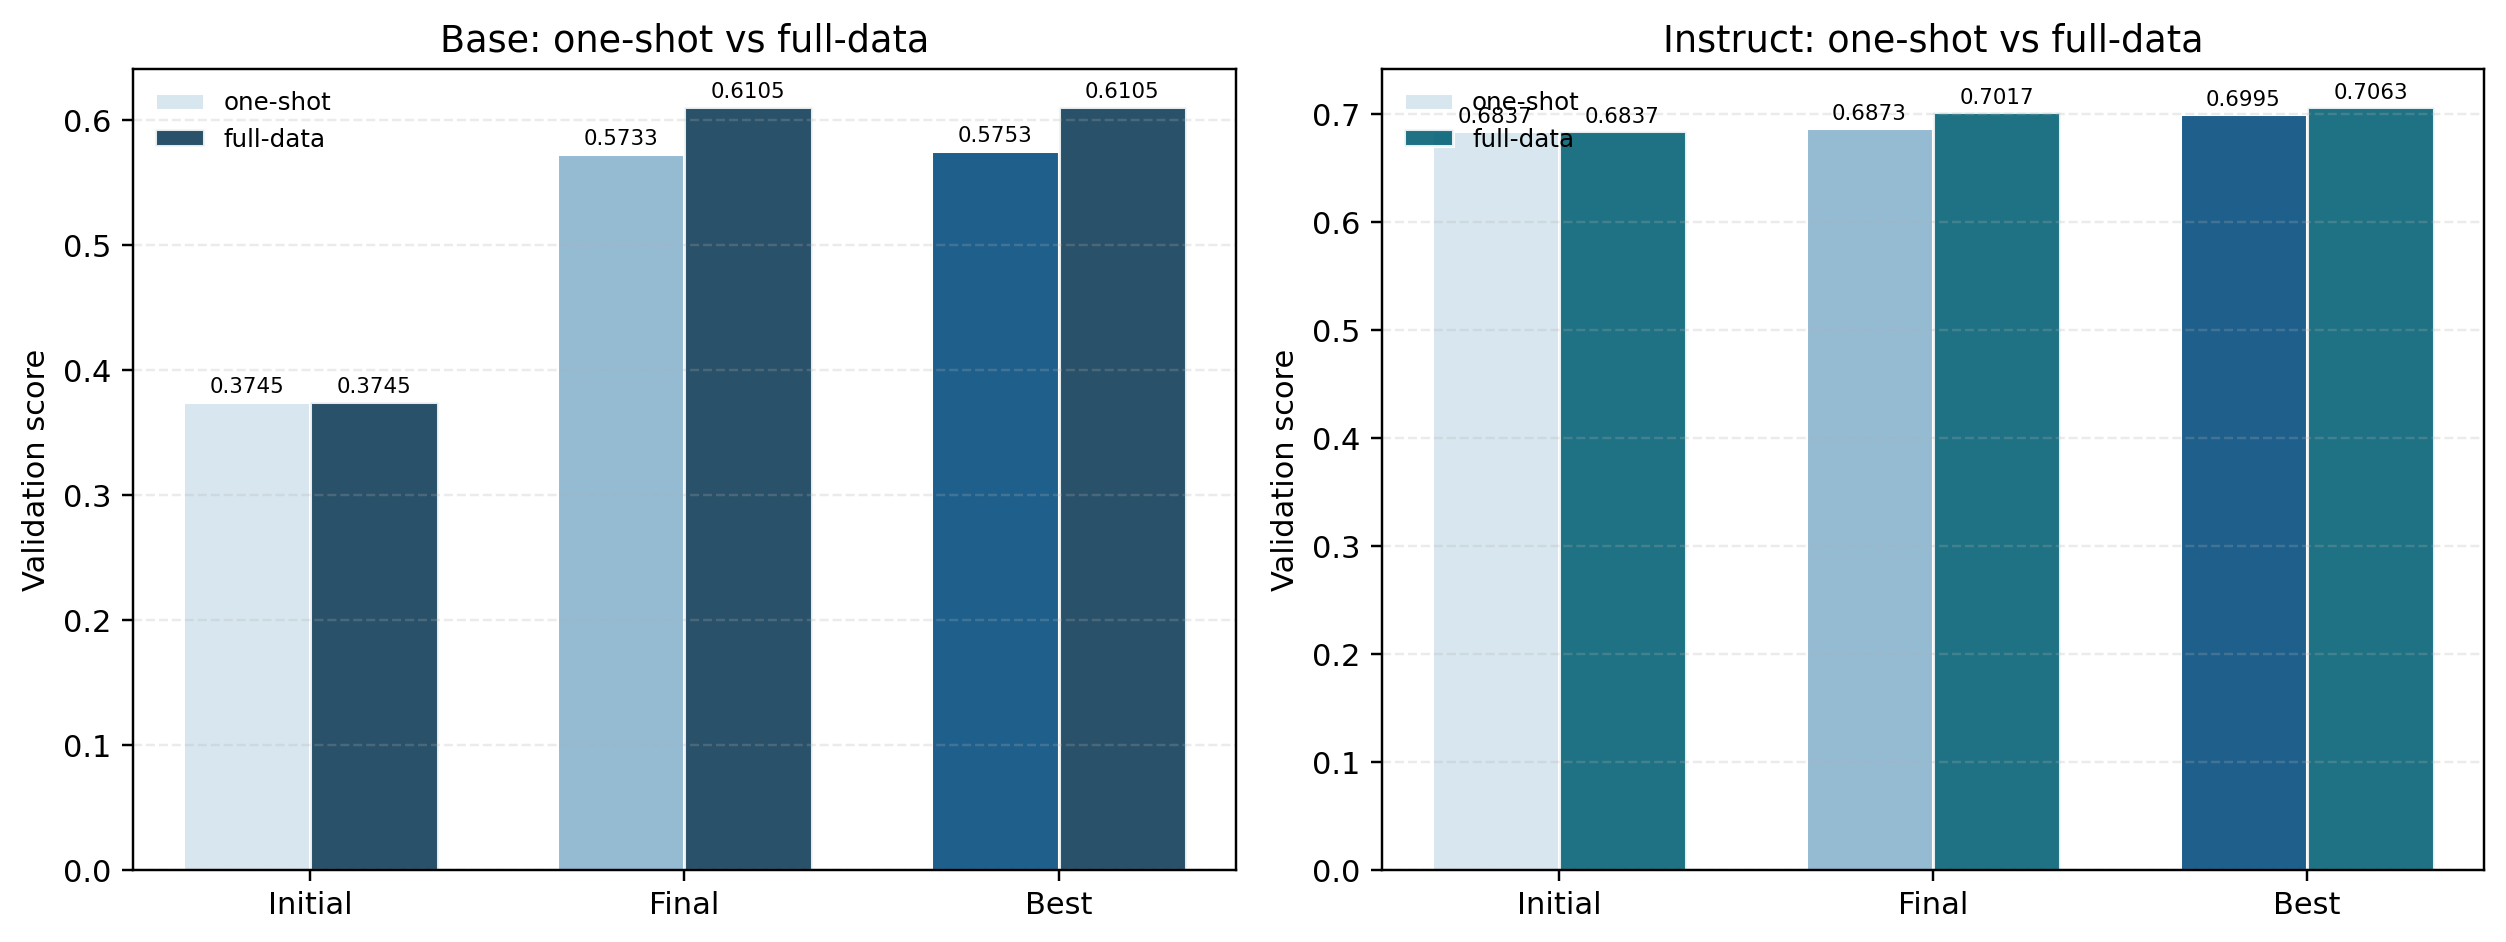
\includegraphics[width=\textwidth]{matched-full-data-panel.png}
    \caption{Initial, final, and best validation scores for the matched one-shot/full-data pairs in the Base and Instruct families. Expanding the data budget improves both families, but the increment is much larger for the Base family.}
    \label{fig:en-full-data-reference-main}
\end{figure}

Table~\ref{tab:en-full-ceiling-reference} and Figure~\ref{fig:en-full-data-reference-main} therefore serve as primary evidence for the data-budget comparison. They directly quantify how much performance remains available when the data budget is expanded under the same validation protocol and training cadence. The answer is clear in both families, but especially large in the Base family.

\section{Main Results}

\subsection{The broad picture}

The overall picture is clear in both tabular and trajectory form: the Base family shows large gains, the Instruct family shows small gains, and the matched full-data runs extend both trajectories upward under the same schedule. Figure~\ref{fig:en-all-score} visualizes this contrast directly.

\begin{figure}[H]
    \centering
    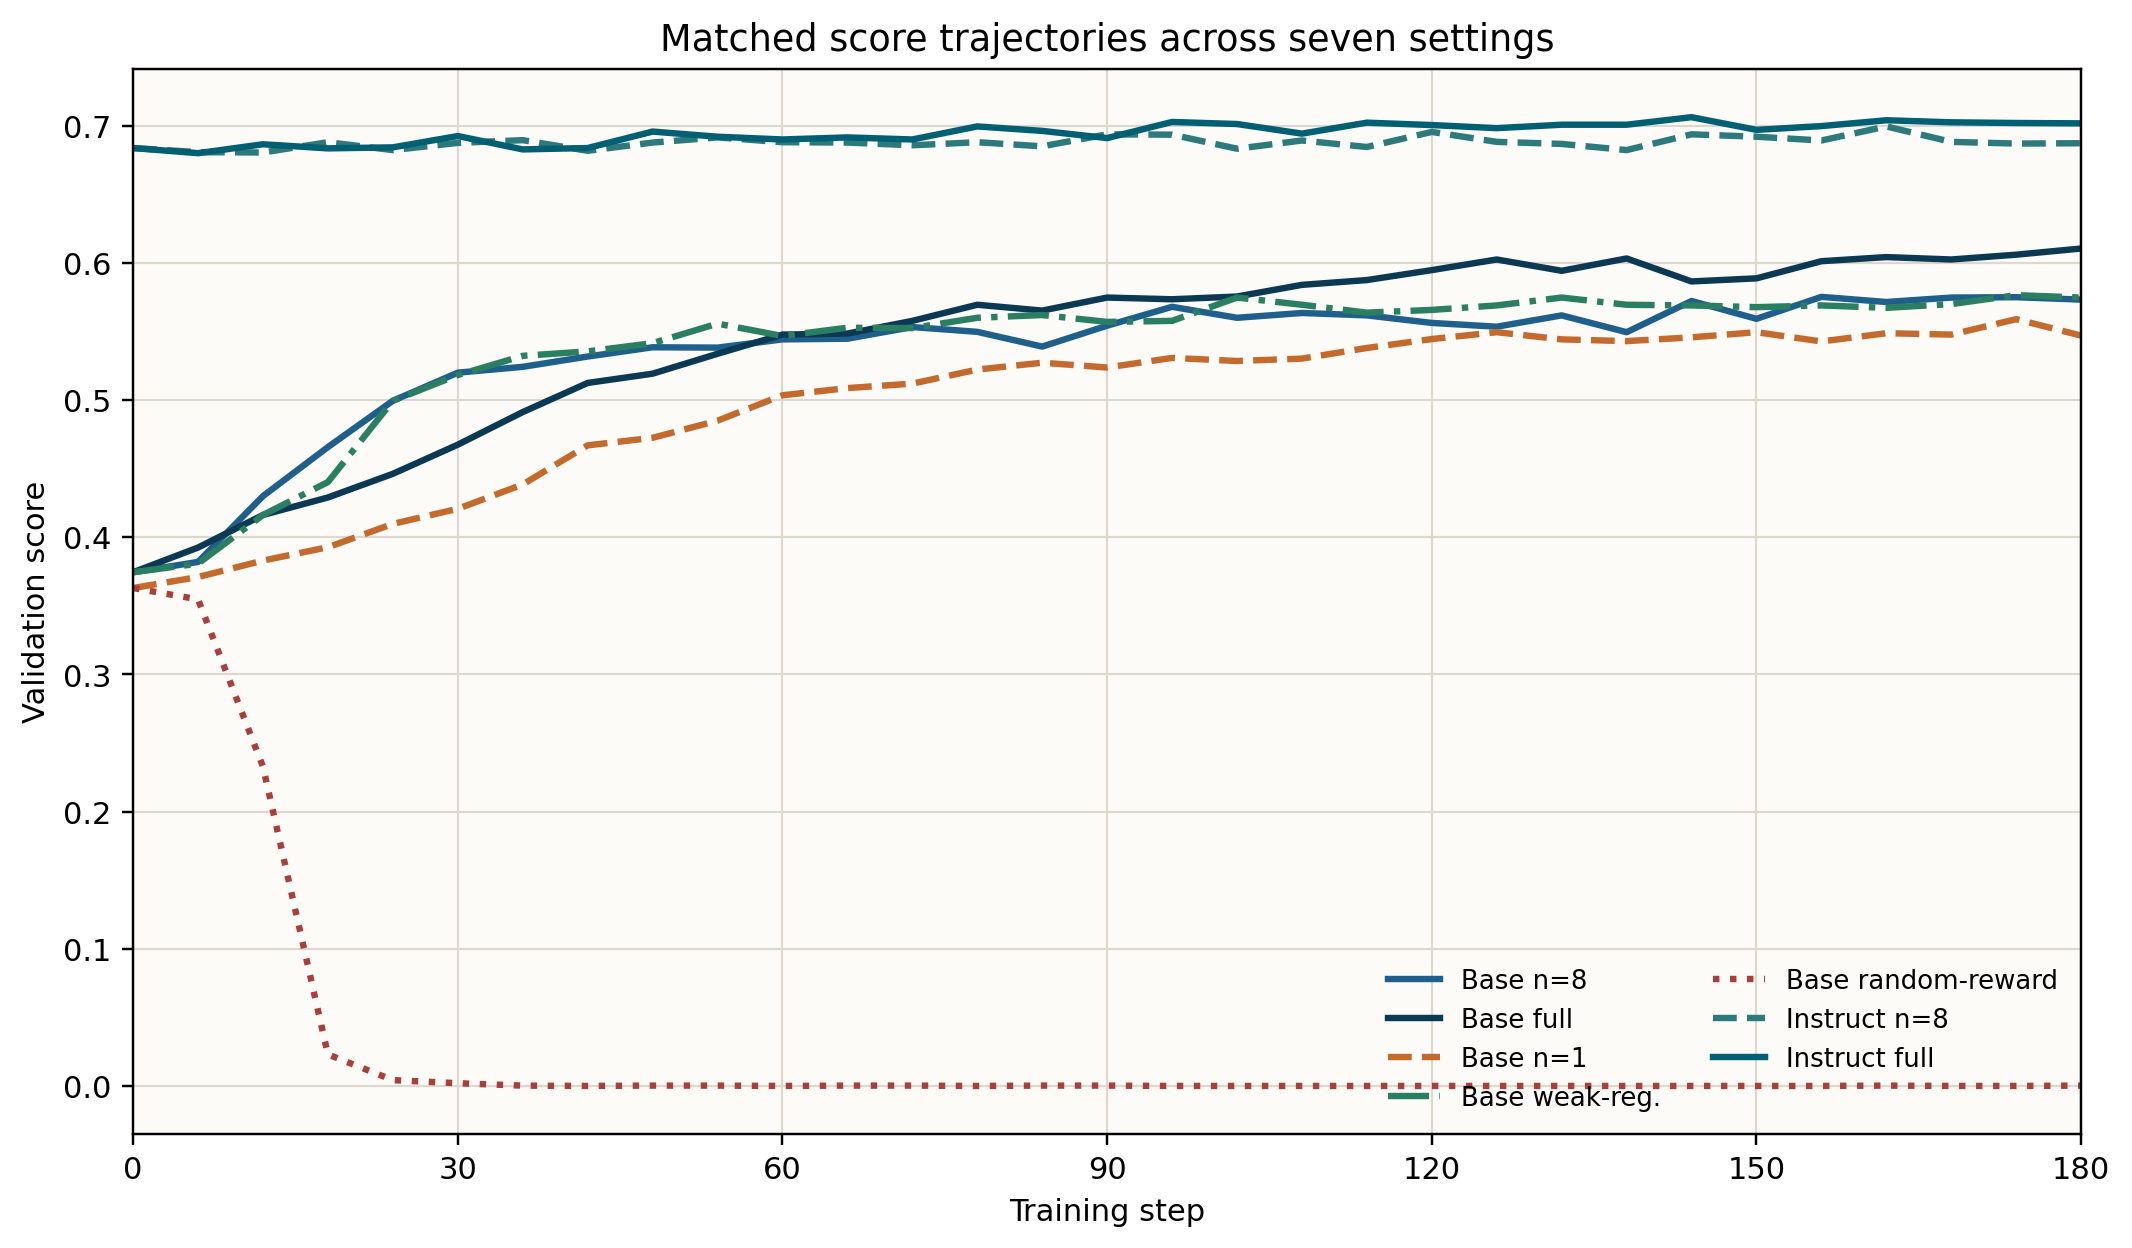
\includegraphics[width=\textwidth]{score-main-seven-settings.png}
    \caption{Validation score trajectories for the seven main settings. The matched full-data curves sit above their one-shot counterparts in both model families, while the Base random-reward condition collapses.}
    \label{fig:en-all-score}
\end{figure}

Figure~\ref{fig:en-all-score} prevents a misleading interpretation of the final table. Final values alone would obscure the fact that the Base curves undergo a genuine phase transition from low to much higher performance, with \texttt{Base full-data} pushing the endpoint still higher, while the Instruct curves mostly oscillate within an already strong range even after the budget expansion to full-data. The scale and shape of improvement are therefore different in kind, not only in magnitude.

\begin{figure}[H]
    \centering
    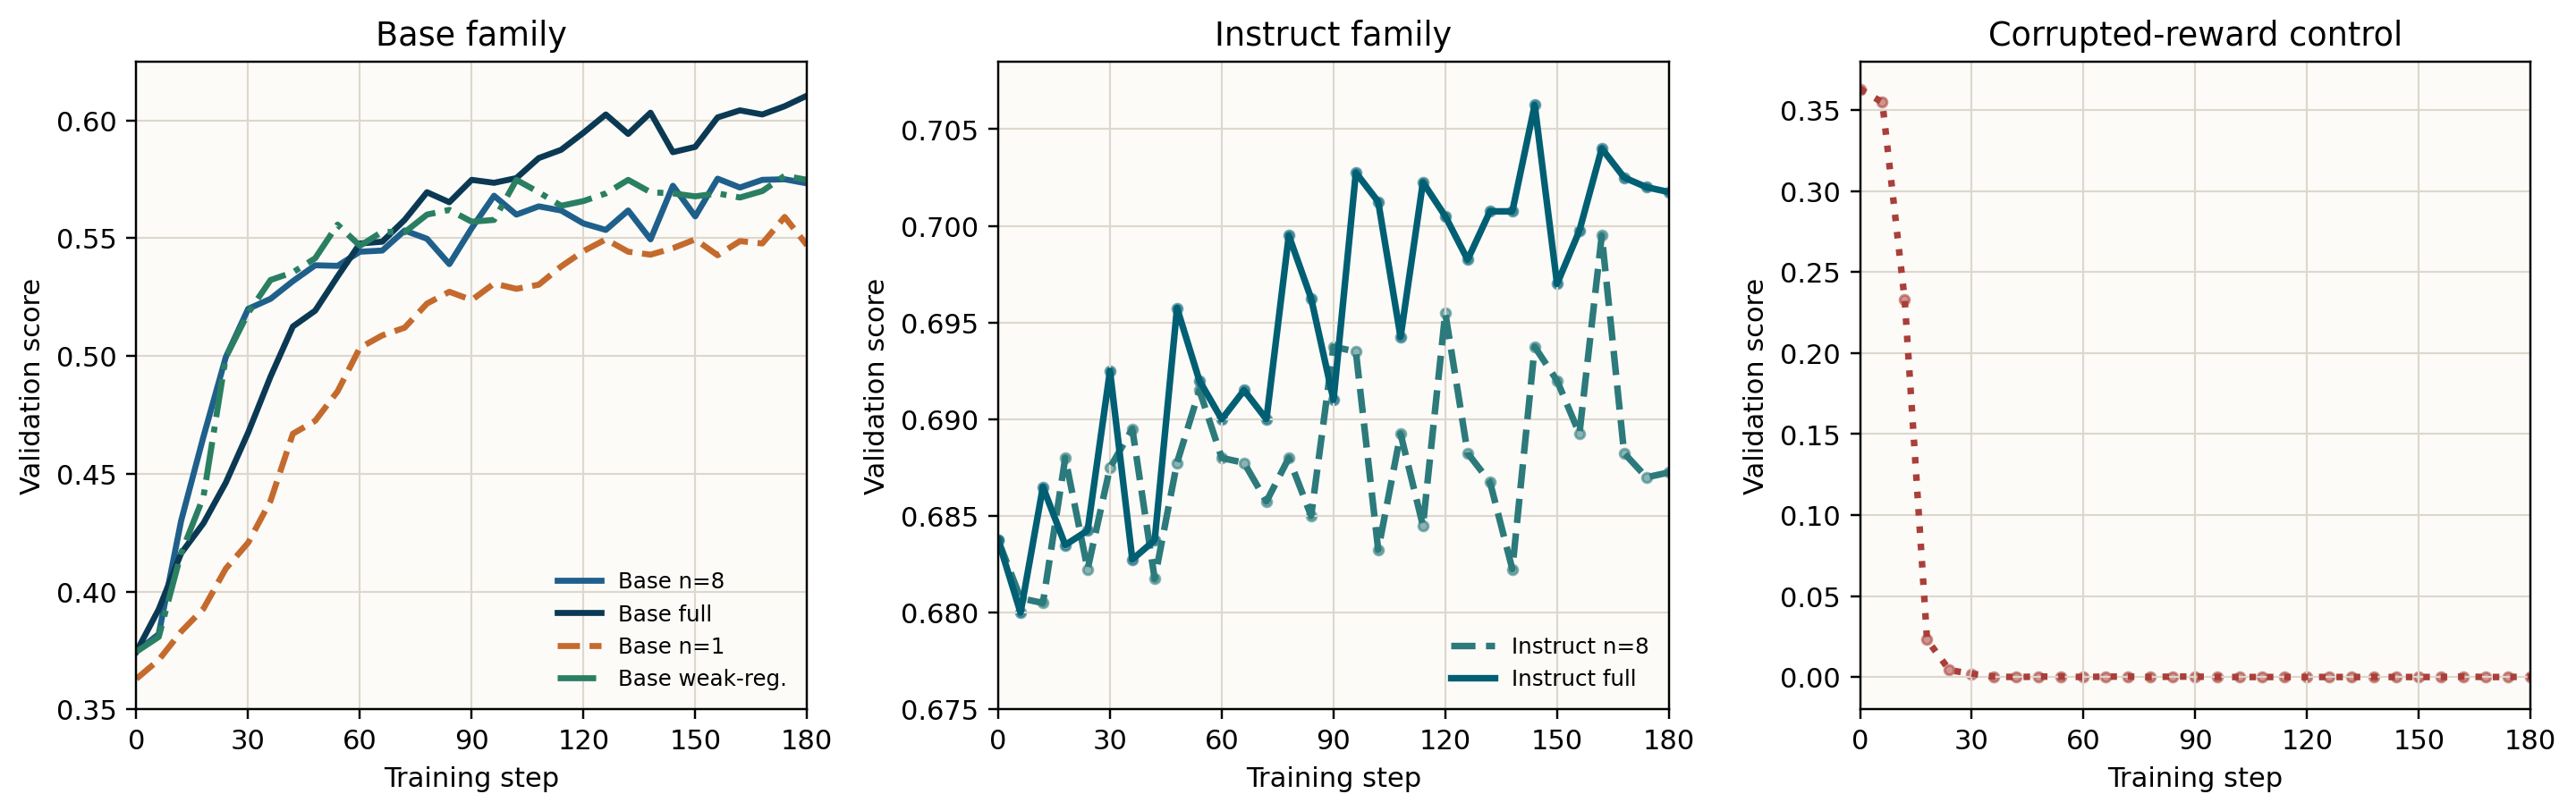
\includegraphics[width=\textwidth]{score-main-detail-panel.png}
    \caption{Zoomed validation-score views for the Base family, the Instruct family, and the random-reward control.}
    \label{fig:en-score-detail-panel}
\end{figure}

Because the seven settings occupy very different score ranges, the global figure is intentionally paired with a zoomed view. Figure~\ref{fig:en-score-detail-panel} resolves two distinctions more clearly. Within the Base family, \texttt{Base full-data} remains visibly above the successful one-shot conditions, while \texttt{Base n=1} stays consistently lower. Within the Instruct family, \texttt{Instruct full-data} is measurably better than \texttt{Instruct n=8}, but the gap remains narrow. The random-reward control can then be read separately as a collapse trajectory rather than as a curve compressed against zero.

\subsection{Base-model gains are large and repeatable}

\texttt{Base n=8} improves from 0.3745 to 0.5733. \texttt{Base weak-reg.} reaches a very similar endpoint at 0.5747, whereas \texttt{Base random-reward} collapses rather than reproducing the meaningful-reward gain. Overall, this pattern shows that the Base-family gains are not an isolated artifact of a single setting. They recur when the reward structure remains meaningful and disappear when the supervision signal is systematically broken.

\begin{figure}[H]
    \centering
    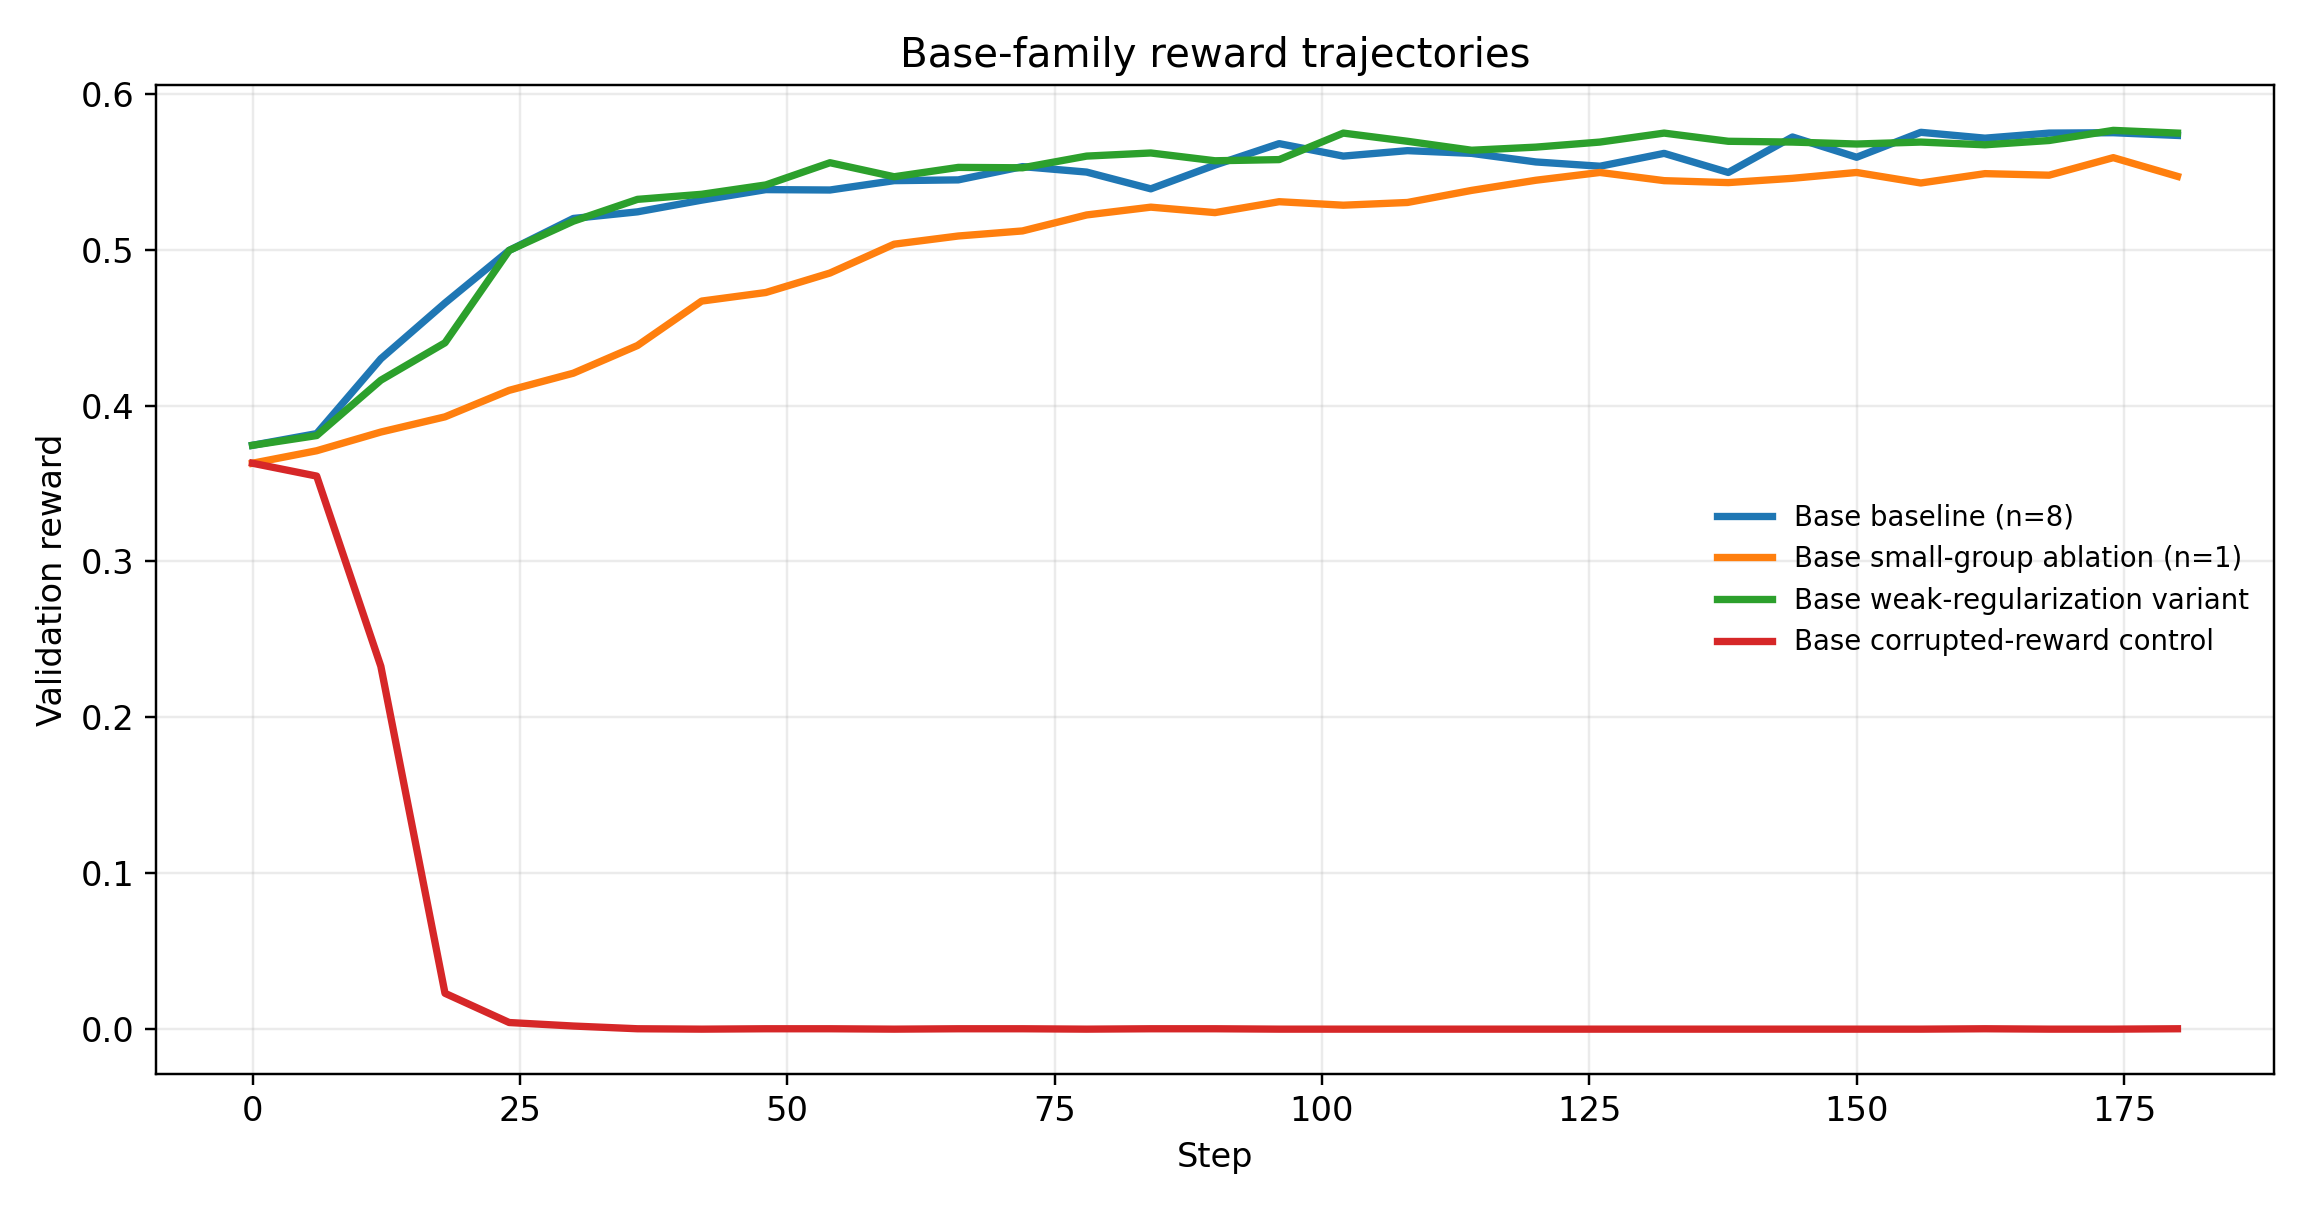
\includegraphics[width=\textwidth]{score-base-static.png}
    \caption{Base-family score trajectories. The family exhibits a pronounced early learning phase followed by higher-level fluctuation.}
    \label{fig:en-base-score}
\end{figure}

\begin{figure}[H]
    \centering
    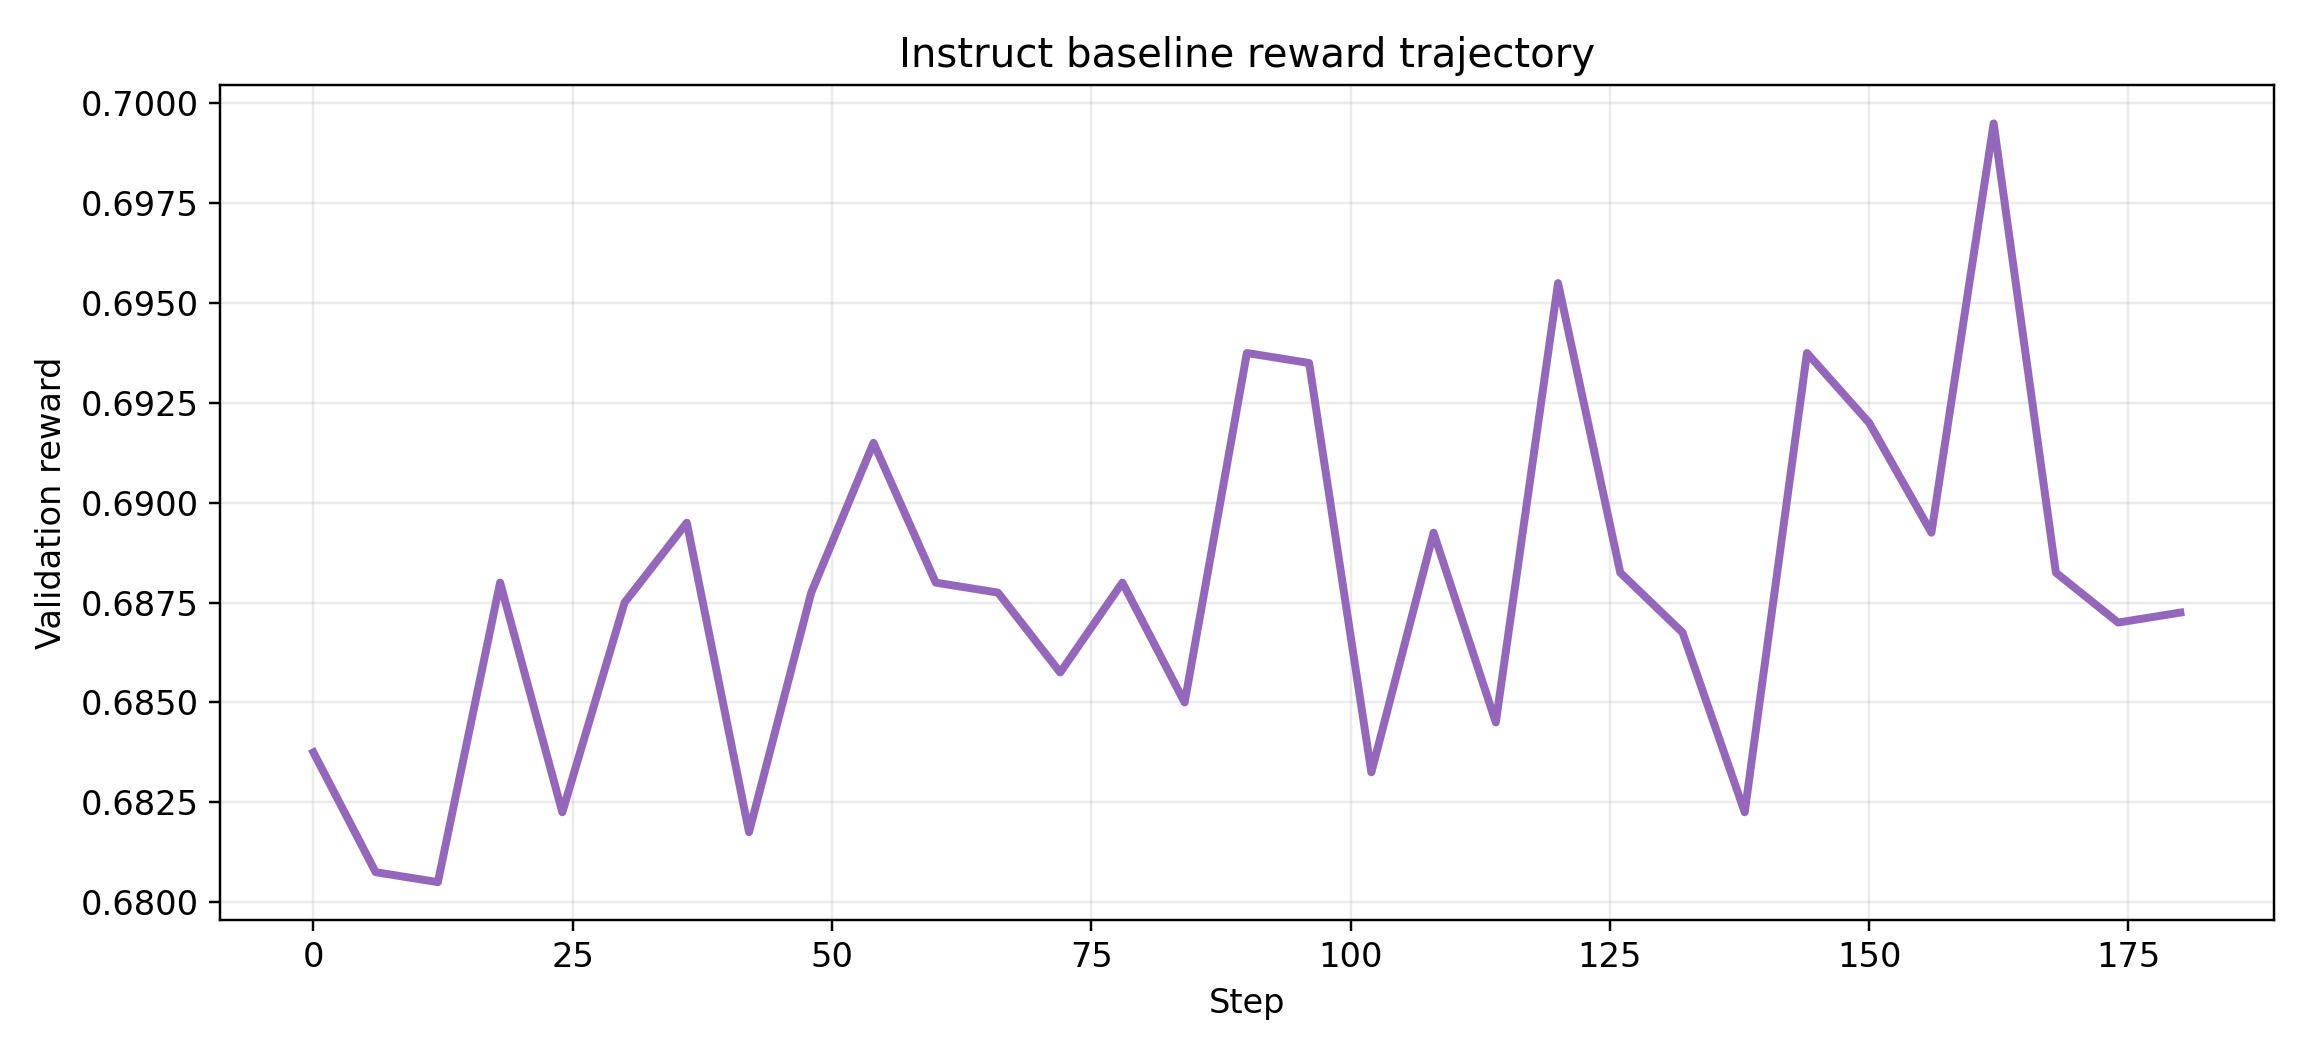
\includegraphics[width=\textwidth]{score-instruct-static.png}
    \caption{Instruct \texttt{n=8} score trajectory. The curve remains in a high but narrow band throughout training.}
    \label{fig:en-instruct-score}
\end{figure}

Figures~\ref{fig:en-base-score} and~\ref{fig:en-instruct-score} also highlight an important training characteristic: the best checkpoint often arrives before the final checkpoint. Low-data RL can enter a late-stage fluctuation regime rather than improving steadily all the way to the end. For future reporting or deployment, selecting the best validated checkpoint is therefore more principled than always taking the last one.

\subsection{The Instruct model starts strong and moves little}

\texttt{Instruct n=8} begins at 0.6837, far above the Base starting point. Its final value is 0.6873, with a best score of 0.6995 at step 162. These are respectable numbers, but the gain scale is tiny compared with the Base family. This pattern is consistent with an Instruct prior that already encodes much of the behavior that low-data GRPO can reasonably refine.

This difference matters for interpretation. A statement of uniform effectiveness across model families would be imprecise. A more accurate statement is that 1-shot GRPO is most useful when there is substantial behavioral slack to correct. The Base model has such slack; the Instruct model has much less.

\section{Behavioral Evidence: Aggregate and Token-Level Views}

\subsection{Base-family behavioral changes}

The Base-family gains are not just visible in score. They co-occur with a coordinated set of behavioral changes. Table~\ref{tab:en-behavior-results} summarizes the final behavioral metrics for all settings, and Figures~\ref{fig:en-base-length} through~\ref{fig:en-base-eos} show how the main Base-family metrics evolve through training.

\begin{table}[H]
    \centering
    \caption{Final behavioral metrics for the seven main-result settings}
    \label{tab:en-behavior-results}
    \begin{threeparttable}
    \small
    \setlength{\tabcolsep}{3.5pt}
    \begin{tabularx}{\textwidth}{>{\raggedright\arraybackslash}p{0.27\textwidth}*{6}{>{\centering\arraybackslash}X}}
        \toprule
        Setting & len. & tail & low-conf & entropy & EOS & top-1 \\
        \midrule
        Base n=8 & 603.1 & 0.9331 & 0.0325 & 0.1839 & 0.9880 & 0.9354 \\
        Base full-data & 536.0 & 0.9320 & 0.0308 & 0.1718 & 0.9549 & 0.9378 \\
        Base n=1 & 580.4 & 0.9003 & 0.0488 & 0.2811 & 0.9215 & 0.9227 \\
        Base weak-reg. & 578.6 & 0.9437 & 0.0294 & 0.1563 & 0.9738 & 0.9437 \\
        Base random-reward & 1192.4 & 0.0001 & 1.0000 & 11.5466 & 0.0009 & 0.0021 \\
        Instruct n=8 & 470.3 & 0.9571 & 0.0187 & 0.1322 & 0.9926 & 0.9634 \\
        Instruct full-data & 452.7 & 0.9673 & 0.0115 & 0.0837 & 0.9983 & 0.9710 \\
        \bottomrule
    \end{tabularx}
    \begin{tablenotes}[flushleft]
        \footnotesize
        \item Note: Short labels follow the seven main-result settings. ``len.'' denotes response length; ``tail'', ``EOS'', and ``top-1'' denote tail confidence, final EOS probability, and mean top-1 probability.
    \end{tablenotes}
\end{threeparttable}
\end{table}

The seven-setting behavioral view makes the matched full-data runs part of the mechanism evidence rather than only score-level references. Figure~\ref{fig:en-behavior-detail-main-settings} places the key endpoint-sensitive token metrics in one frame. \texttt{Base full-data} reaches the strongest Base-family final score while also shortening responses, lowering low-confidence mass, lowering token entropy, and increasing top-1 probability relative to \texttt{Base n=8}. \texttt{Instruct full-data} shows the same direction of movement relative to \texttt{Instruct n=8}, but from a much stronger starting region and with a smaller score gain. Thus, expanding the data budget does not create a qualitatively different behavior profile; it extends the same stabilization pattern.

\begin{figure}[H]
    \centering
    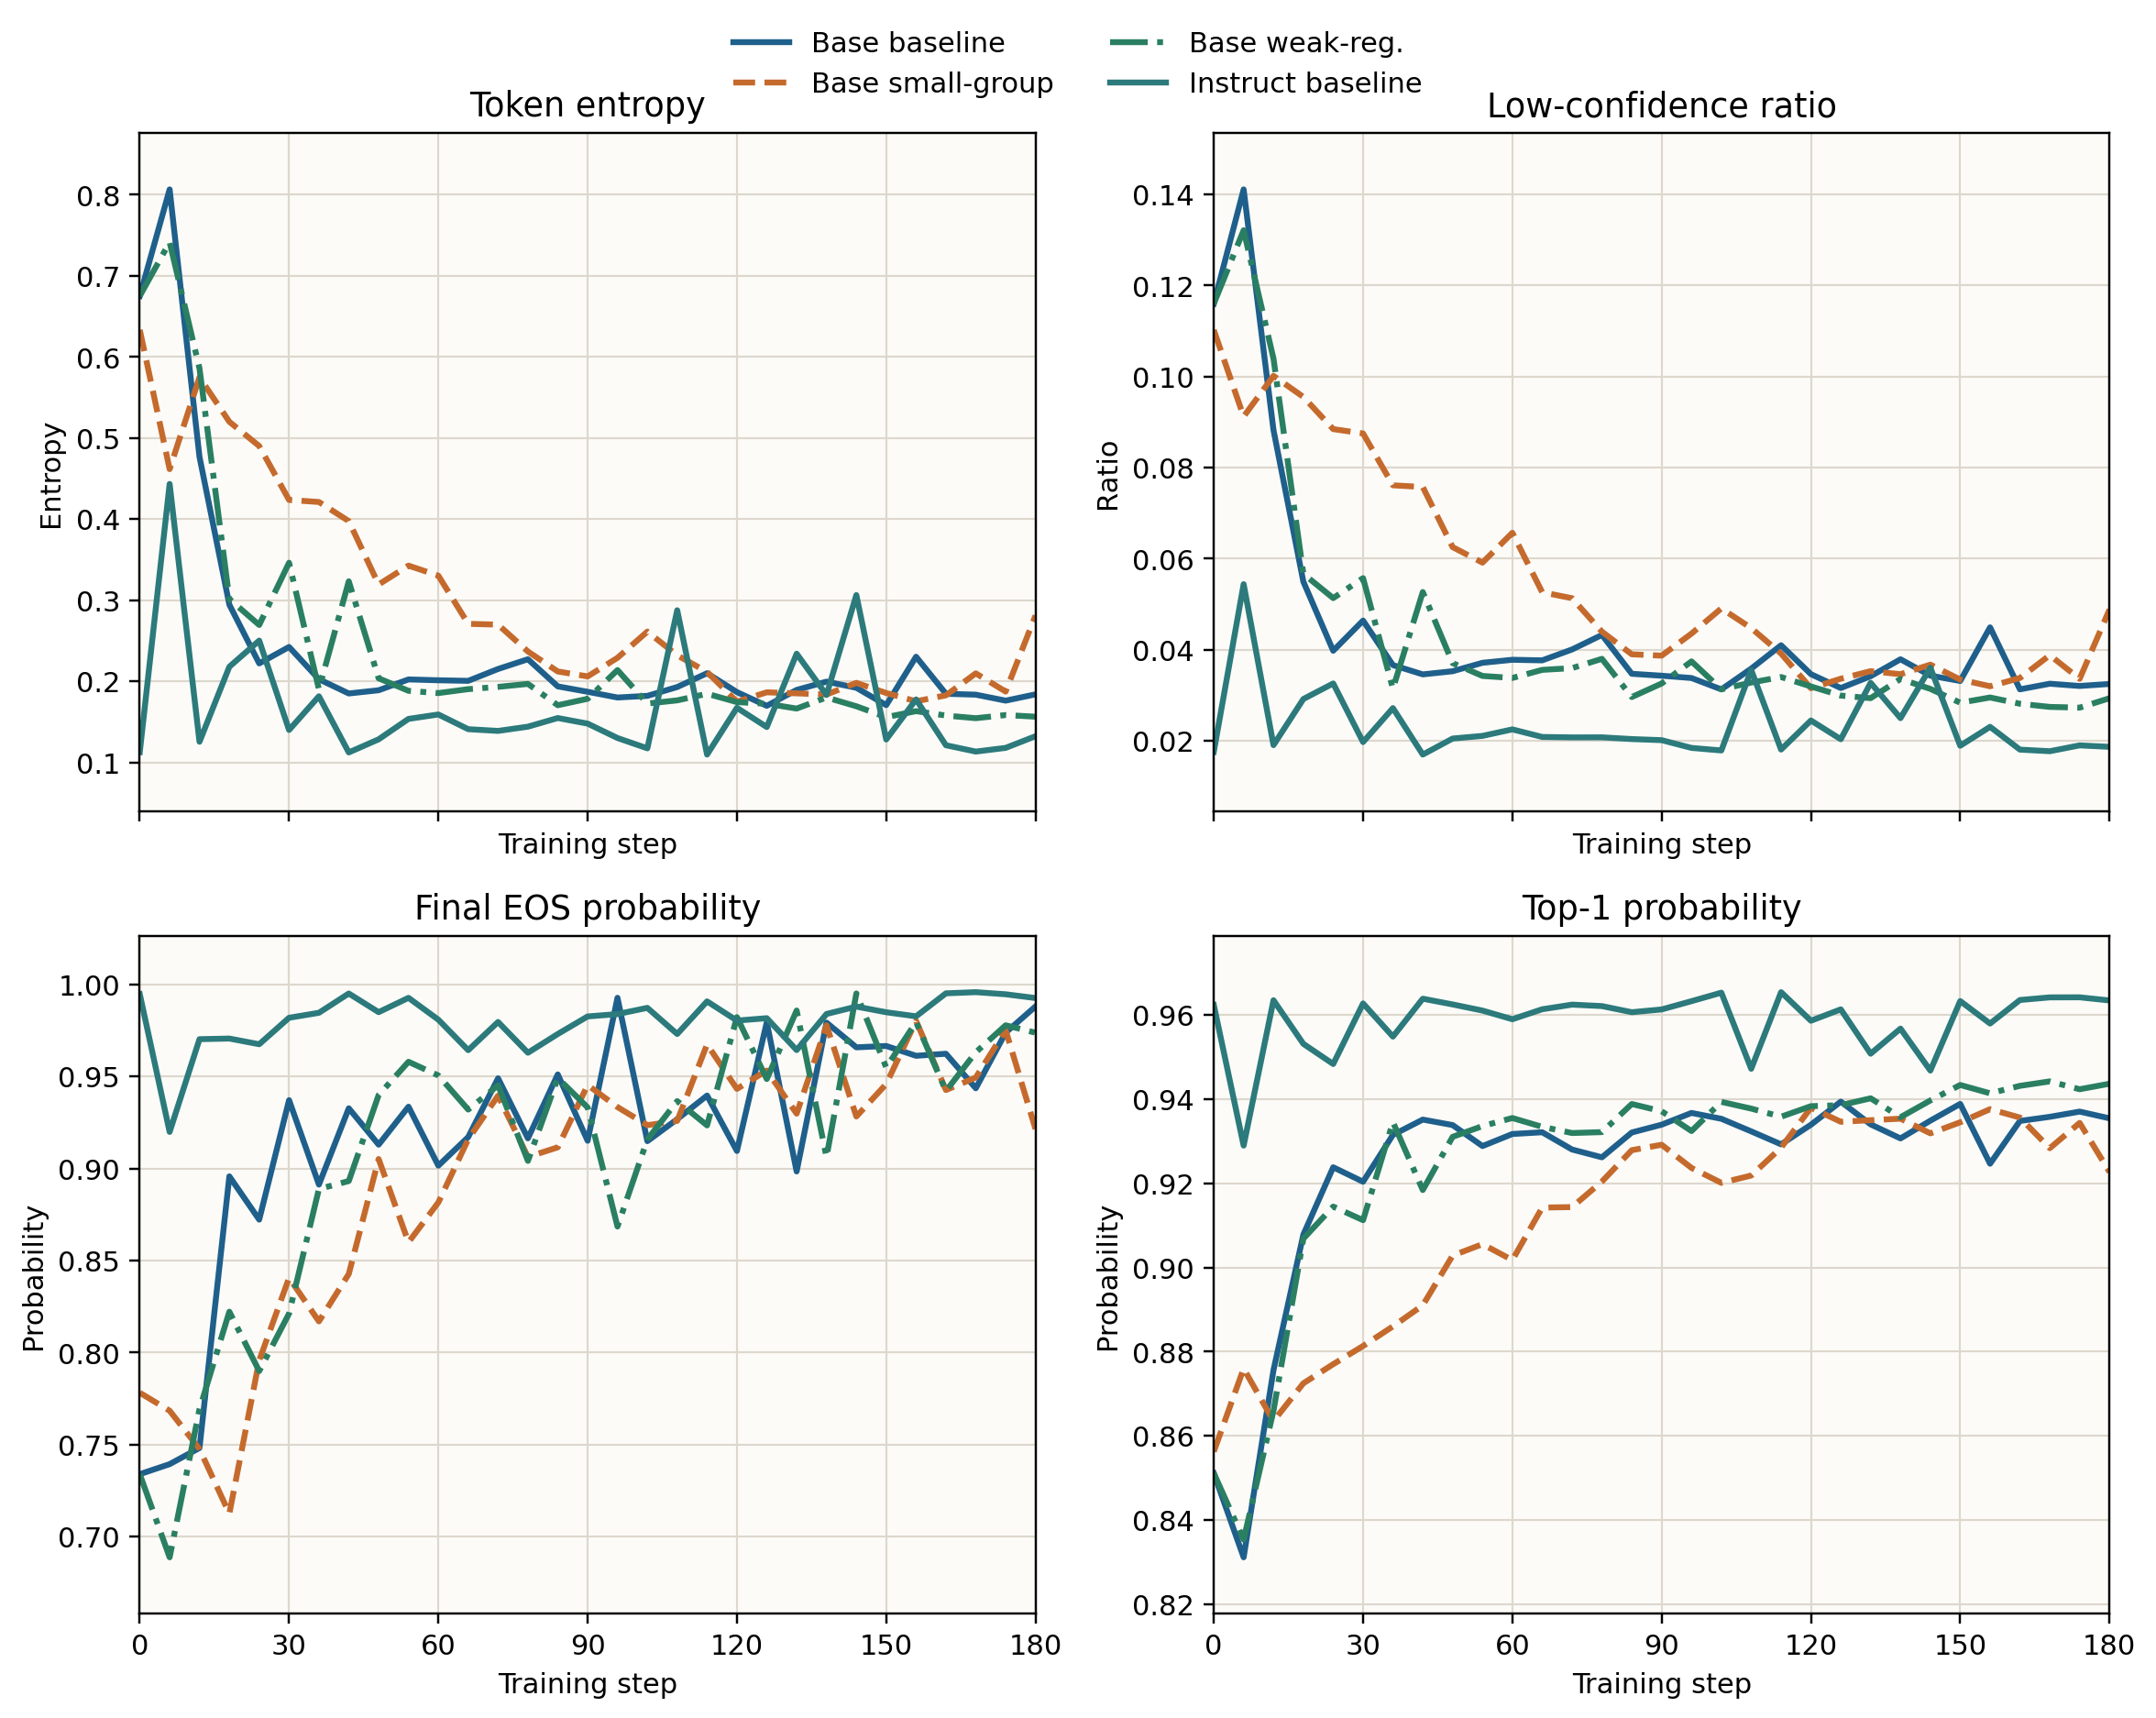
\includegraphics[width=\textwidth]{behavior-detail-main-settings-panel.png}
    \caption{Aggregate token-behavior comparison across the seven main-result settings.}
    \label{fig:en-behavior-detail-main-settings}
\end{figure}

This view also clarifies why the random-reward control is analytically useful. It is not merely a weak version of the successful settings. Its entropy rises to 11.5466, its low-confidence ratio reaches 1.0000, and its mean top-1 probability falls to 0.0021. In other words, corrupted reward pushes the model into a qualitatively unstable token-distribution regime, whereas both one-shot and full-data meaningful-reward settings move toward shorter and more concentrated outputs.

\begin{figure}[H]
    \centering
    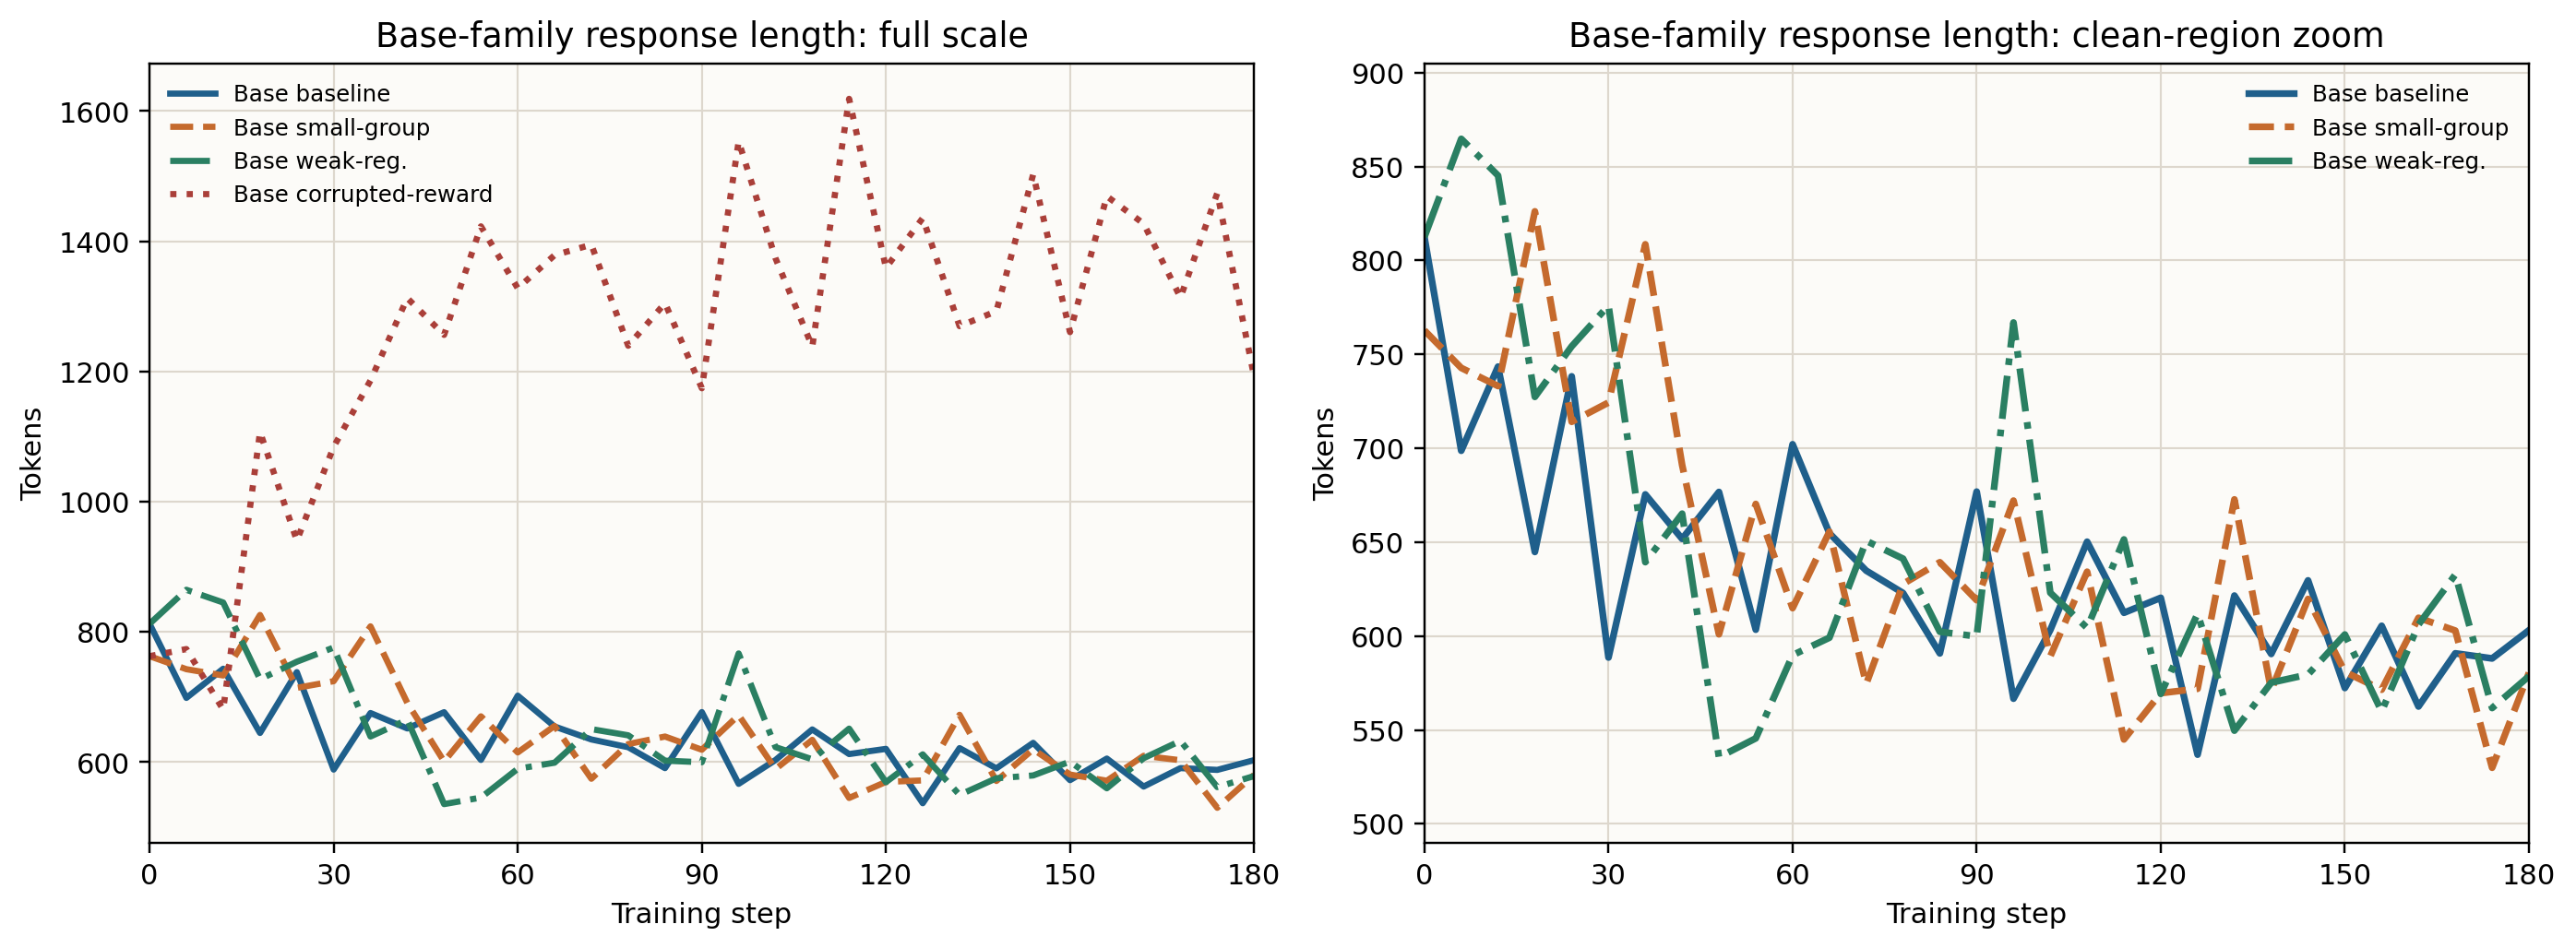
\includegraphics[width=\textwidth]{base-length-static.png}
    \caption{Validation response-length trajectories for the Base-family settings, shown with full-scale and zoomed views.}
    \label{fig:en-base-length}
\end{figure}

\begin{figure}[H]
    \centering
    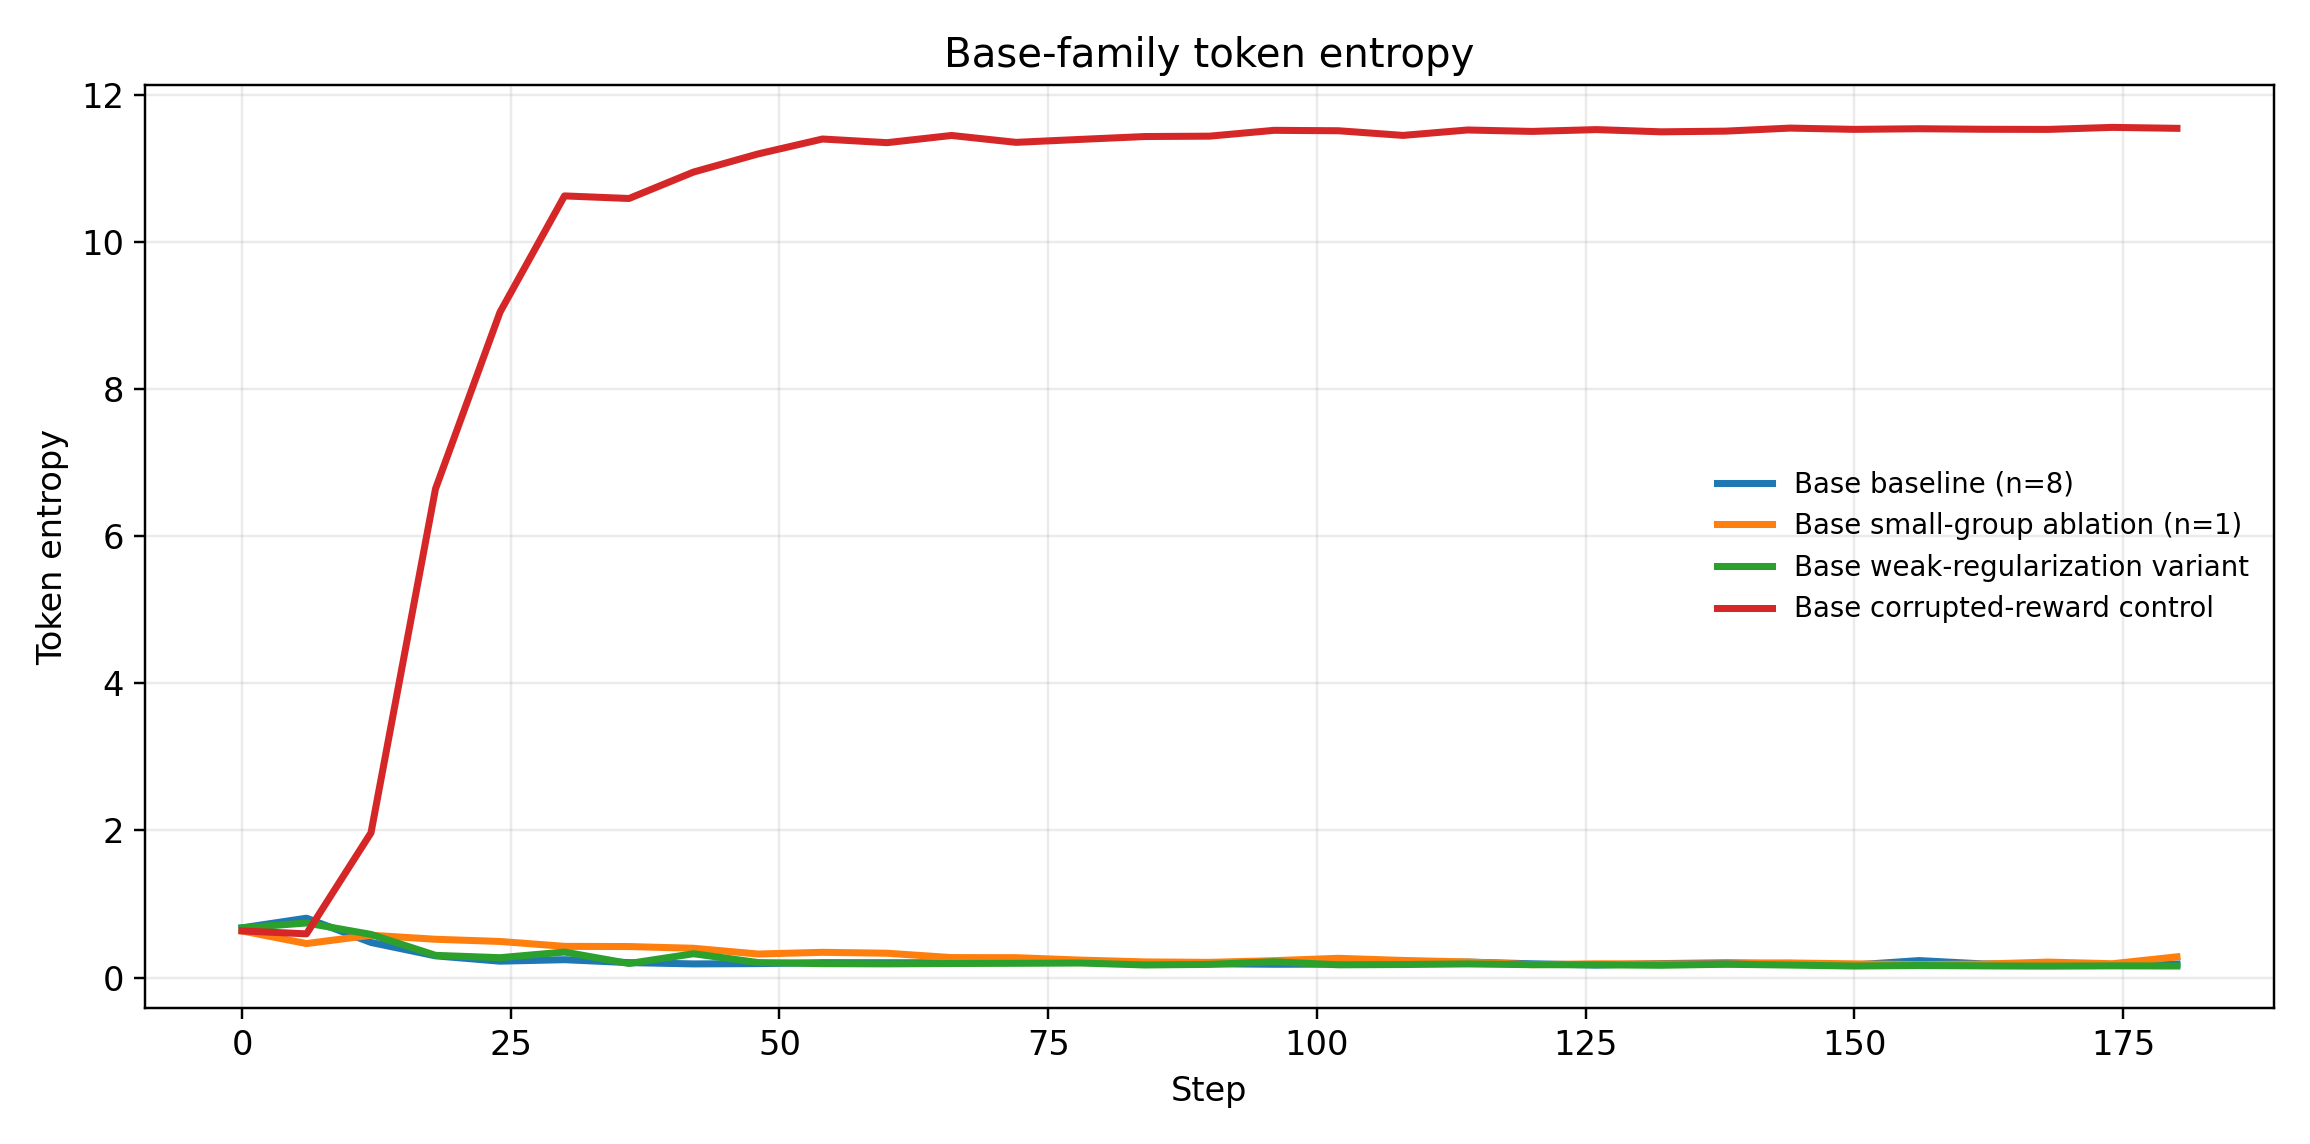
\includegraphics[width=\textwidth]{base-entropy-static.png}
    \caption{Validation token-entropy trajectories for the Base-family settings, shown with full-scale and zoomed views.}
    \label{fig:en-base-entropy}
\end{figure}

\begin{figure}[H]
    \centering
    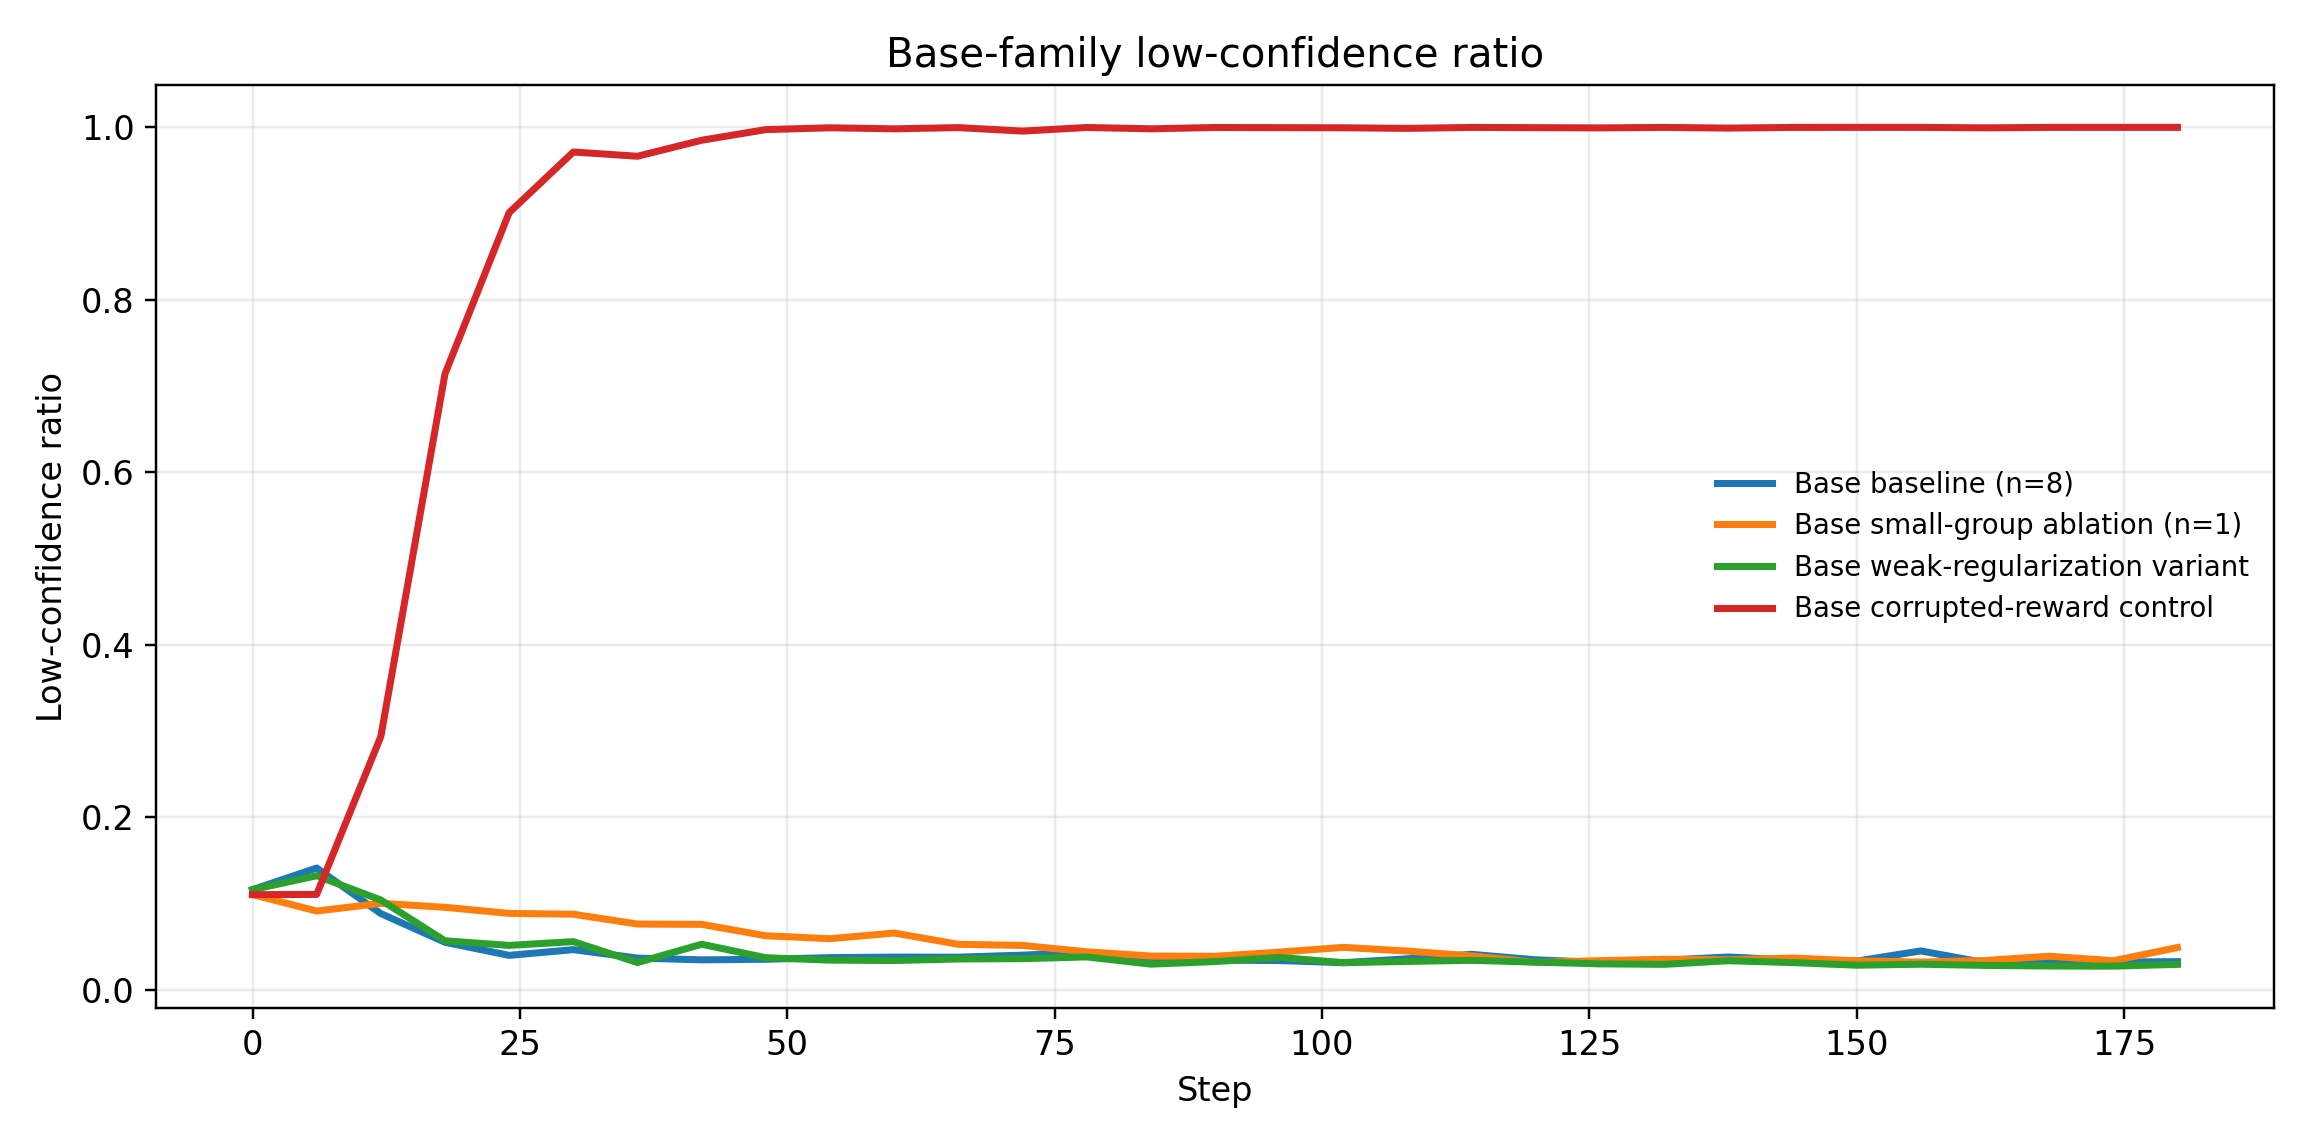
\includegraphics[width=\textwidth]{base-lowconf-static.png}
    \caption{Low-confidence-token trajectories for the Base-family settings, shown with full-scale and zoomed views.}
    \label{fig:en-base-lowconf}
\end{figure}

\begin{figure}[H]
    \centering
    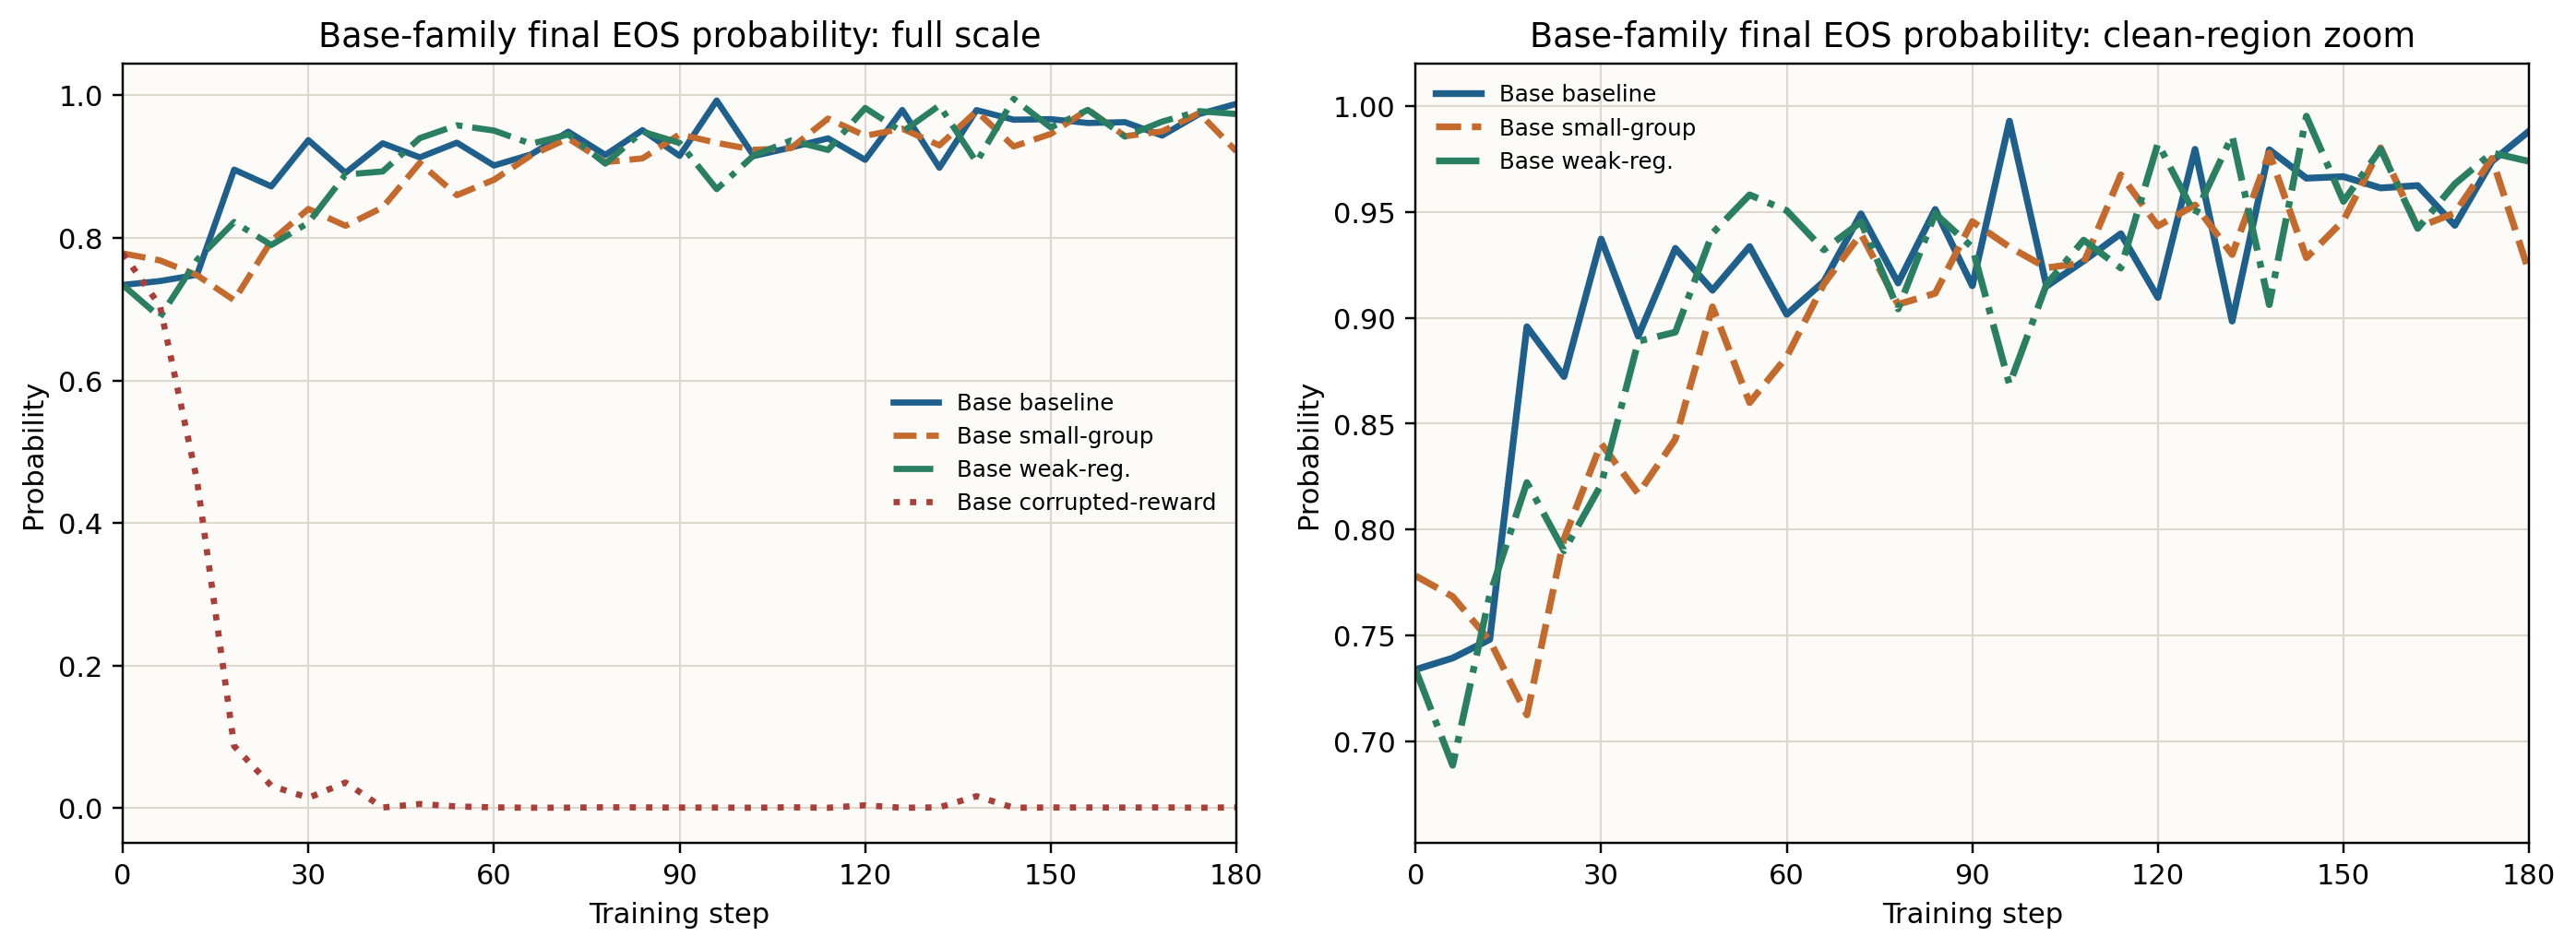
\includegraphics[width=\textwidth]{base-eos-static.png}
    \caption{Final-EOS-probability trajectories for the Base-family settings, shown with full-scale and zoomed views.}
    \label{fig:en-base-eos}
\end{figure}

\begin{figure}[H]
    \centering
    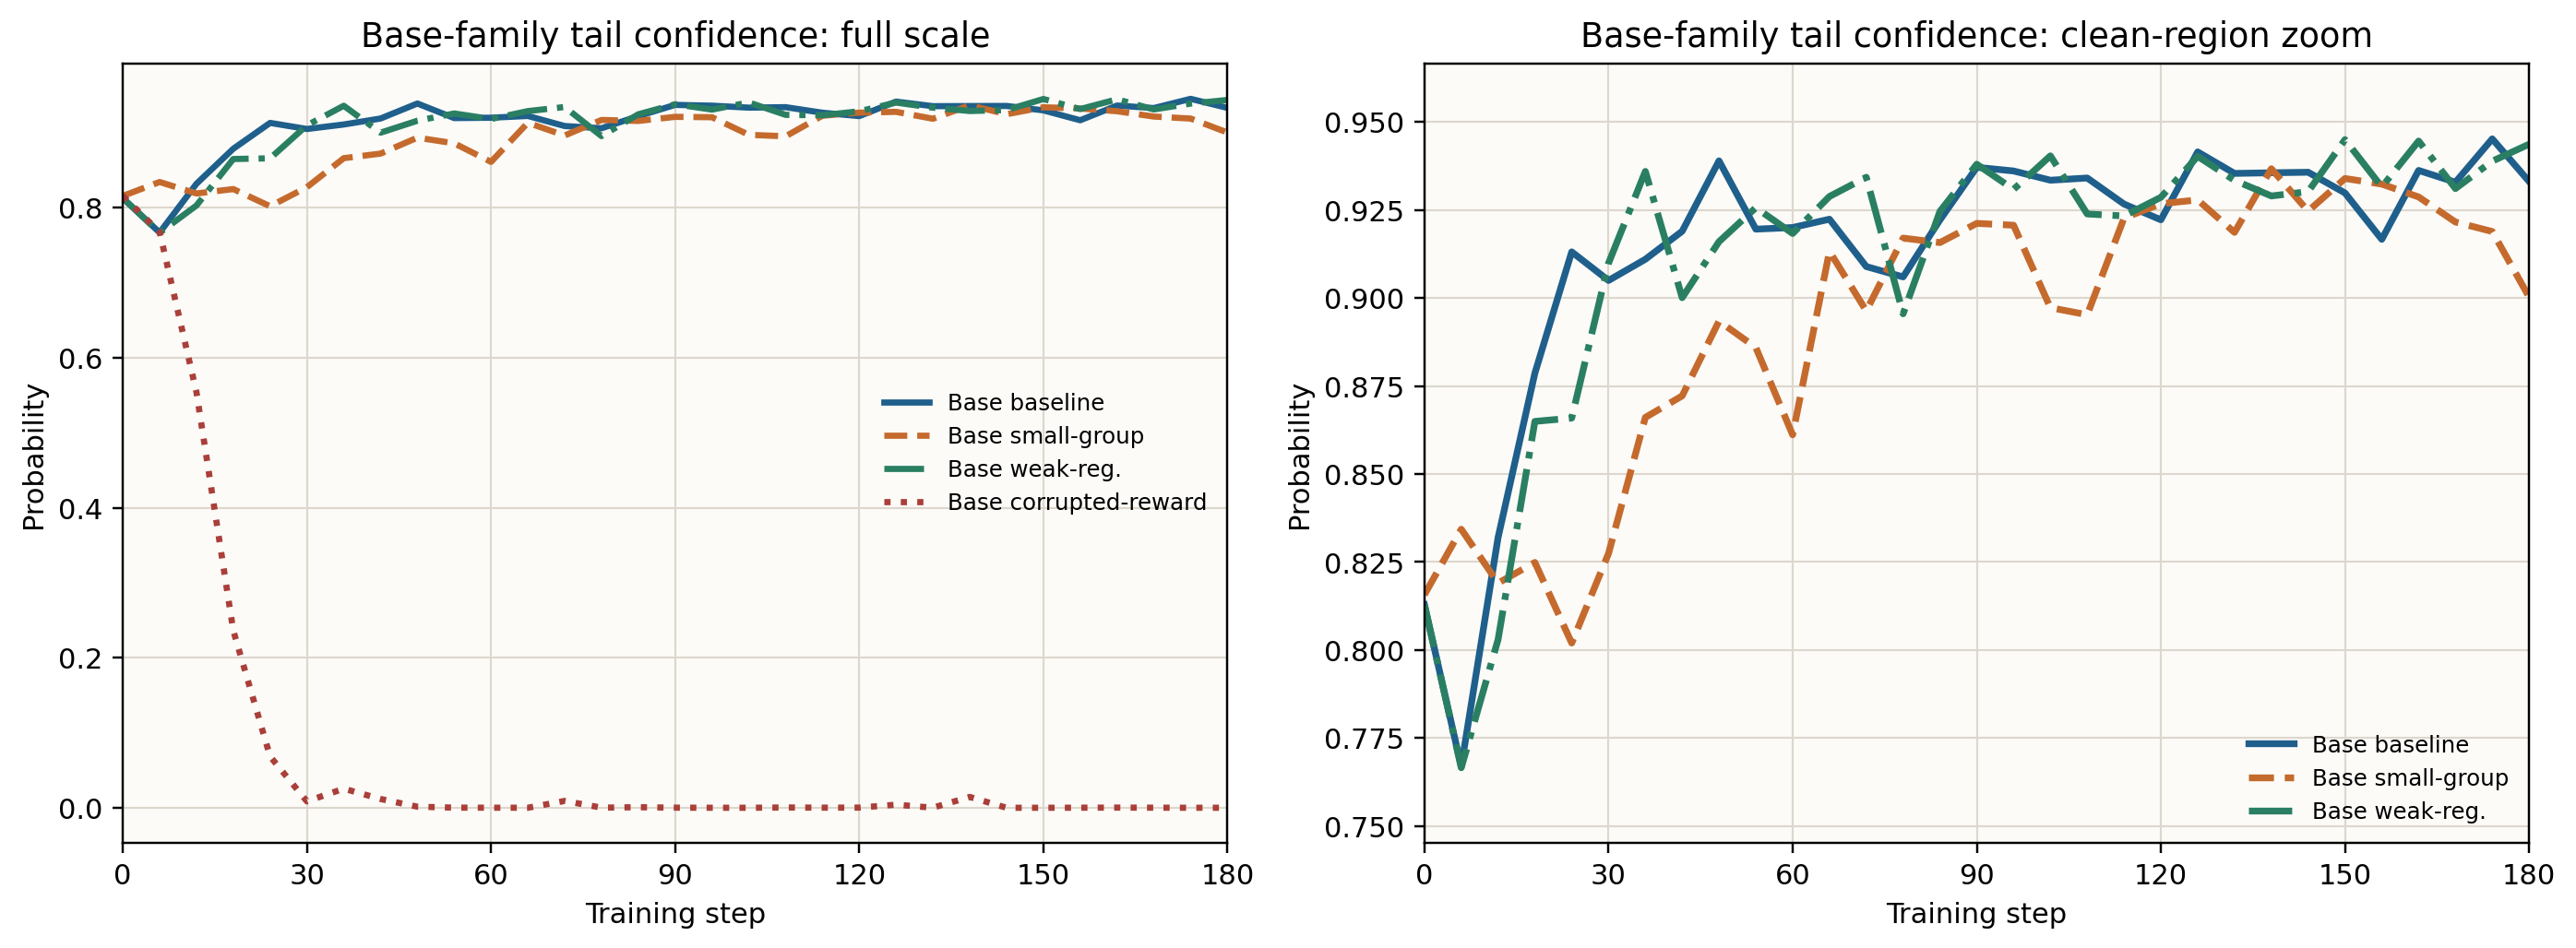
\includegraphics[width=\textwidth]{base-tailconf-static.png}
    \caption{Tail-confidence trajectories for the Base-family settings, shown with full-scale and zoomed views.}
    \label{fig:en-base-tailconf}
\end{figure}

\begin{figure}[H]
    \centering
    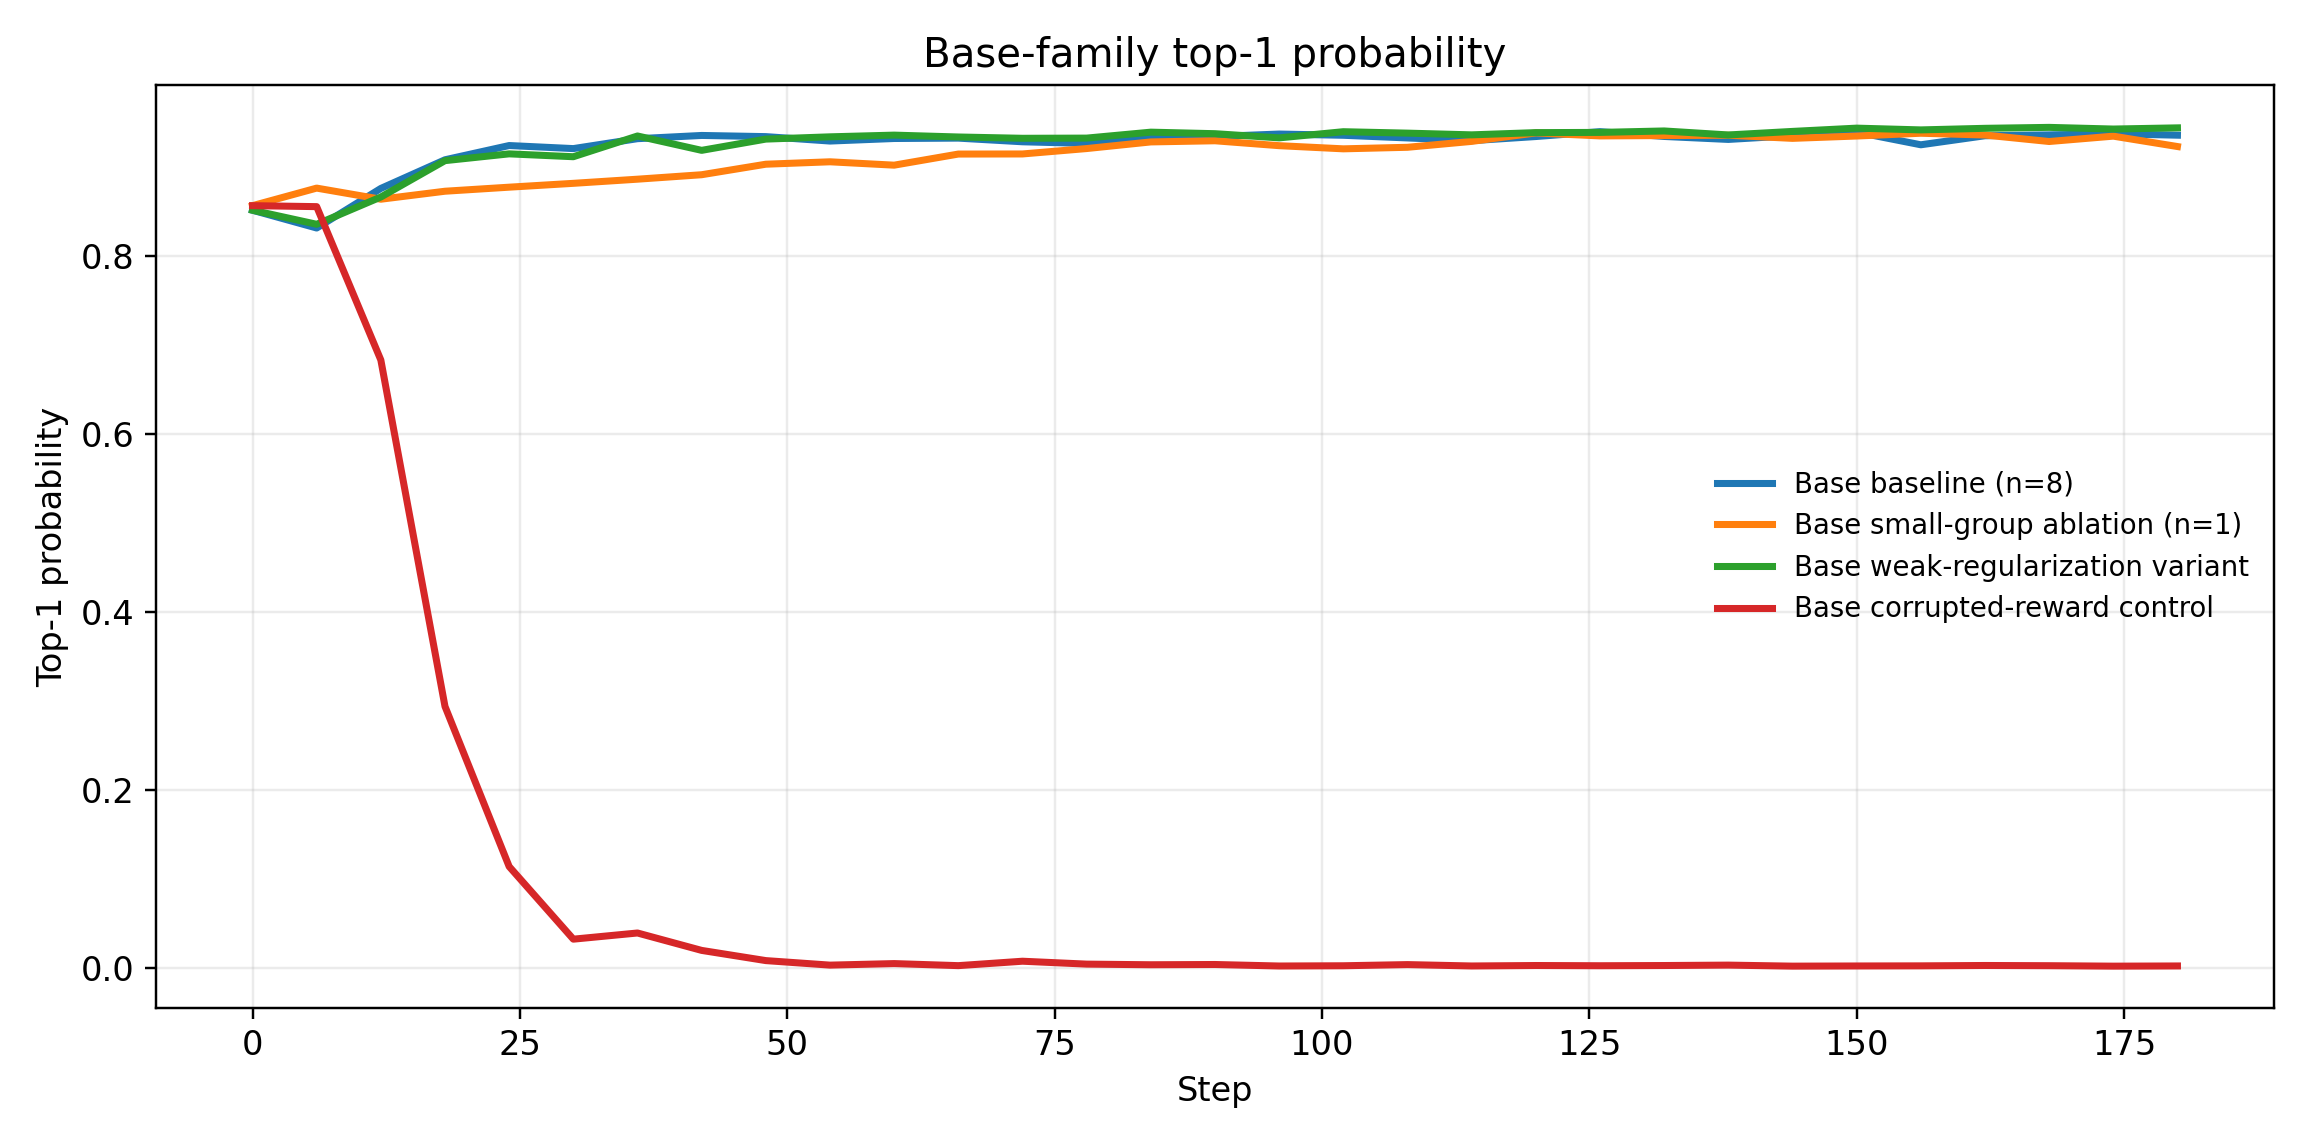
\includegraphics[width=\textwidth]{base-top1-static.png}
    \caption{Mean top-1-probability trajectories for the Base-family settings, shown with full-scale and zoomed views.}
    \label{fig:en-base-top1}
\end{figure}

Figures~\ref{fig:en-base-length} through~\ref{fig:en-base-top1} show a consistent pattern. Each figure uses a full-scale panel plus a meaningful-reward zoom: the full-scale view preserves the abnormal direction of the random-reward setting, whereas the zoomed view prevents that outlier from compressing the differences among successful settings. Outputs get shorter, entropy falls, low-confidence tokens become rarer, and EOS probability increases, while tail confidence and top-1 probability rise. These changes are consistent with the model becoming more decisive and better calibrated. They do not indicate that performance improves through longer or more diffuse chains. Instead, the gains appear to come from a more economical and stable use of the model's existing reasoning ability.

\begin{figure}[H]
    \centering
    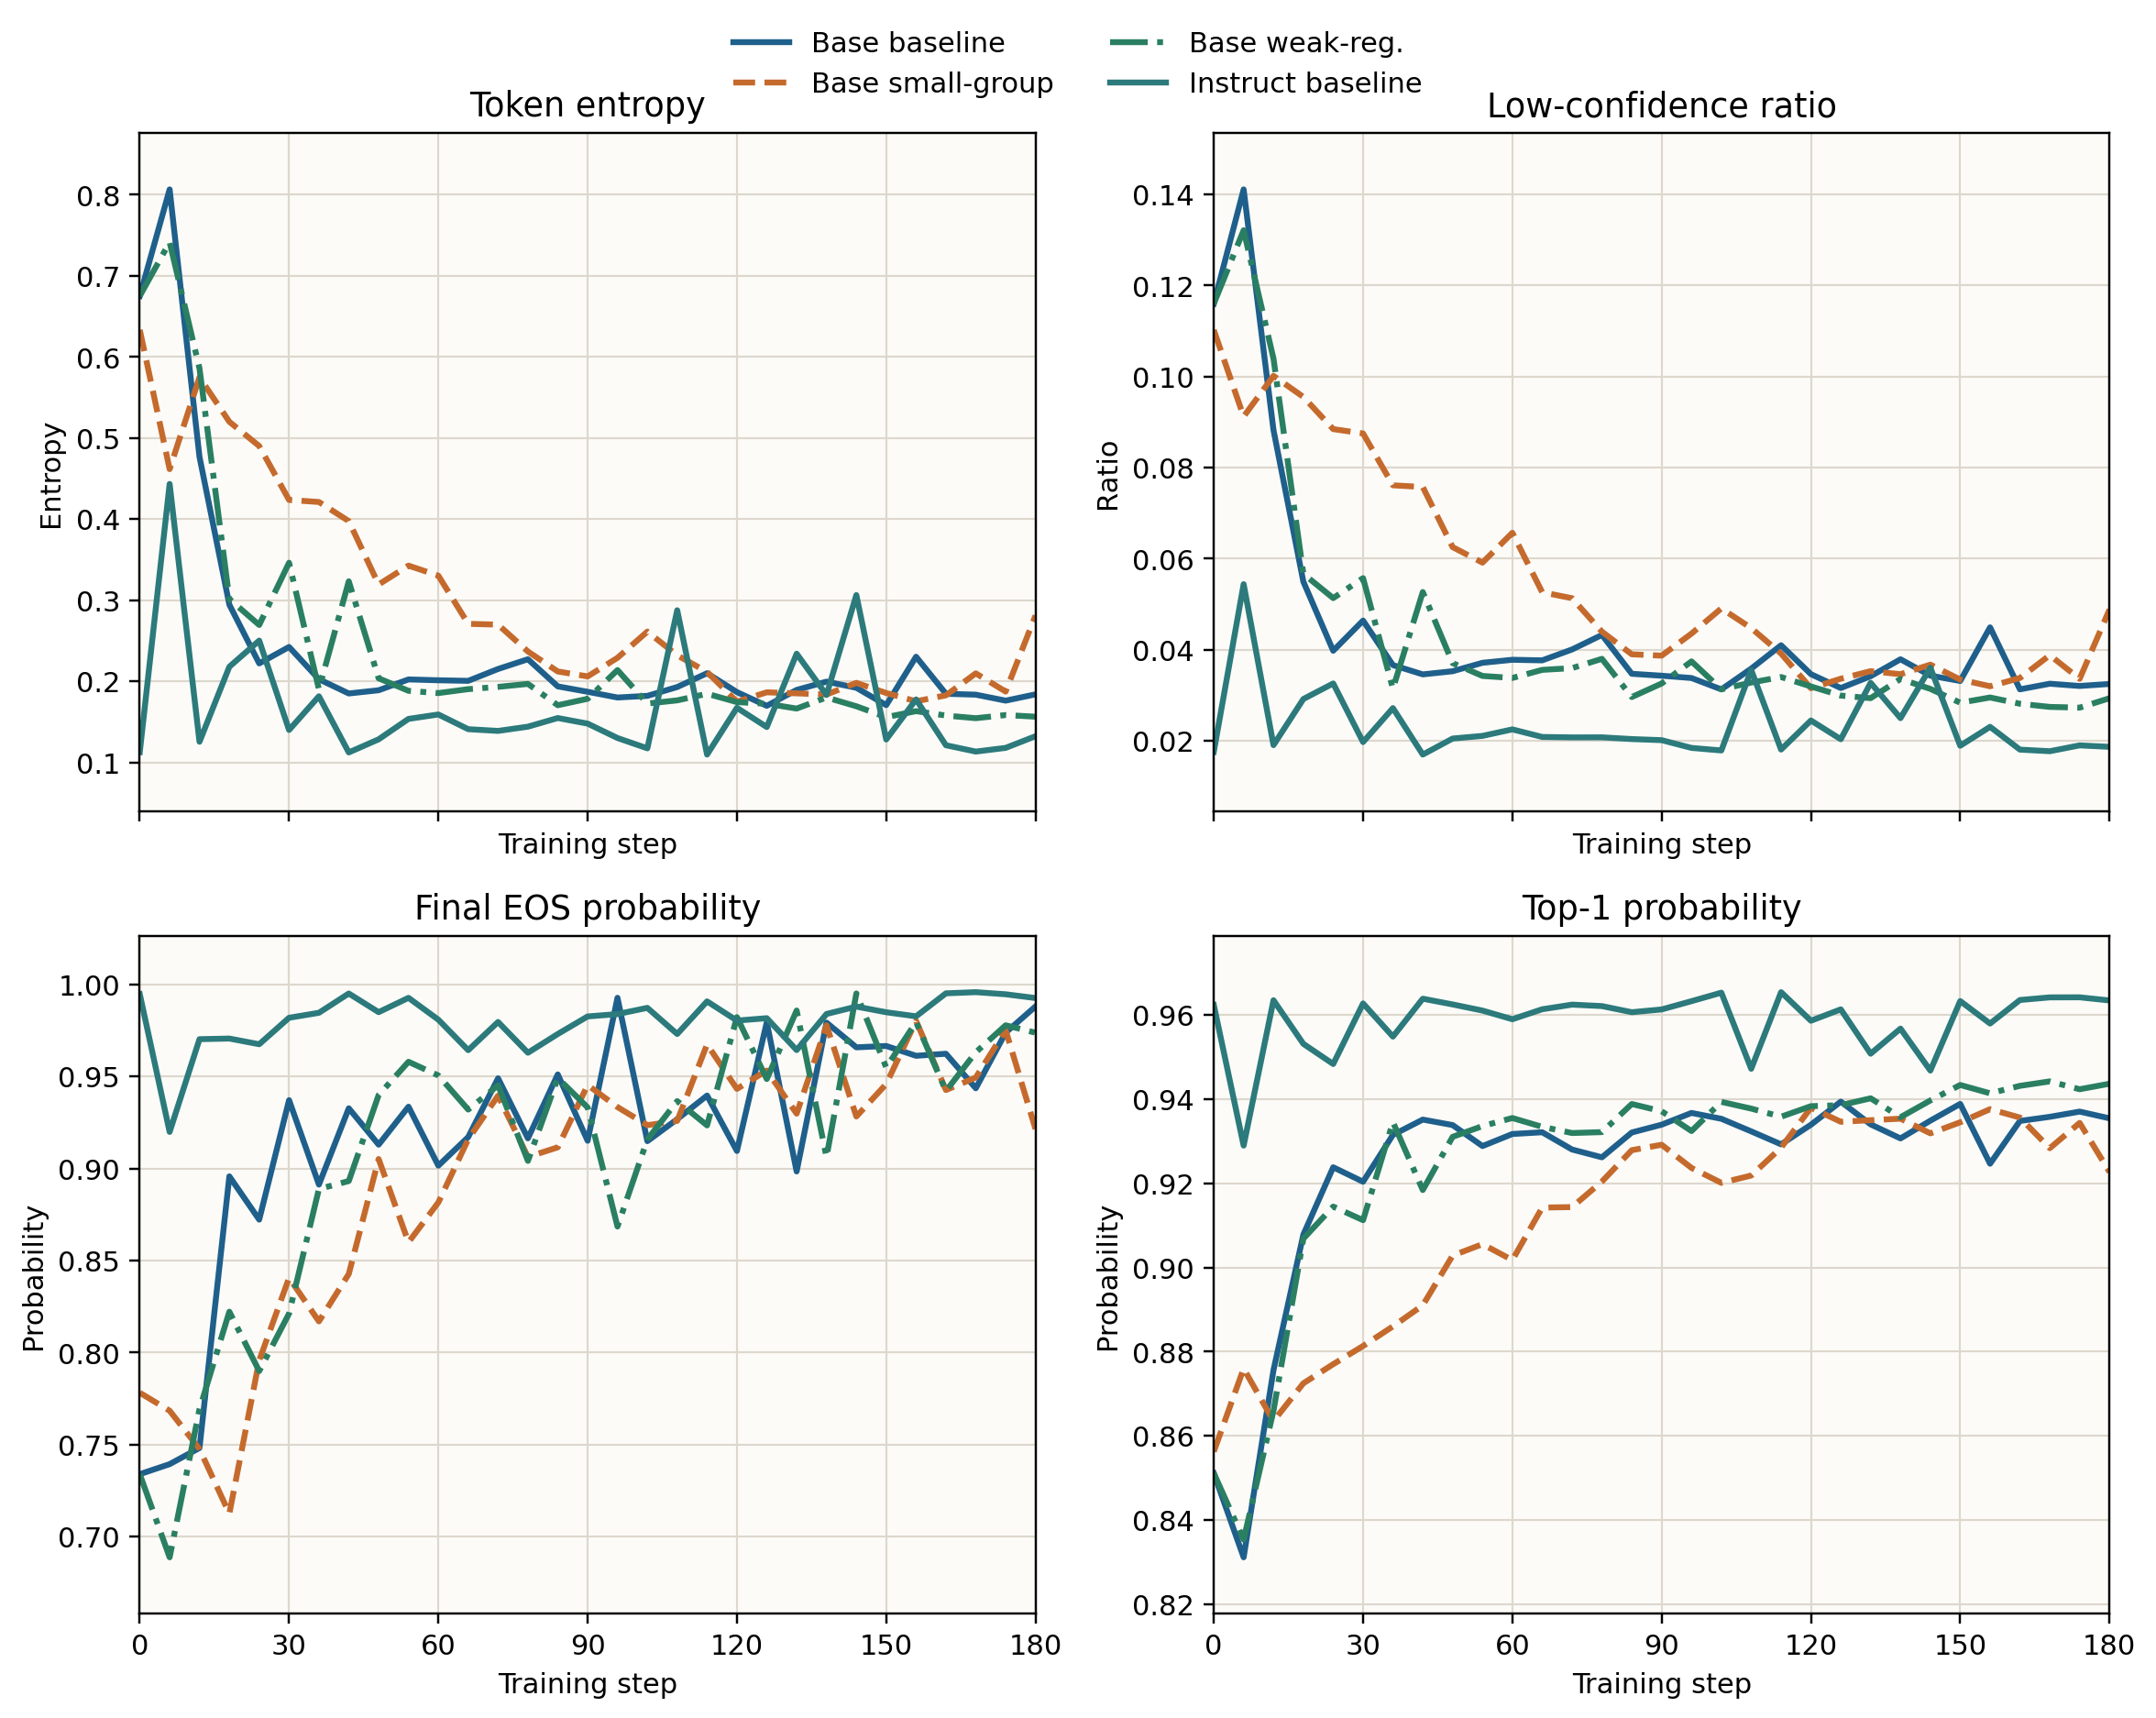
\includegraphics[width=\textwidth]{behavior-detail-noncollapse-panel.png}
    \caption{Fine-grained behavioral dynamics for the four non-collapse conditions.}
    \label{fig:en-behavior-detail-noncollapse}
\end{figure}

If the random-reward setting is kept on the same axes, many of the successful-condition differences become visually compressed. Figure~\ref{fig:en-behavior-detail-noncollapse} therefore removes the collapse case and focuses on the four non-collapse conditions. The zoomed view makes a more nuanced pattern visible: \texttt{Base weak-reg.} exhibits consistently stronger contraction than \texttt{Base n=8}, \texttt{Base n=1} remains weaker on entropy- and confidence-related metrics, and \texttt{Instruct n=8} changes only modestly within an already low-entropy regime.

\subsection{Trajectory-level dynamic summaries}

The dynamic summaries sharpen this interpretation because they move the evidence from static endpoint comparison to trajectory-level mechanism analysis. They compare how training entropy, aggregated validation token entropy, low-confidence ratios, response length, and top-1 probability evolve together, rather than only which condition ends with a slightly higher reward. Table~\ref{tab:en-dynamic-summary} summarizes the start-to-finish changes.

\begin{table}[H]
    \centering
    \caption{Dynamic summary of training and validation diagnostics (start $\rightarrow$ final)}
    \label{tab:en-dynamic-summary}
    \begin{threeparttable}
    \footnotesize
    \setlength{\tabcolsep}{2.6pt}
    \begin{tabularx}{\textwidth}{>{\raggedright\arraybackslash}p{0.24\textwidth}*{5}{>{\centering\arraybackslash}X}}
        \toprule
        Setting & actor ent. & val ent. & low-conf & val len. & top-1 \\
        \midrule
        Base n=8 & 0.346$\rightarrow$0.116 & 0.660$\rightarrow$0.202 & 0.115$\rightarrow$0.037 & 812.5$\rightarrow$603.1 & 0.854$\rightarrow$0.932 \\
        Base n=1 & 0.641$\rightarrow$0.085 & 0.532$\rightarrow$0.317 & 0.095$\rightarrow$0.051 & 762.8$\rightarrow$580.4 & 0.873$\rightarrow$0.921 \\
        Base weak-reg. & 0.346$\rightarrow$0.091 & 0.660$\rightarrow$0.156 & 0.115$\rightarrow$0.030 & 812.5$\rightarrow$578.6 & 0.854$\rightarrow$0.944 \\
        Base random-reward & 0.376$\rightarrow$11.594 & 0.633$\rightarrow$11.547 & 0.110$\rightarrow$1.000 & 762.8$\rightarrow$1192.4 & 0.856$\rightarrow$0.002 \\
        Instruct n=8 & 0.118$\rightarrow$0.062 & 0.111$\rightarrow$0.156 & 0.017$\rightarrow$0.022 & 473.2$\rightarrow$470.3 & 0.964$\rightarrow$0.961 \\
        \bottomrule
    \end{tabularx}
    \begin{tablenotes}[flushleft]
        \footnotesize
        \item Note: the start point is the first checkpoint with a valid value, and the end point is the final validation checkpoint. The validation token metrics come from aggregated token diagnostics with 64 analyzed samples per validation checkpoint, corresponding to about 1.6\% of validation cases.
    \end{tablenotes}
    \end{threeparttable}
\end{table}

\begin{figure}[H]
    \centering
    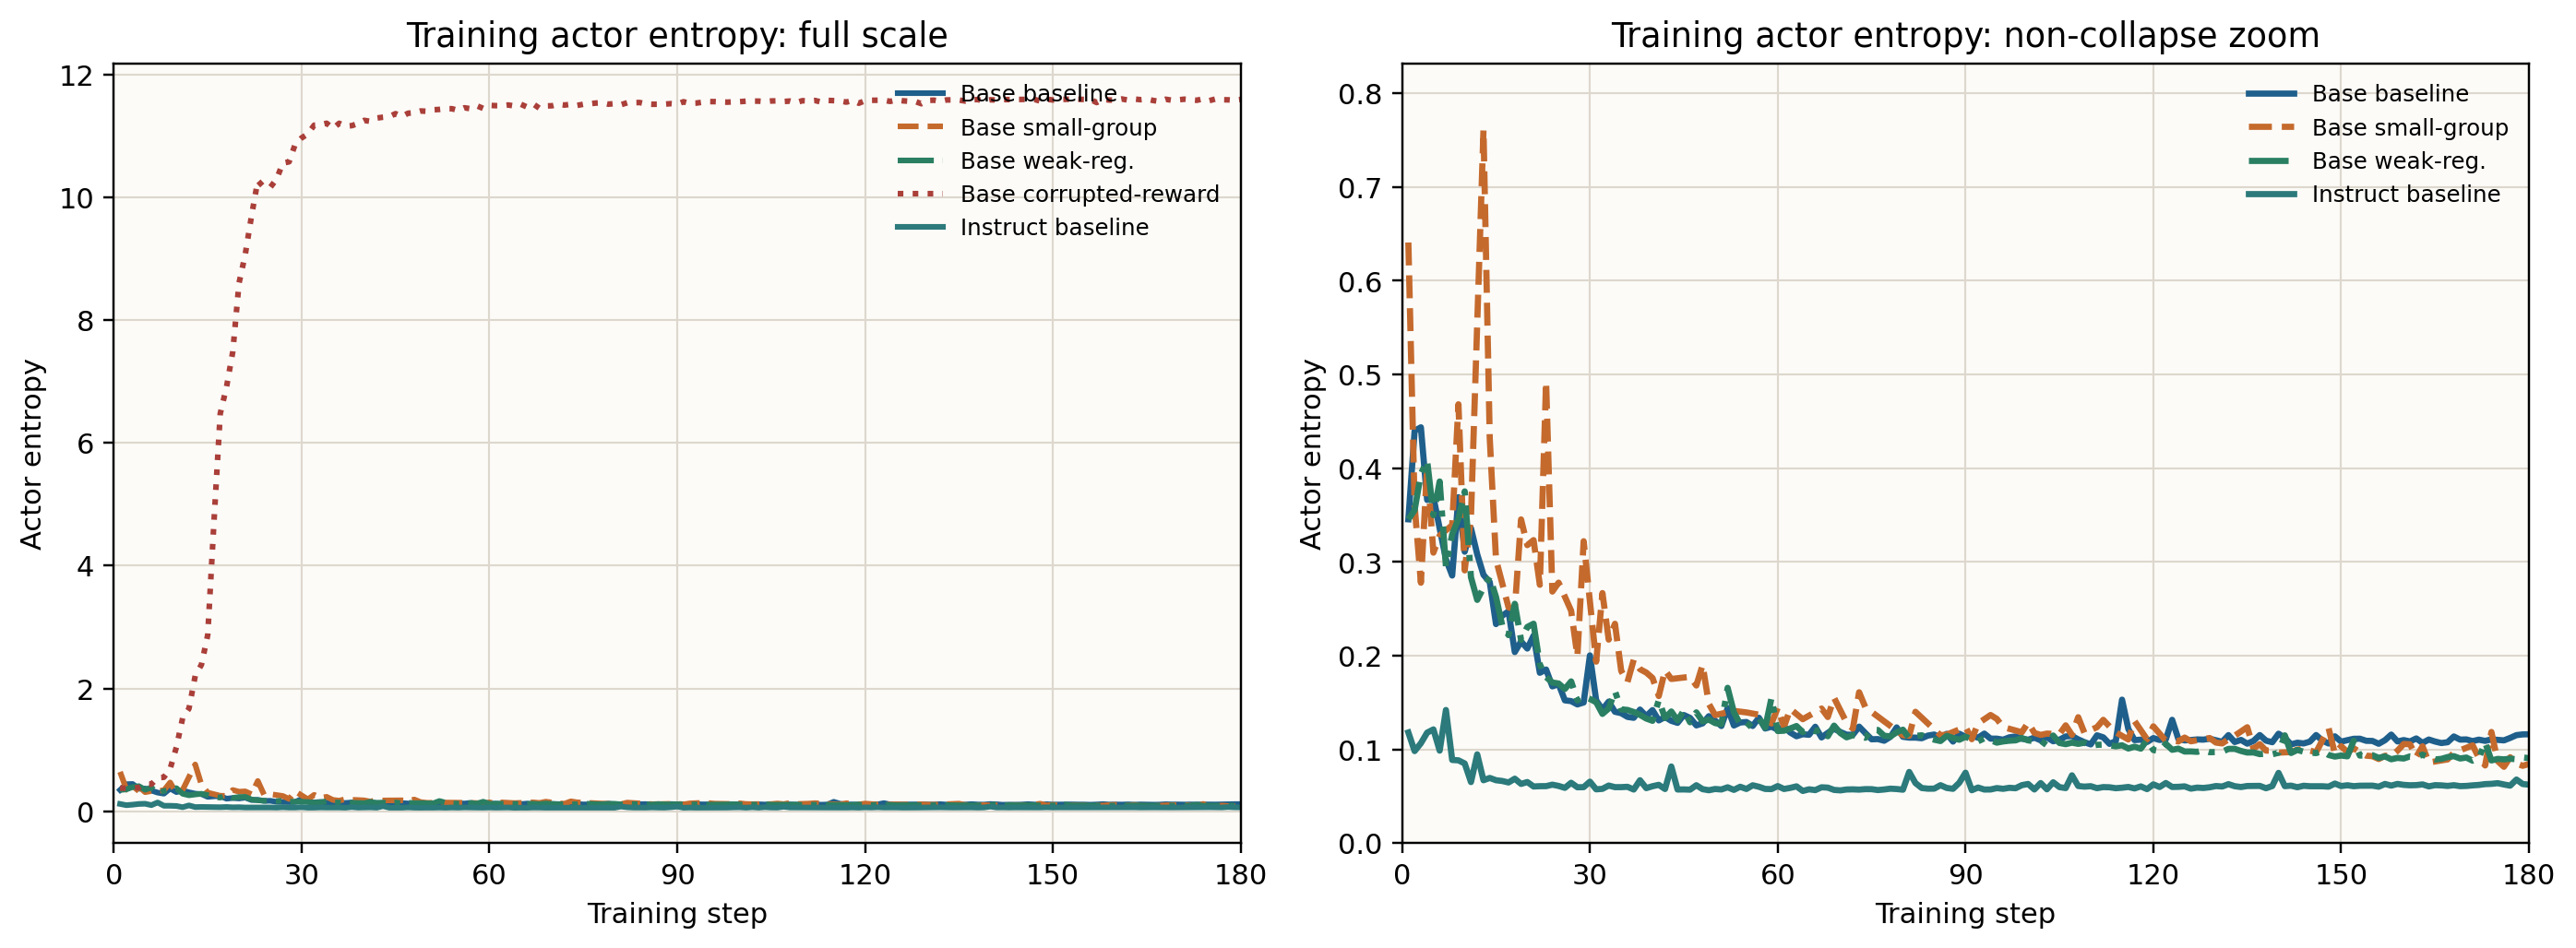
\includegraphics[width=\textwidth]{actor-entropy-static.png}
    \caption{Training-time \texttt{actor/entropy} trajectories for the five diagnostic settings, shown with full-scale and zoomed views.}
    \label{fig:en-actor-entropy}
\end{figure}

\begin{figure}[H]
    \centering
    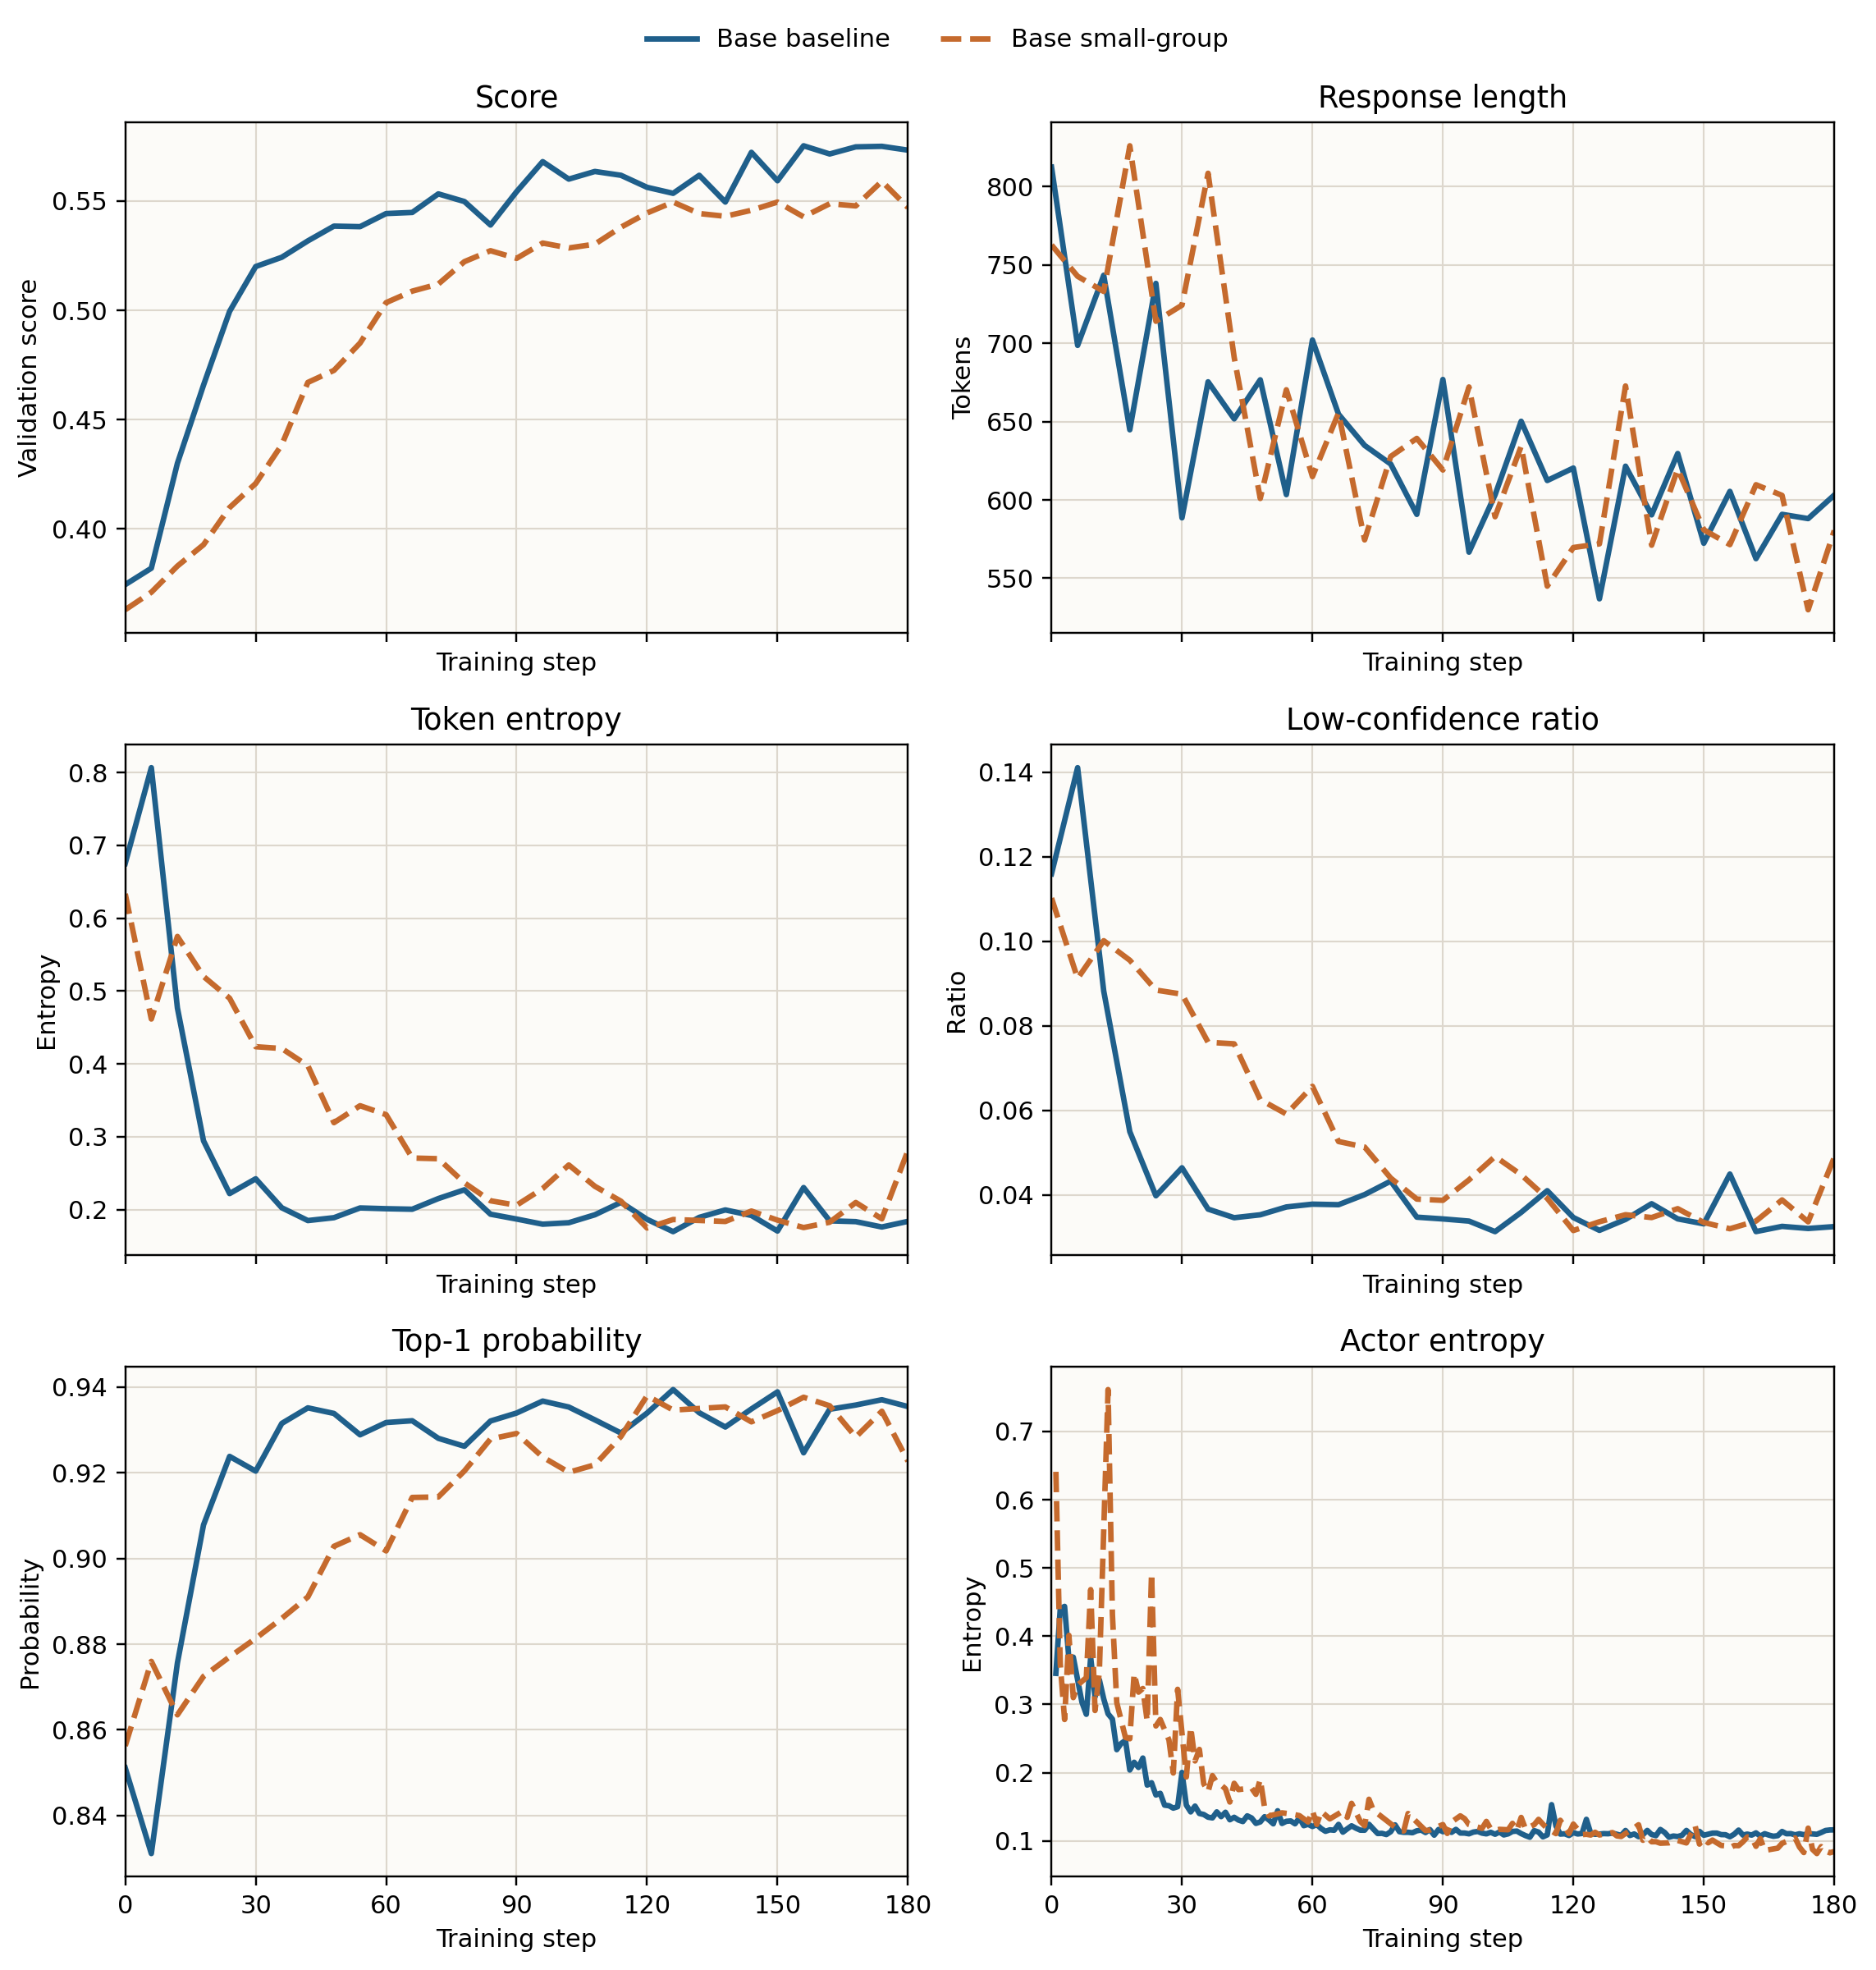
\includegraphics[width=\textwidth]{n1-vs-n8-panel.png}
    \caption{Matched-protocol comparison between \texttt{Base n=8} and \texttt{Base n=1} across six dynamics.}
    \label{fig:en-n1-vs-n8}
\end{figure}

The strongest signal is again the asymmetry between the Base and Instruct families. For \texttt{Base n=8}, \texttt{actor/entropy} drops from 0.346 to 0.116, validation token entropy drops from 0.660 to 0.202, the low-confidence ratio falls from 0.115 to 0.037, aggregated top-1 probability rises from 0.854 to 0.932, and validation response length contracts from 812.5 to 603.1. \texttt{Base weak-reg.} is even more aggressive, ending at 0.091 actor entropy, 0.156 validation token entropy, and 0.944 top-1 probability. This is stronger evidence than score alone for the claim that the Base-family gains come from stabilization and recalibration rather than from merely producing longer or more forceful outputs.

\texttt{Base n=1} provides a sharper and more informative nuance. Under the matched validation protocol, it improves from 0.363 to 0.547, with a best score of 0.559 at step 174. Thus, reducing the training group size from 8 to 1 still leaves substantial learning signal, but the condition remains below \texttt{Base n=8} by about 0.026 at the final checkpoint and about 0.016 at the best checkpoint. Its final validation token entropy is 0.317, well above the 0.202 of \texttt{Base n=8} and the 0.156 of \texttt{Base weak-reg.}; its final low-confidence ratio is 0.051; and its final top-1 probability is only 0.921. Figure~\ref{fig:en-n1-vs-n8} shows that this is not a single-endpoint coincidence but a persistent gap across score, entropy, response length, and top-1 probability. Therefore, reducing group size to one does not prevent learning, but it weakens the quality of stabilization and distributional refinement.

The Instruct family shows the opposite pattern. \texttt{Instruct n=8} changes only modestly: \texttt{actor/entropy} falls from 0.118 to 0.062, validation length is nearly unchanged, and top-1 probability stays around 0.96. This is local refinement rather than structural reorganization. Once the prior is already strong, the current one-shot RL budget mainly smooths an already competent distribution instead of triggering a large behavioral transition.

\subsection{Implications of weak regularization}

\texttt{Base weak-reg.} is especially informative because it ends with a score similar to \texttt{Base n=8} while exhibiting even sharper distributional contraction in some metrics. This does not by itself make the KL and entropy terms unnecessary, but it shows that the final score alone does not capture the full training process. A condition can reach a similar endpoint while traversing a riskier or more aggressive trajectory.

This result should therefore be interpreted through both score and behavior, not through aggregate means alone. The present evidence indicates that removing those constraints did not produce a clear degradation in final accuracy; it does not show that the constraints are irrelevant.

\subsection{The Instruct-family regime}

The Instruct family already begins in a relatively low-entropy and high-confidence region, which explains the smaller movement in the behavioral metrics. There is no comparable transition from ``messy and uncertain'' to ``stable and decisive,'' because the starting point is already close to the latter state. The Instruct setting therefore resembles local refinement, whereas the Base settings exhibit a more substantial stabilization process.

\subsection{Token-level supplementary evidence}

\subsubsection{Scope and limitations of the token-level trace set}

The token-diagnostics analysis uses a fixed prompt and a narrower trace set. Up to 64 samples per checkpoint contribute to the diagnostic statistics, but only 8 samples retain the full token trace, and each trace keeps only roughly the first 96 tokens. The token-level analysis should therefore be interpreted as mechanism-oriented evidence on a fixed trace set, not as a benchmark-wide token statistic.

Even with that limitation, the token-level trace set is highly valuable because it captures quantities such as token entropy, log-probability, top-1 probability, and top-k mass at the token level. These are precisely the quantities needed to test whether training is reorganizing early-token behavior. The paper therefore uses two layers of token evidence: seven-setting aggregate token summaries, which support broad directional and matched full-data claims, and fixed-prompt traces, which support finer-grained mechanism inspection.

\begin{figure}[H]
    \centering
    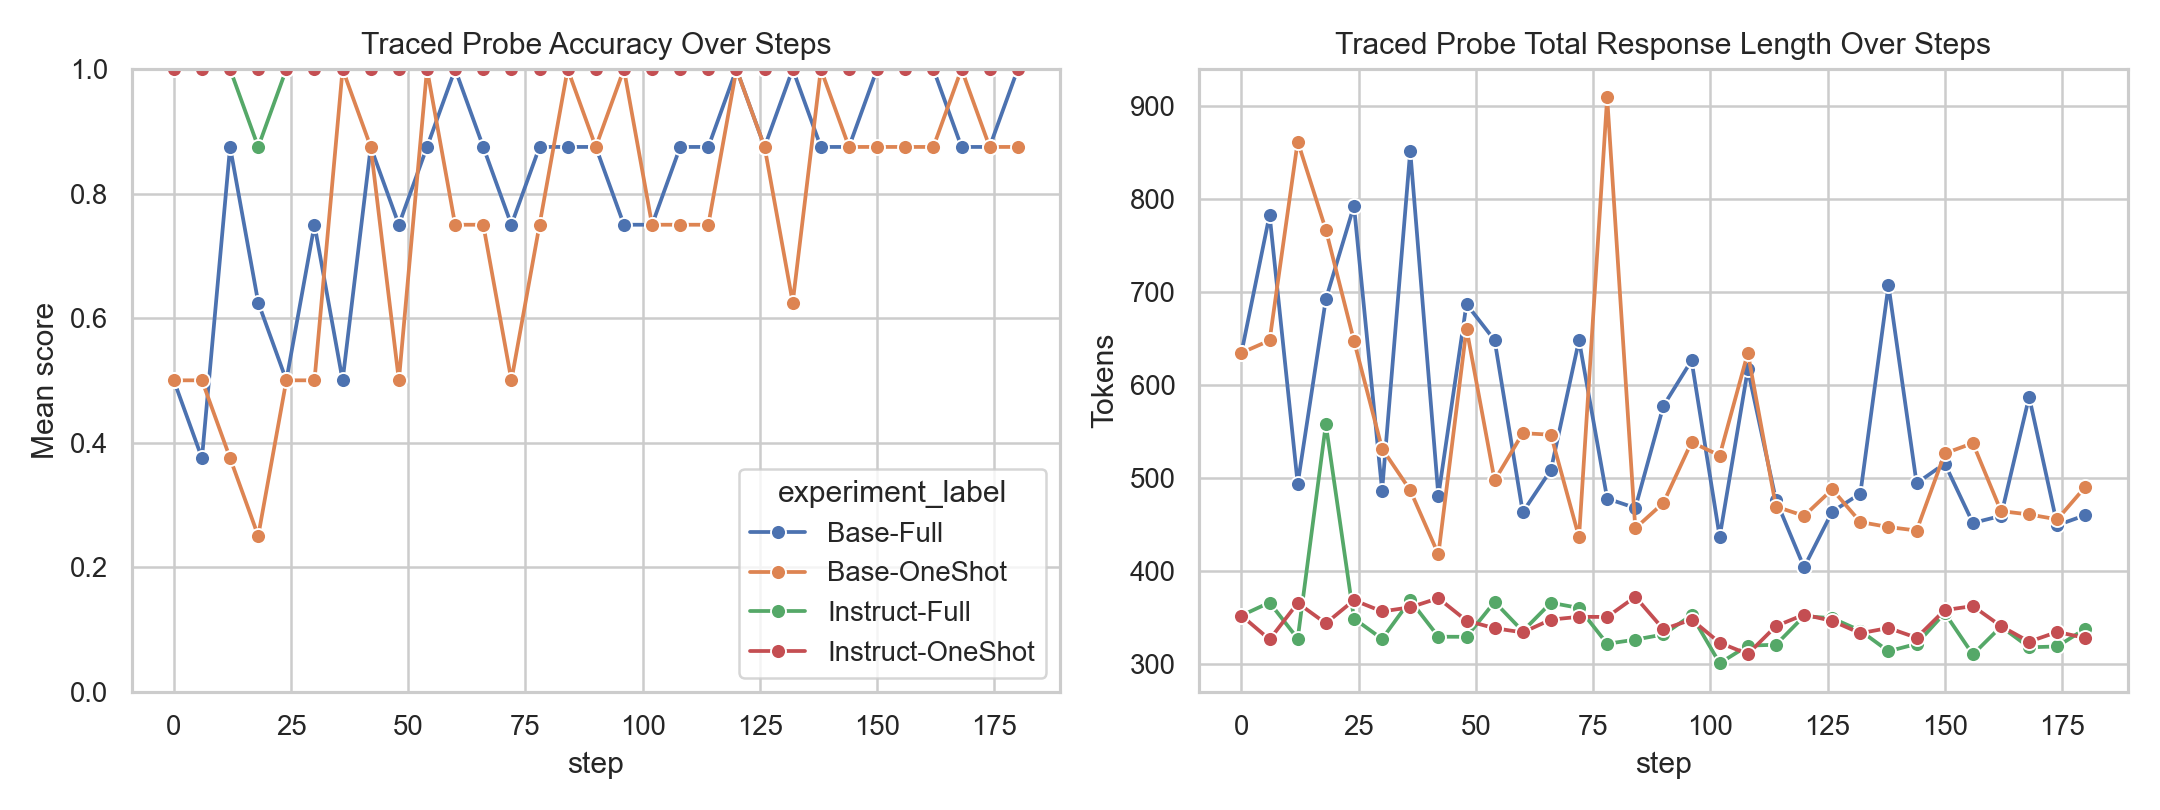
\includegraphics[width=\textwidth]{token-probe-over-steps.png}
    \caption{Fixed-prompt traced outputs across training checkpoints. The figure visualizes how prefix behavior and stopping structure evolve.}
    \label{fig:en-token-steps}
\end{figure}

\subsubsection{Fixed-prompt trace evidence}

The fixed-prompt traces mirror the aggregate results. The Instruct conditions start with higher confidence and lower entropy, and their changes are comparatively small. The Base conditions undergo much larger shifts in log-probability and entropy, especially in the early token region. This provides qualitative support for the claim that Base-model training reduces prefix instability and makes the model converge on a more stable trajectory sooner.

\begin{figure}[t]
    \centering
    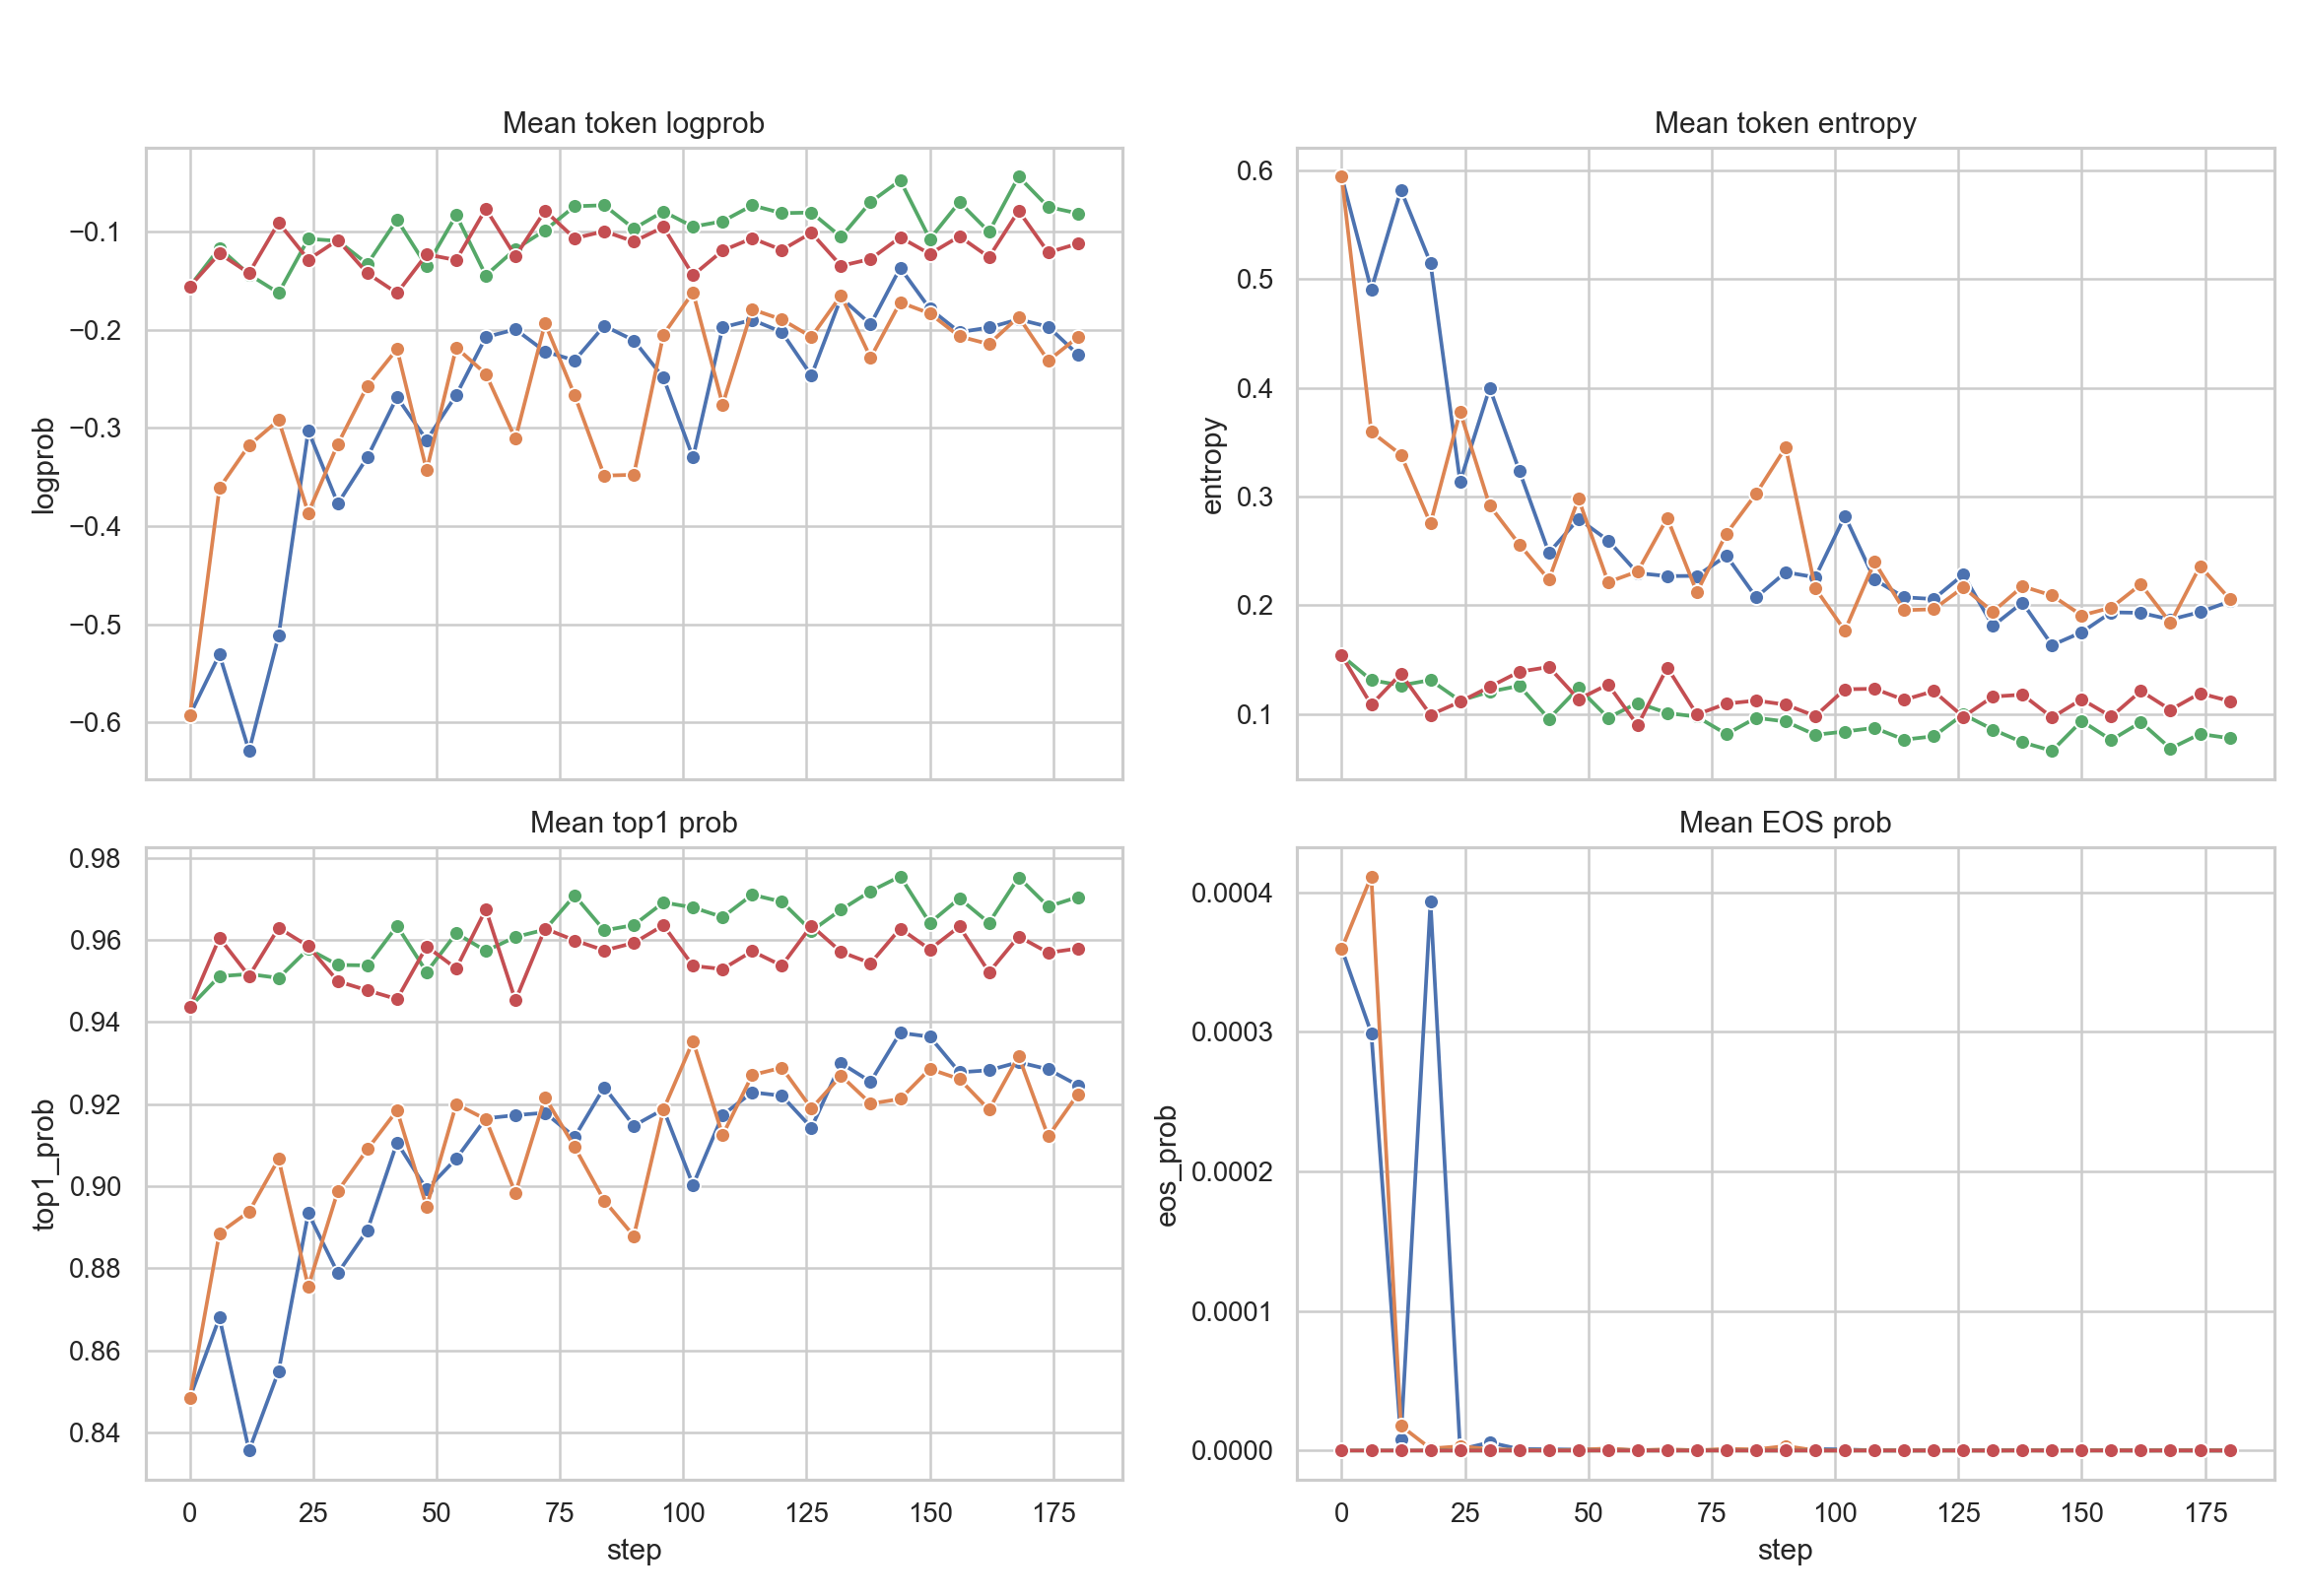
\includegraphics[width=\textwidth]{token-step-metrics.png}
    \caption{Token-level metrics across checkpoints. The figure is narrow in scope but informative about confidence structure and entropy reduction.}
    \label{fig:en-token-metrics}
\end{figure}

\begin{table}[H]
    \centering
    \caption{Final-checkpoint token-level summary on the fixed prompt}
    \label{tab:en-token-final}
    \begin{tabular}{lccccc}
        \toprule
        Setting & correct & traced tokens & entropy & top1 prob & top5 mass \\
        \midrule
        Base-Full & correct & 768 & 0.2036 & 0.9246 & 0.9970 \\
        Base-OneShot & correct & 672 & 0.2005 & 0.9248 & 0.9970 \\
        Base-OneShot & wrong & 96 & 0.2435 & 0.9056 & 0.9977 \\
        Instruct-Full & correct & 768 & 0.0778 & 0.9705 & 0.9998 \\
        Instruct-OneShot & correct & 768 & 0.1119 & 0.9580 & 0.9996 \\
        \bottomrule
    \end{tabular}
\end{table}

\begin{table}[H]
    \centering
    \caption{Token-level deltas from step 0 to the final checkpoint on the fixed prompt}
    \label{tab:en-token-delta}
    \begin{tabular}{lccc}
        \toprule
        Setting & $\Delta$ logprob & $\Delta$ entropy & $\Delta$ top1 prob \\
        \midrule
        Base-Full & +0.3673 & -0.3908 & +0.0762 \\
        Base-OneShot & +0.3849 & -0.3885 & +0.0740 \\
        Instruct-Full & +0.0744 & -0.0760 & +0.0268 \\
        Instruct-OneShot & +0.0435 & -0.0419 & +0.0143 \\
        \bottomrule
    \end{tabular}
\end{table}

The numbers in Tables~\ref{tab:en-token-final} and~\ref{tab:en-token-delta} reinforce that interpretation. The Base settings exhibit substantially larger entropy decreases and larger increases in token confidence than the Instruct settings. This pattern is consistent with 1-shot GRPO acting mainly as a calibration mechanism for the weaker model family, and Figures~\ref{fig:en-token-steps} and~\ref{fig:en-token-metrics} show the same pattern visually.

\subsubsection{Prefix-level reorganization}

The final-answer region is only part of the behavioral evidence. Figure~\ref{fig:en-prefix-curves-main} moves attention to the prefix region of the output distribution at the final checkpoint. Its main value is that it shows the training effect well before the answer is closed. For the Base family, the more stable final outcome is not just an endpoint effect; the early trajectory already looks more structured, lower-entropy, and more concentrated. This observation is important because mathematical reasoning often fails long before the last answer token.

Figure~\ref{fig:en-prefix-curves-main} also complements the aggregate dynamic evidence. The dynamic curves show a consistent contraction over training, while the prefix plot shows that this contraction is visible positionally in the early output as well. The model is therefore not merely becoming more confident at the end; it is entering a more stable reasoning track sooner.

\begin{figure}[H]
    \centering
    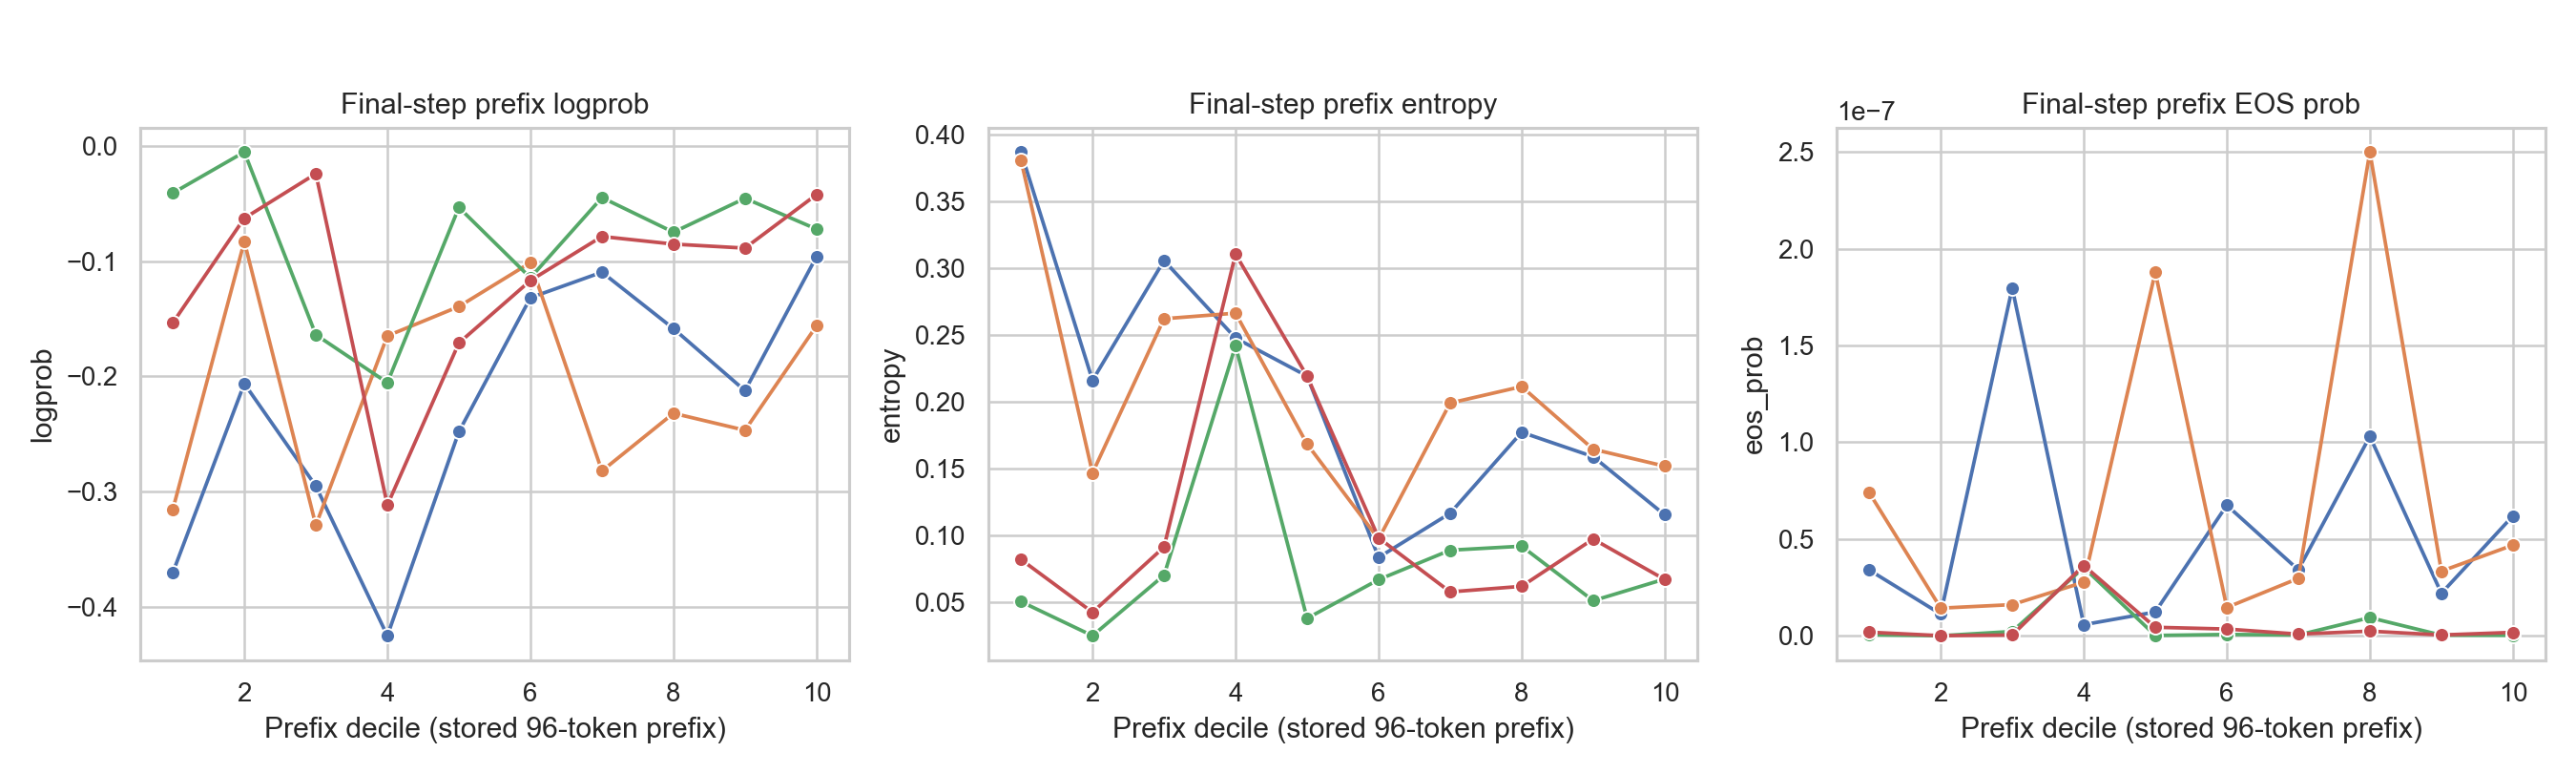
\includegraphics[width=\textwidth]{final-prefix-curves.png}
    \caption{Prefix-region curves at the final checkpoint. The figure shows that the training effect is already visible early in the generated trajectory, not only near the final answer.}
    \label{fig:en-prefix-curves-main}
\end{figure}

\subsubsection{Local contraction from the initial to final checkpoint}

Figure~\ref{fig:en-token-delta-main} focuses on the before-after delta itself. This makes it especially useful for distinguishing broad small improvements from substantial probability-mass redistribution in specific token regions. The figure strongly favors the latter interpretation for the Base conditions. The changes in log-probability and entropy are much larger than in the Instruct conditions, especially in the early and middle token regions.

This also helps frame \texttt{Base n=1} more carefully. The fixed-prompt trace set was not built specifically for that setting, so it is not a direct visualization of that setting. However, the mode of change it reveals matches the aggregate pattern: Base-model training can produce more concentrated token distributions, and reducing group size preserves that process only partially rather than fully.

\begin{figure}[H]
    \centering
    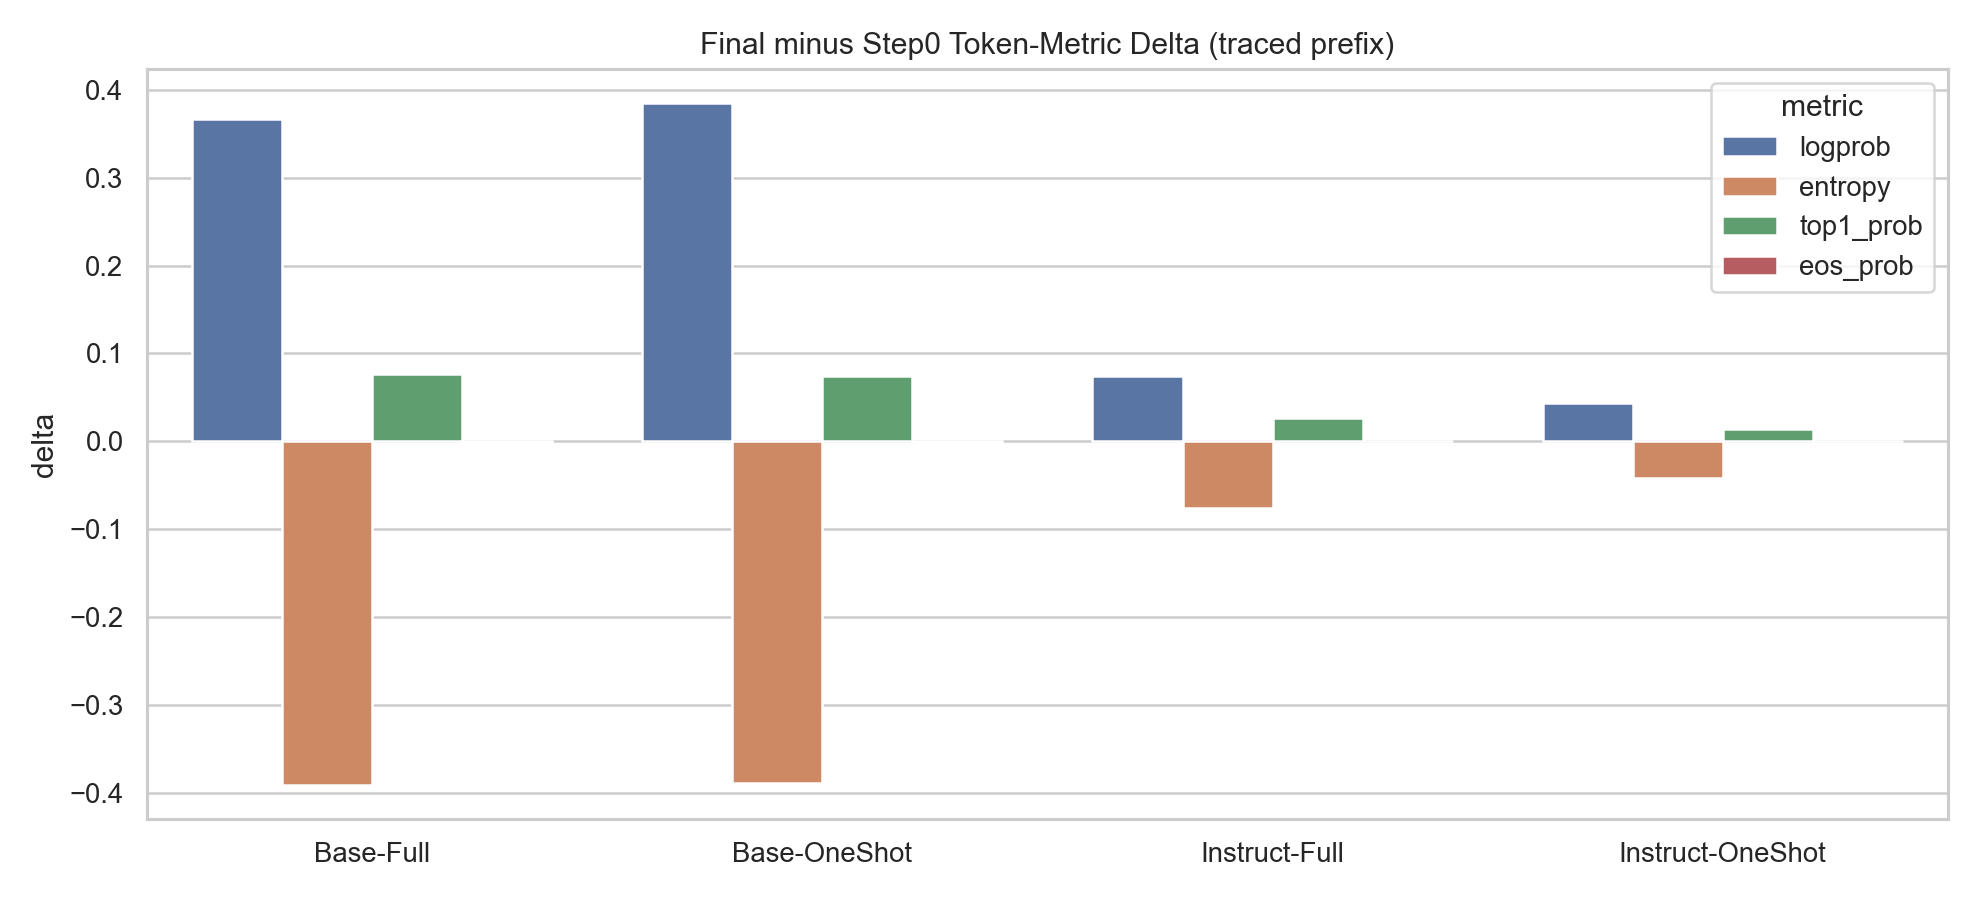
\includegraphics[width=\textwidth]{token-delta-step0-to-final.png}
    \caption{Token-level deltas from the initial to final checkpoint.}
    \label{fig:en-token-delta-main}
\end{figure}

\subsubsection{Correctness-conditioned distribution separation}

To test whether distributional contraction is genuinely related to task success, we group the validation records with retained token-diagnostics summaries by response correctness and compare mean token entropy with mean top-1 probability. Figure~\ref{fig:en-correct-wrong-support-panel} summarizes the final-checkpoint 64-sample diagnostics from the six non-collapse settings and tracks correctness-conditioned gaps for the matched one-shot/full-data pairs in both model families. The main result is consistent: correct responses systematically occupy the more contracted side of the distribution, with lower entropy and higher top-1 concentration.

This separation is visible across all six non-collapse conditions at the final checkpoint. The correct/wrong mean token entropies are 0.165/0.237 for \texttt{Base n=8}, 0.162/0.209 for \texttt{Base full-data}, 0.159/0.570 for \texttt{Base n=1}, 0.152/0.172 for \texttt{Base weak-reg.}, 0.087/0.499 for \texttt{Instruct n=8}, and 0.074/0.163 for \texttt{Instruct full-data}. The corresponding mean top-1 probabilities are 0.939/0.925, 0.940/0.929, 0.941/0.878, 0.945/0.940, 0.968/0.925, and 0.972/0.967. The magnitude of the separation varies by condition, but its direction is unchanged. The contraction and confidence concentration documented throughout the paper are therefore not merely cosmetic properties of the token distribution; they are stably associated with successful problem solving.

The checkpoint-wise grouped statistics further show that this relationship is not confined to the terminal checkpoint. In the bottom row of Figure~\ref{fig:en-correct-wrong-support-panel}, the entropy gap is defined as wrong minus correct, and the top-1 gap is defined as correct minus wrong. For the Base family, \texttt{Base n=8} and \texttt{Base full-data} share the same initial gap at \texttt{step 0}; at the final checkpoint, their entropy gaps are 0.072 and 0.047, and their top-1 gaps are 0.0149 and 0.0105. For the Instruct family, \texttt{Instruct n=8} and \texttt{Instruct full-data} end with entropy gaps of 0.412 and 0.089 and top-1 gaps of 0.0429 and 0.0047. The correctness-conditioned distribution gap therefore persists across matched one-shot/full-data comparisons rather than emerging only in a small traced subset at the end. \texttt{Base random-reward} is excluded from this figure because it has no correct responses at the final checkpoint.

This section answers the mechanism question at two levels. Aggregate behavioral metrics show the broad stabilization pattern, while token-level traces show that the same change is visible inside generated trajectories. The evidence therefore supports the calibration account without requiring the reader to treat each diagnostic as an isolated result.

\IfFileExists{sections/full_token_ckpt_analysis_en.tex}{%
\subsection{Offline full-token checkpoint audit}

The retained training-time token traces are useful for mechanism inspection, but they have two important limits: they are narrow retained traces, and the detailed token fields only cover an early response prefix. The saved-checkpoint audit tests whether the same stabilization pattern survives when checkpoints are reloaded directly. The audit restores the saved actor checkpoints, regenerates responses on a fixed held-out subset of \EvalSet{}, and scores every generated response token rather than only the first retained prefix tokens.

The audit covers checkpoint step 0 through step 180. For each checkpoint, it evaluates 32 held-out problems with 128 sampled responses in total. This is still a subset audit rather than a replacement for the full validation curve, but it is stricter than the earlier fixed-prompt trace view because the token statistics are recomputed from the saved checkpoints over complete generated sequences.

\begin{table}[H]
    \centering
    \caption{Offline full-token audit across saved checkpoints}
    \label{tab:en-full-token-ckpt-audit}
    \small
    \setlength{\tabcolsep}{4pt}
    \begin{tabular}{rrrrrrr}
        \toprule
        Step & score & length & entropy & low-conf. & top-1 & tail conf. \\
        \midrule
        0 & 0.3047 & 812.1 & 0.6982 & 0.1254 & 0.8385 & 0.7755 \\
        60 & 0.6172 & 609.9 & 0.2394 & 0.0452 & 0.9184 & 0.9220 \\
        120 & 0.5859 & 608.9 & 0.2710 & 0.0492 & 0.9149 & 0.9066 \\
        180 & 0.6172 & 662.9 & 0.2188 & 0.0398 & 0.9256 & 0.9066 \\
        \bottomrule
    \end{tabular}
\end{table}

The checkpoint-level pattern is directionally consistent with the broader calibration account. From step 0 to step 180, score changes by 0.3125, average response length changes by -149.2 tokens, mean token entropy changes by -0.4794, the low-confidence-token ratio changes by -0.0856, and mean top-1 probability changes by 0.0871. The best score in this audit is 0.6172 at step 60, so the saved-checkpoint view again warns against reading the last checkpoint as the only meaningful endpoint.

The largest behavioral transition happens early, between the base model and step 60. Over this interval, score rises from 0.3047 to 0.6172, average length falls from 812.1 to 609.9 tokens, entropy falls from 0.6982 to 0.2394, low-confidence mass falls from 0.1254 to 0.0452, and mean top-1 probability rises from 0.8385 to 0.9184. This is the cleanest full-response evidence for the calibration interpretation: the gain is not produced by longer exploration, but by shorter and more concentrated generations with fewer low-confidence tokens.

The later checkpoints add a useful nuance. Steps 60 and 180 tie in score at 0.6172, but they are not behaviorally identical. Step 180 has lower entropy, lower low-confidence mass, and higher mean top-1 probability than step 60, while being about 53 tokens longer on average and having lower tail confidence. Step 120 has nearly the same length as step 60 but a lower score, together with slightly higher entropy and low-confidence mass. These contrasts show why no single token metric should be treated as the whole mechanism. The useful region is a balance among correctness, response economy, confidence, and stable termination.

EOS behavior needs a separate reading. In this audit, the EOS metrics describe the probability assigned to the EOS token at each generated position, and whether EOS enters a high-probability or top-1 region; they are not a direct count of whether a sampled response terminates with EOS. Table~\ref{tab:en-full-token-eos-summary} multiplies the raw ratios by $10^4$ for readability. The main pattern is not a monotonic increase in stopping pressure. Mean EOS probability falls from 2.613 at step 0 to 0.827 at step 60 and 0.098 at step 120, then rebounds to 0.806 at step 180. Final-position EOS probability follows a similar non-monotonic pattern: steps 60 and 120 are far below step 0, while step 180 recovers part of the tail-end EOS mass but remains below the initial checkpoint. Thus the score gain is not explained by a model that simply becomes more eager to stop everywhere. A more careful interpretation is that training first suppresses unnecessary EOS pressure while producing a more stable reasoning trajectory, and the final checkpoint restores some tail-end closure without returning to the initial high-uncertainty regime.

\begin{table}[H]
    \centering
    \caption{EOS behavior in the offline full-token audit (raw ratios $\times 10^4$)}
    \label{tab:en-full-token-eos-summary}
    \small
    \setlength{\tabcolsep}{5pt}
    \begin{tabular}{rrrrr}
        \toprule
        Step & mean EOS & final EOS & EOS $>0.1$ ratio & EOS top-1 ratio \\
        \midrule
        0 & 2.613 & 8.906 & 2.547 & 2.399 \\
        60 & 0.827 & 0.408 & 1.488 & 0.548 \\
        120 & 0.098 & 0.230 & 0.069 & 0.108 \\
        180 & 0.806 & 2.586 & 2.121 & 0.961 \\
        \bottomrule
    \end{tabular}
\end{table}

The correctness-conditioned full-token rows support the same interpretation. At the final checkpoint, token-weighted correct responses have lower entropy than wrong responses (0.1850 vs. 0.2619) and higher mean top-1 probability (0.9345 vs. 0.9156). The sample-level grouping in Table~\ref{tab:en-full-token-correct-wrong-sample-summary} makes the contrast more concrete. At every checkpoint, the correct group is much shorter than the wrong group and also has lower entropy, lower low-confidence-token ratio, higher tail confidence, and higher mean top-1 probability. At the final checkpoint, correct samples average 476.5 tokens while wrong samples average 963.4 tokens; correct-sample entropy is 0.1765 versus 0.2871 for wrong samples; and the low-confidence-token ratio is 0.0301 versus 0.0555. Thus successful full responses are not merely sharper in a token-weighted average; they are shorter, more stable, and more confidently closed at the sample level.

\begin{table}[H]
    \centering
    \caption{Sample-level correct/wrong grouping in the offline full-token audit}
    \label{tab:en-full-token-correct-wrong-sample-summary}
    \scriptsize
    \setlength{\tabcolsep}{3pt}
    \begin{tabular}{rlrrrrrr}
        \toprule
        Step & group & $n$ & length & entropy & low-conf. & tail conf. & top-1 \\
        \midrule
        0 & correct & 39 & 482.4 & 0.3282 & 0.0619 & 0.8875 & 0.8978 \\
        0 & wrong & 89 & 956.5 & 0.8603 & 0.1533 & 0.7264 & 0.8125 \\
        60 & correct & 79 & 482.5 & 0.2231 & 0.0412 & 0.9286 & 0.9229 \\
        60 & wrong & 49 & 815.4 & 0.2657 & 0.0517 & 0.9114 & 0.9112 \\
        120 & correct & 75 & 473.1 & 0.2126 & 0.0388 & 0.9298 & 0.9268 \\
        120 & wrong & 53 & 801.2 & 0.3537 & 0.0639 & 0.8737 & 0.8980 \\
        180 & correct & 79 & 476.5 & 0.1765 & 0.0301 & 0.9381 & 0.9362 \\
        180 & wrong & 49 & 963.4 & 0.2871 & 0.0555 & 0.8559 & 0.9084 \\
        \bottomrule
    \end{tabular}
\end{table}

These grouped results preserve the same direction observed in the aggregate token diagnostics, so the offline audit functions as mechanism evidence rather than only as a visual diagnostic: it extends the correctness-calibration link from retained prefixes to complete generated sequences. It also sharpens the interpretation of EOS. Useful training is not equivalent to raising EOS probability everywhere. Instead, the better checkpoints combine lower entropy, fewer low-confidence tokens, shorter correct responses, and a controlled rather than globally inflated EOS tendency.

The trajectory-level rendering in Figure~\ref{fig:en-trajectory-text-entropy-math500-18} shows the same pattern at the level of readable generated text. The figure follows one held-out MATH500 trajectory across checkpoint steps 0, 60, 120, and 180. Each word-like unit is printed directly, and its background color encodes token entropy. The step-0 response contains many high-entropy regions and an unstable reasoning path; by the final checkpoint, the visible reasoning is more structured, lower-entropy, and correct. The image is intentionally truncated for readability, so it should be read as a qualitative trajectory view rather than as a full response transcript.

\begin{figure}[H]
    \centering
    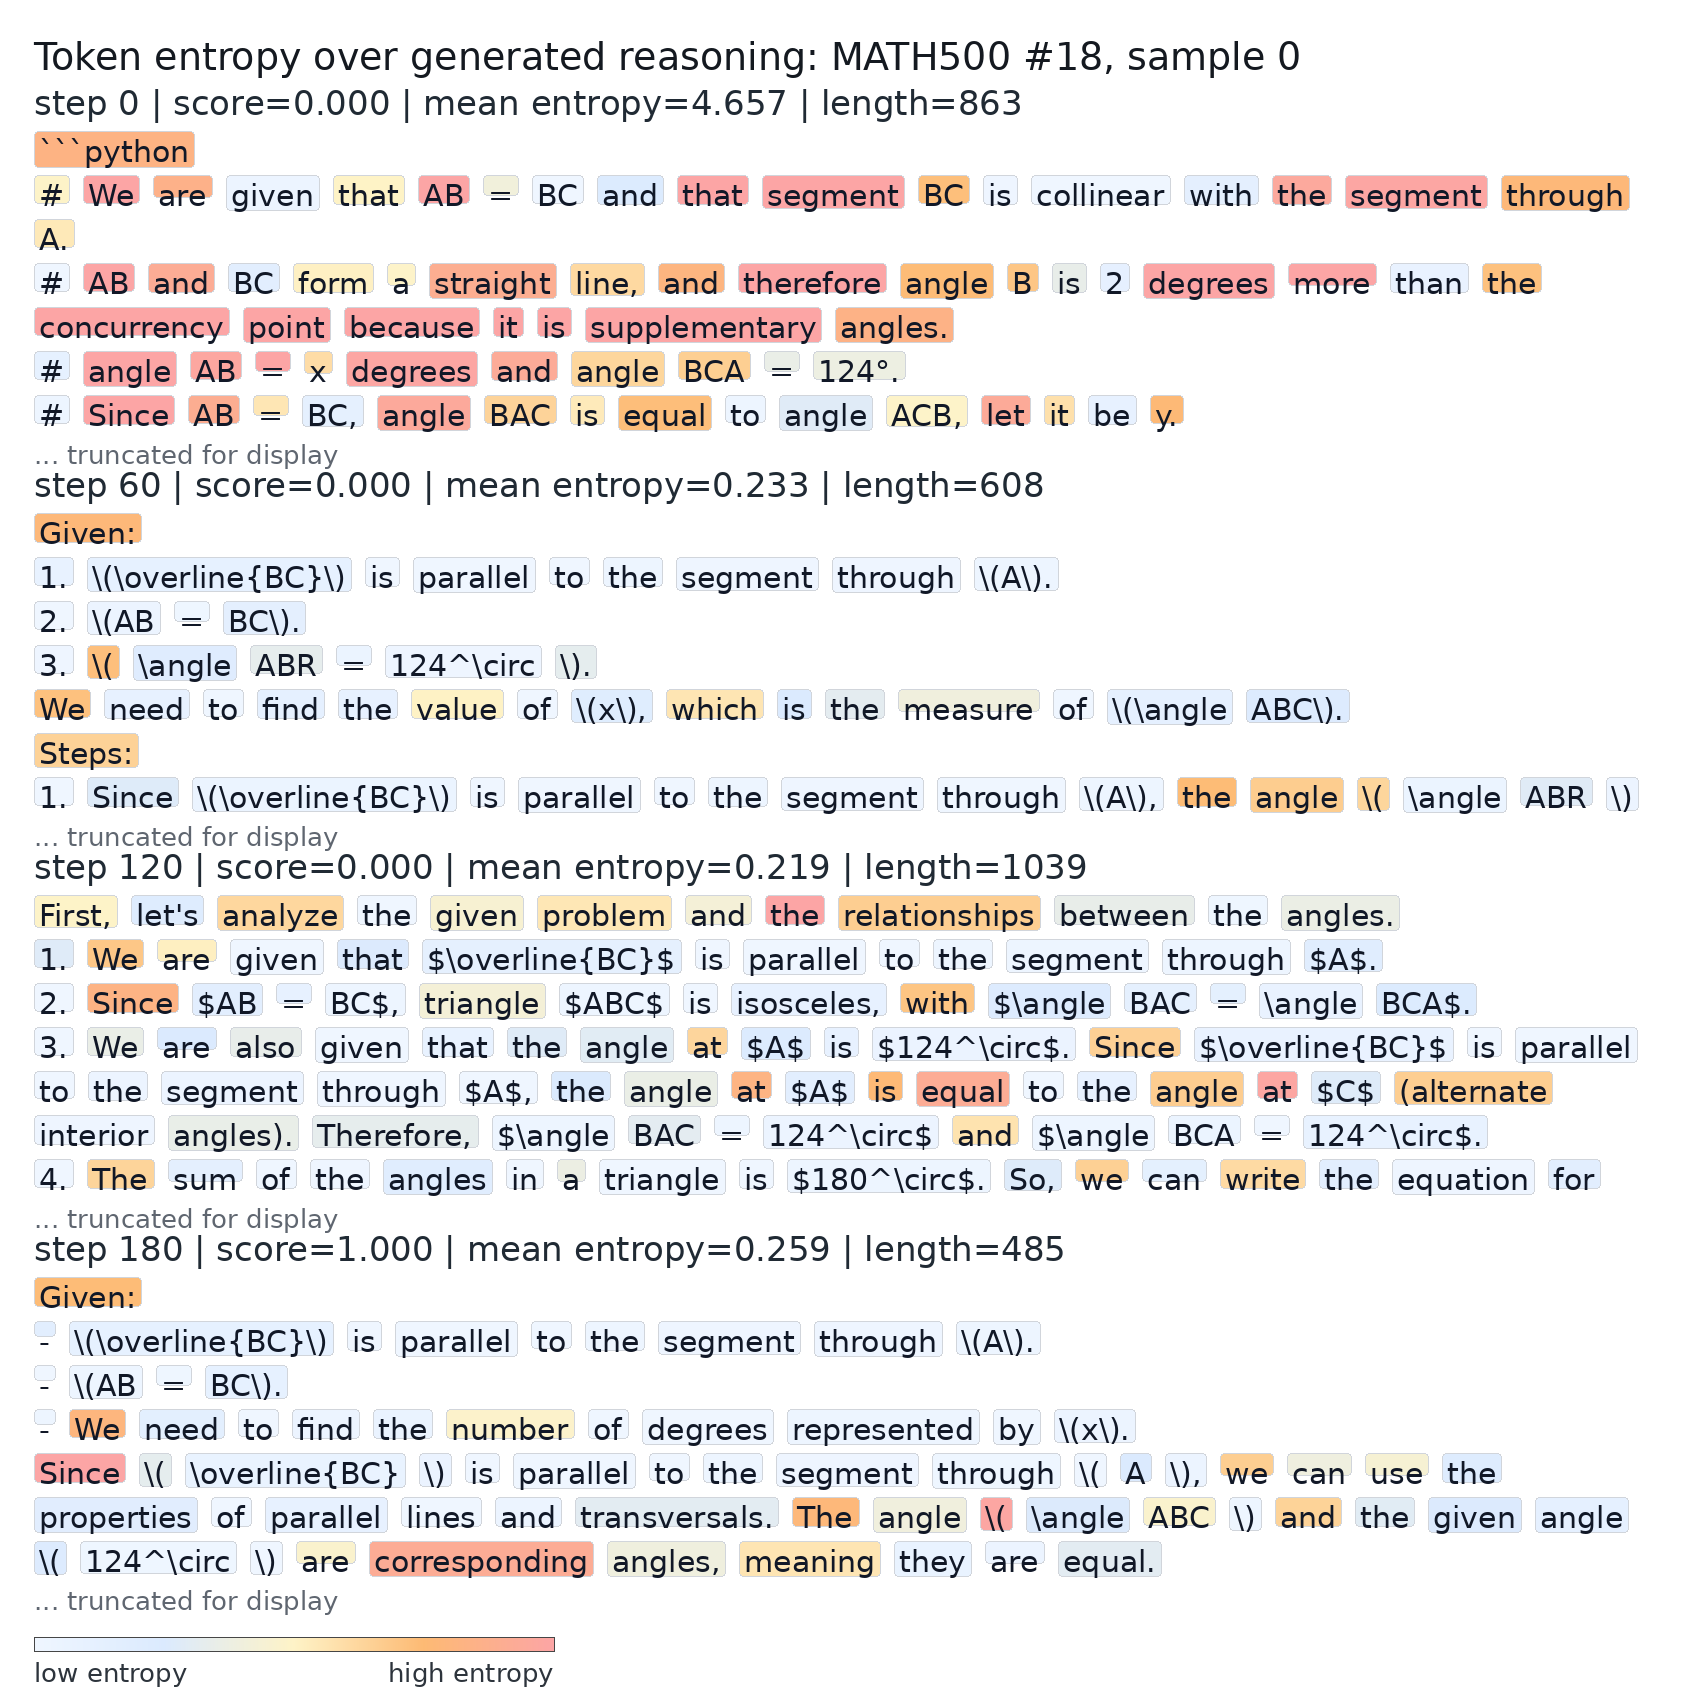
\includegraphics[width=\textwidth]{trajectory-text-entropy-math500-18.png}
    \caption{Representative word-level entropy trajectory across saved checkpoints. Each displayed word or formula fragment is drawn from the generated response, with warmer backgrounds indicating higher token entropy.}
    \label{fig:en-trajectory-text-entropy-math500-18}
\end{figure}

\begin{figure}[H]
    \centering
    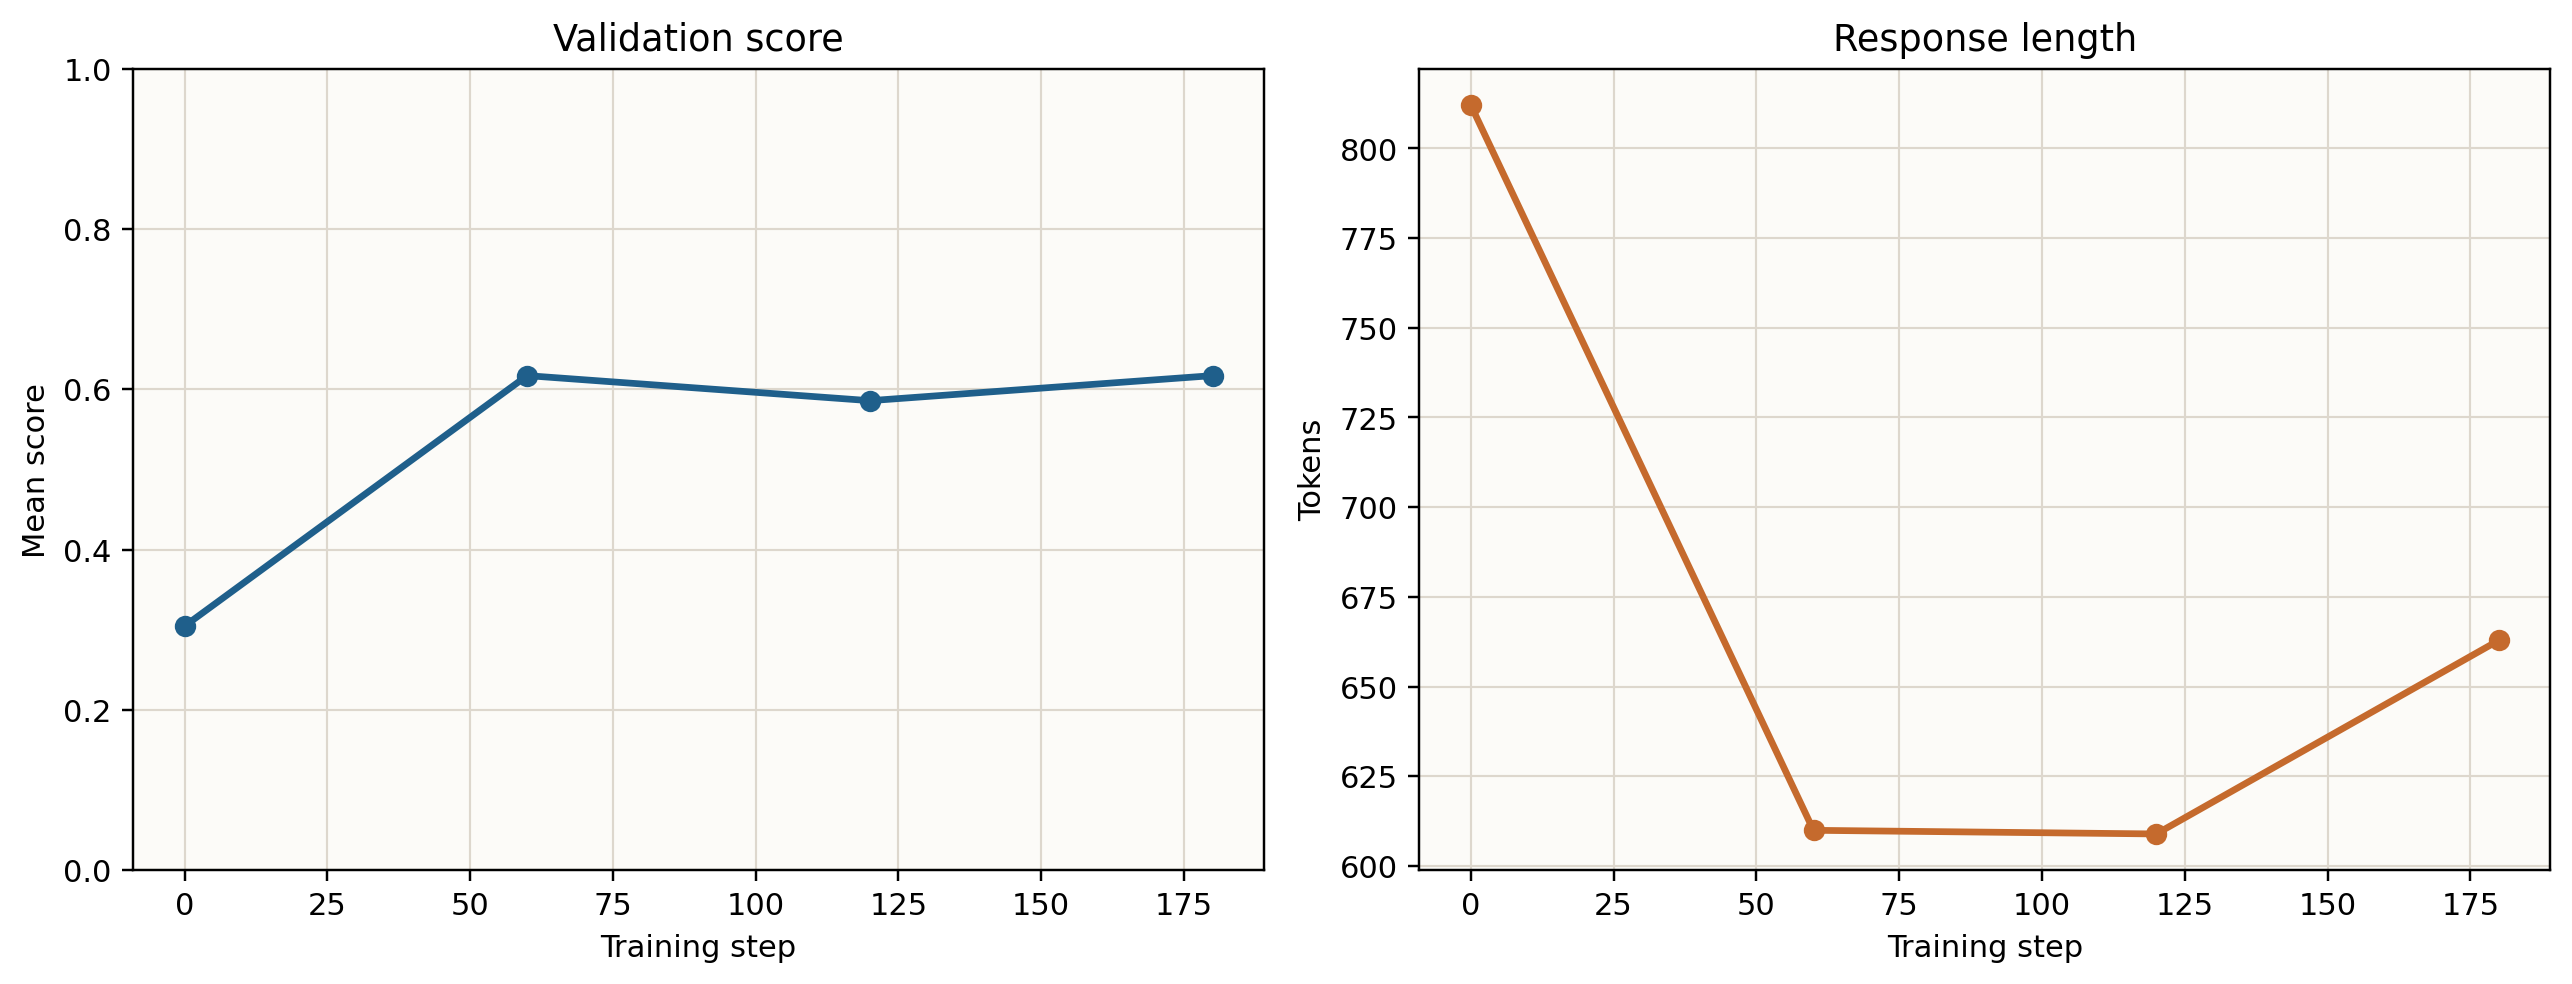
\includegraphics[width=\textwidth]{full-token-score-length.png}
    \caption{Offline full-token audit: validation score and response length across saved checkpoints.}
    \label{fig:en-full-token-score-length}
\end{figure}

\begin{figure}[H]
    \centering
    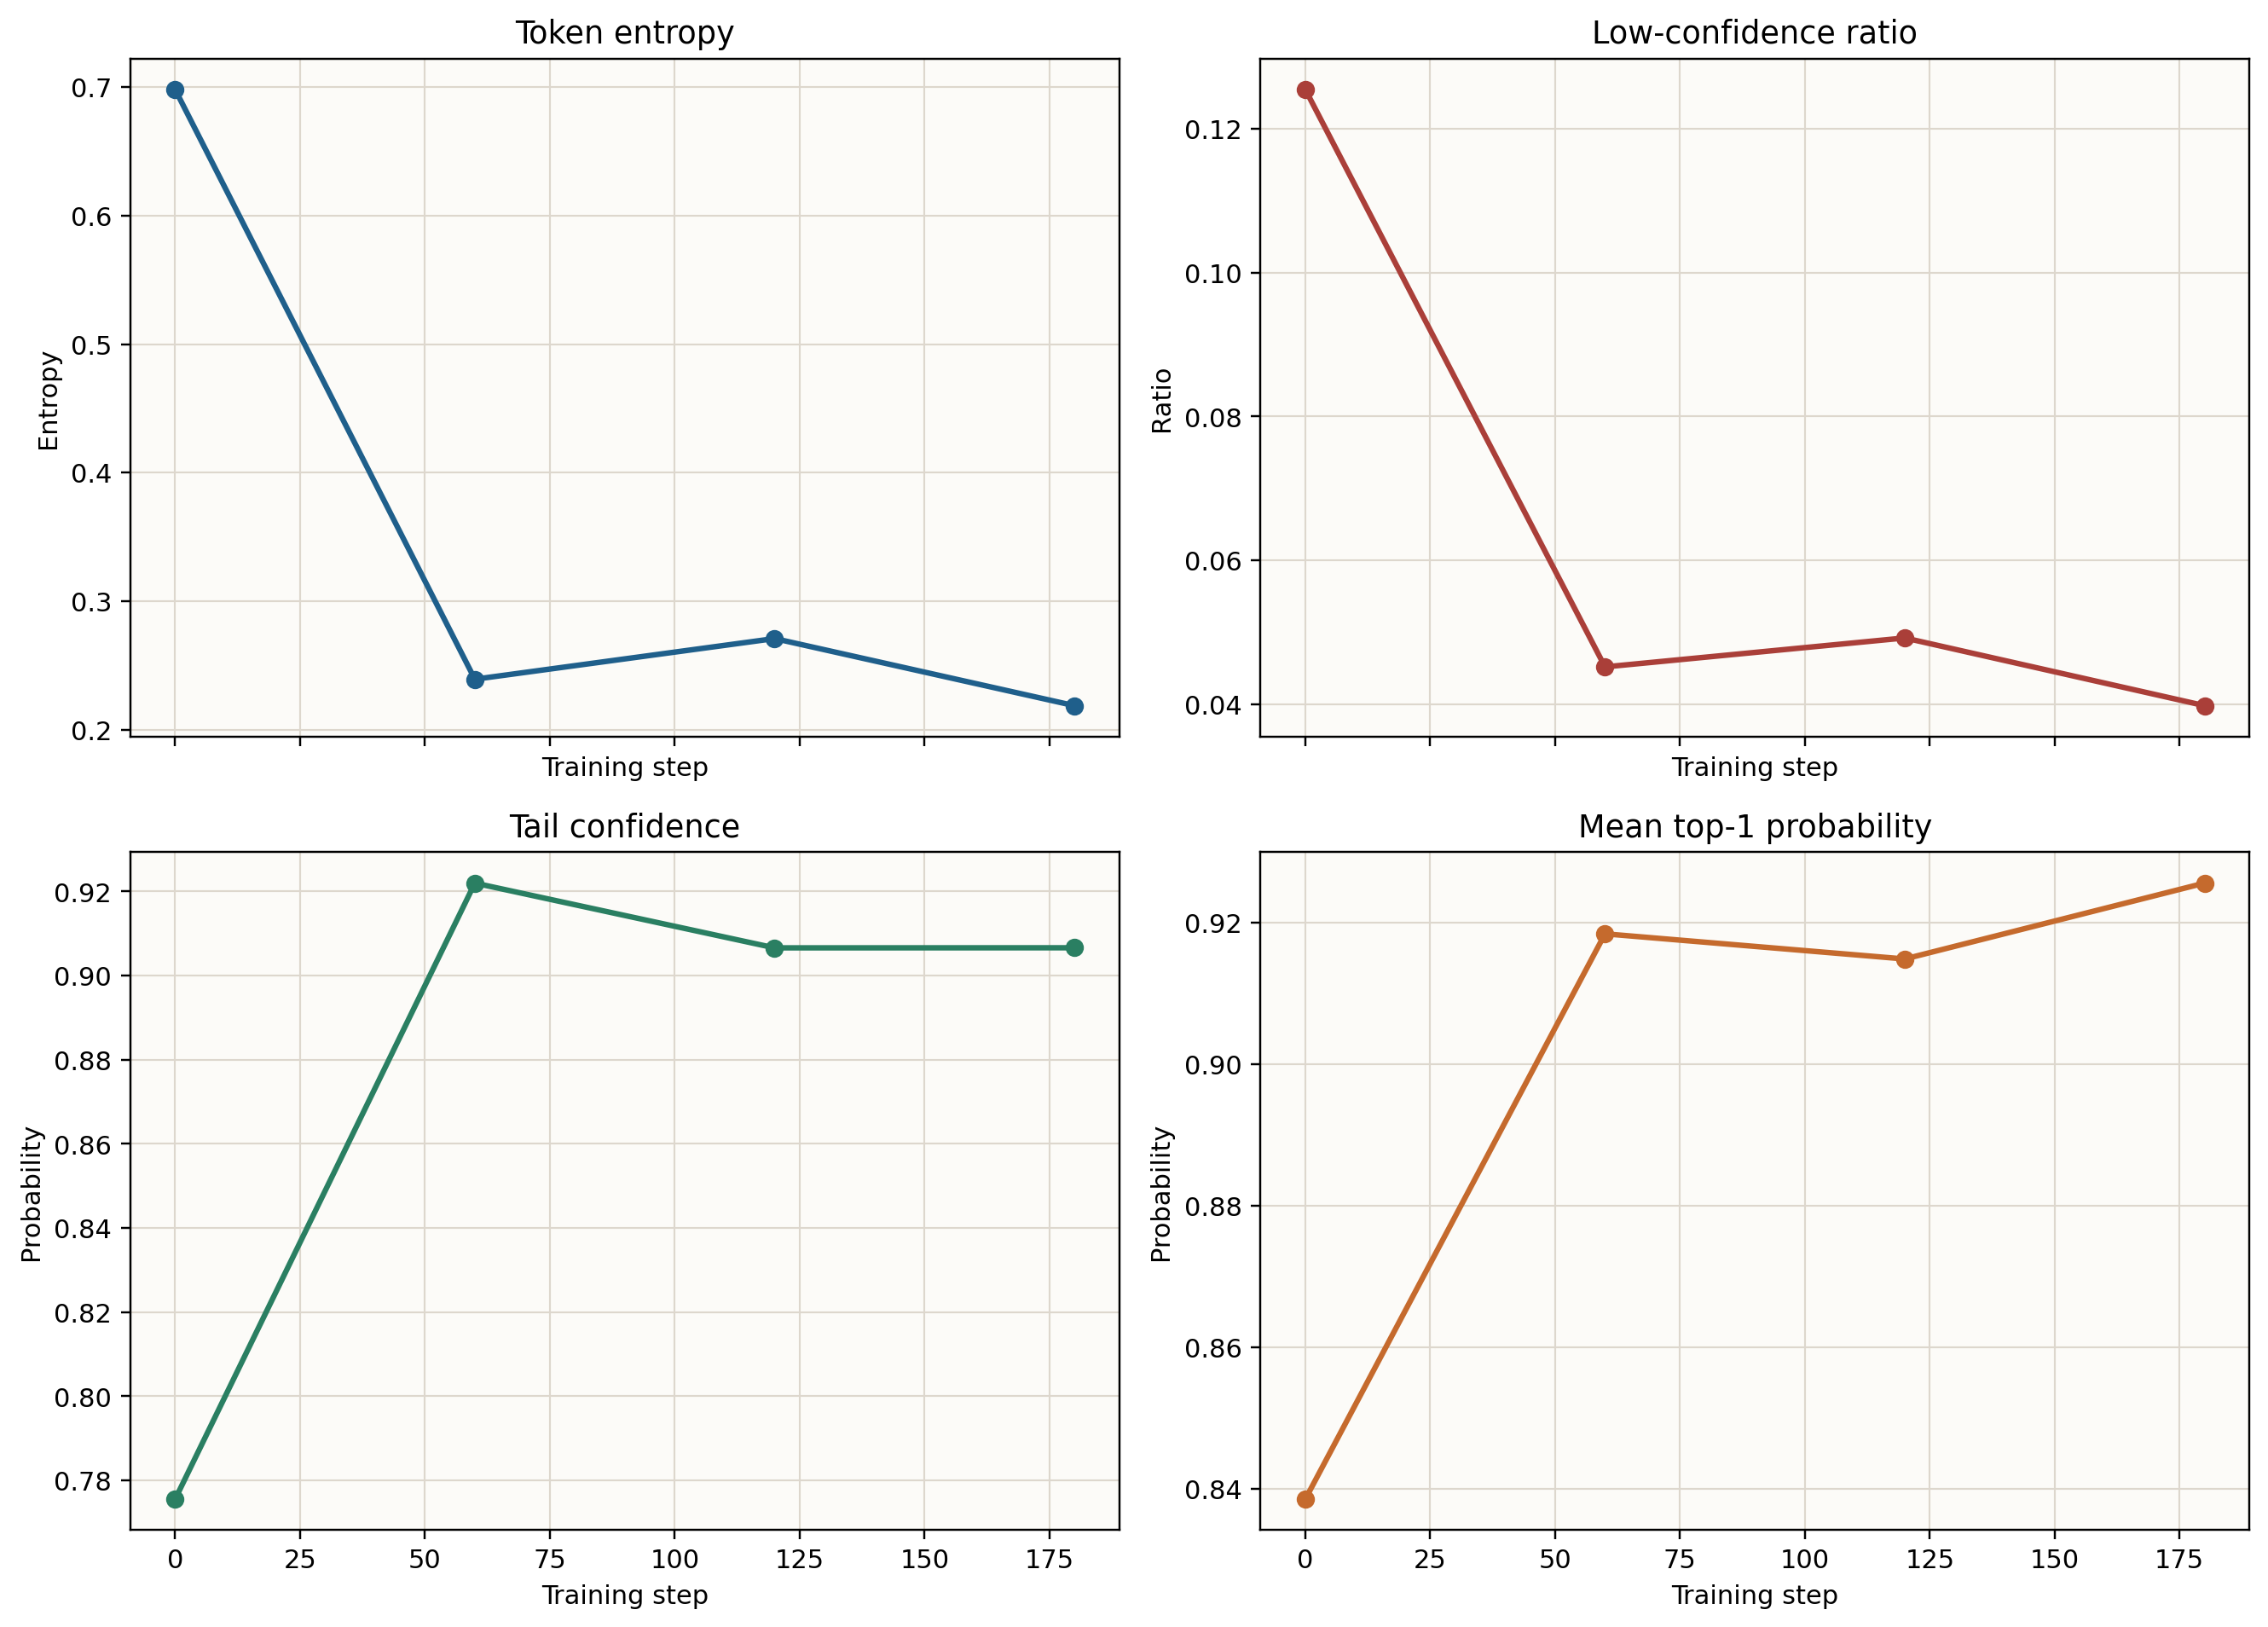
\includegraphics[width=\textwidth]{full-token-confidence-panel.png}
    \caption{Offline full-token audit: token entropy, low-confidence mass, tail confidence, and chosen-token probability across saved checkpoints.}
    \label{fig:en-full-token-confidence-panel}
\end{figure}

\begin{figure}[H]
    \centering
    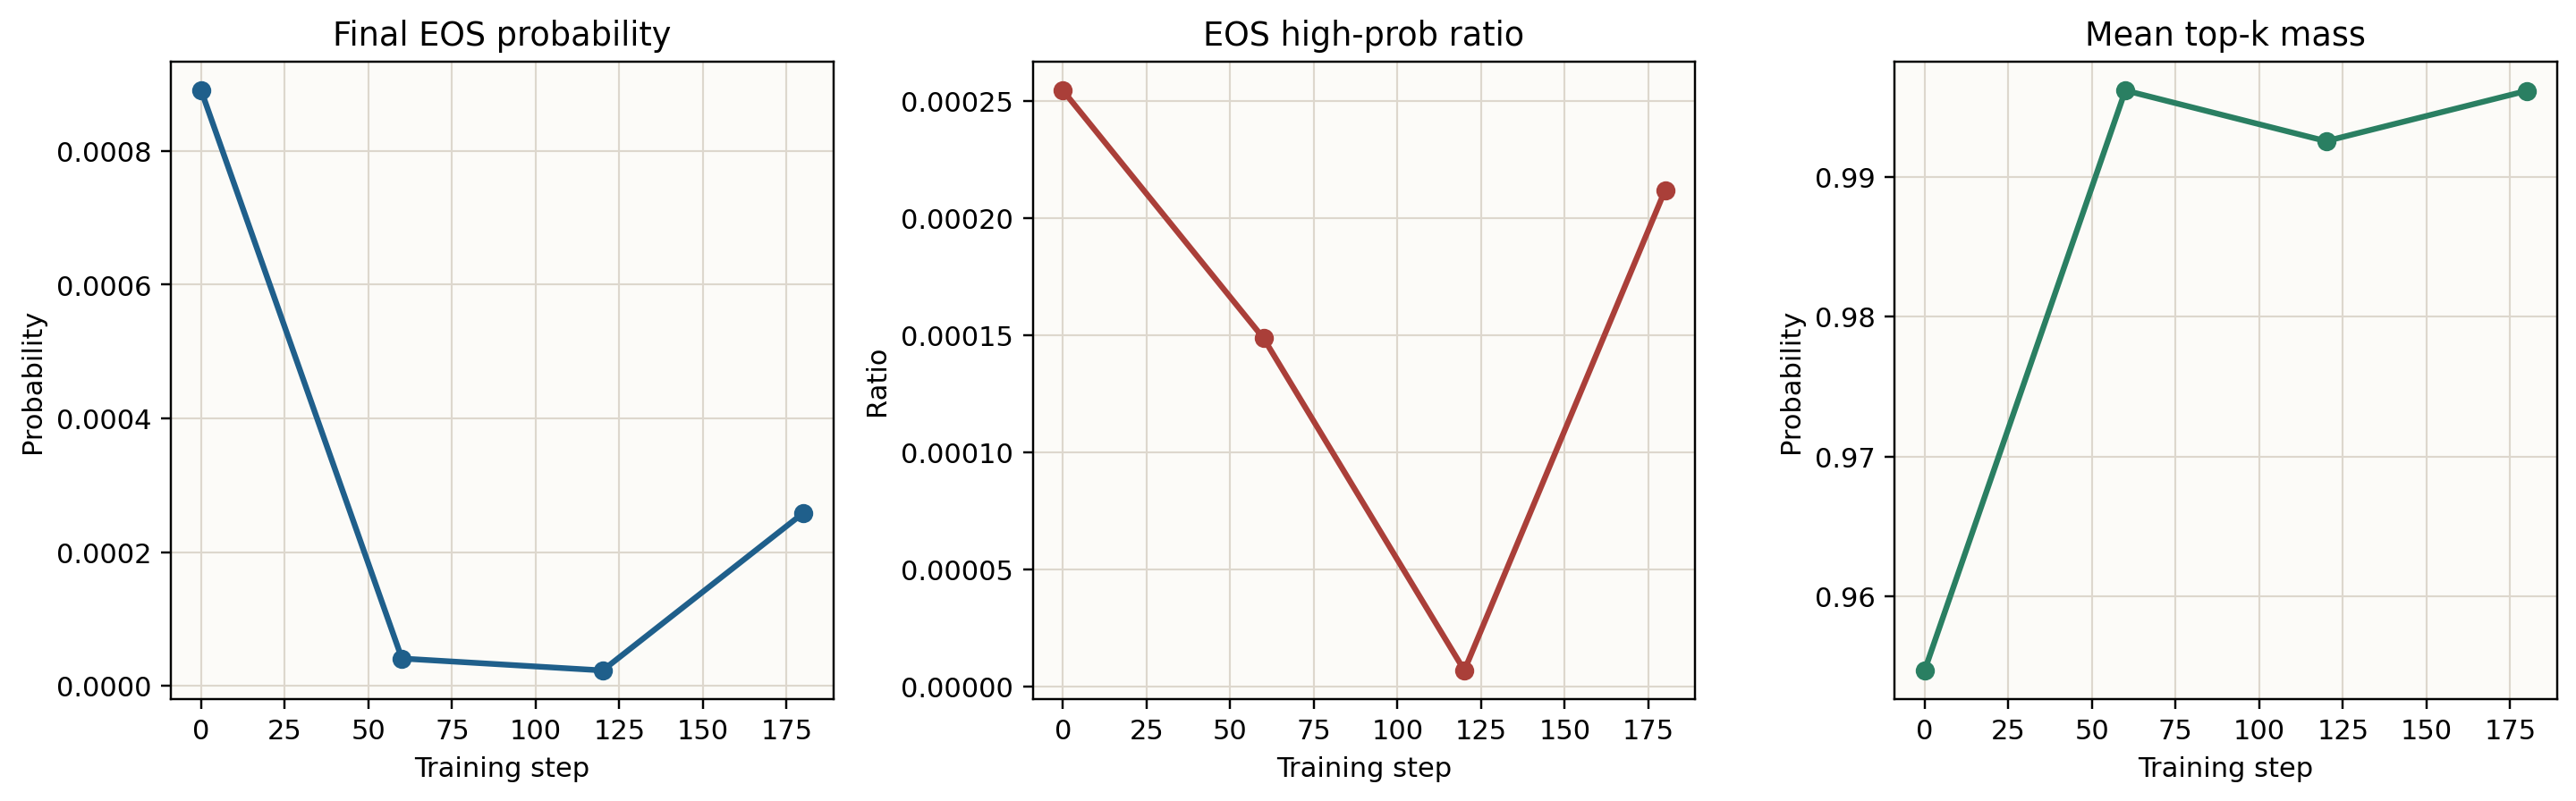
\includegraphics[width=\textwidth]{full-token-eos-topk-panel.png}
    \caption{Offline full-token audit: EOS behavior, top-1 probability, and top-k mass across saved checkpoints.}
    \label{fig:en-full-token-eos-topk-panel}
\end{figure}

\begin{figure}[H]
    \centering
    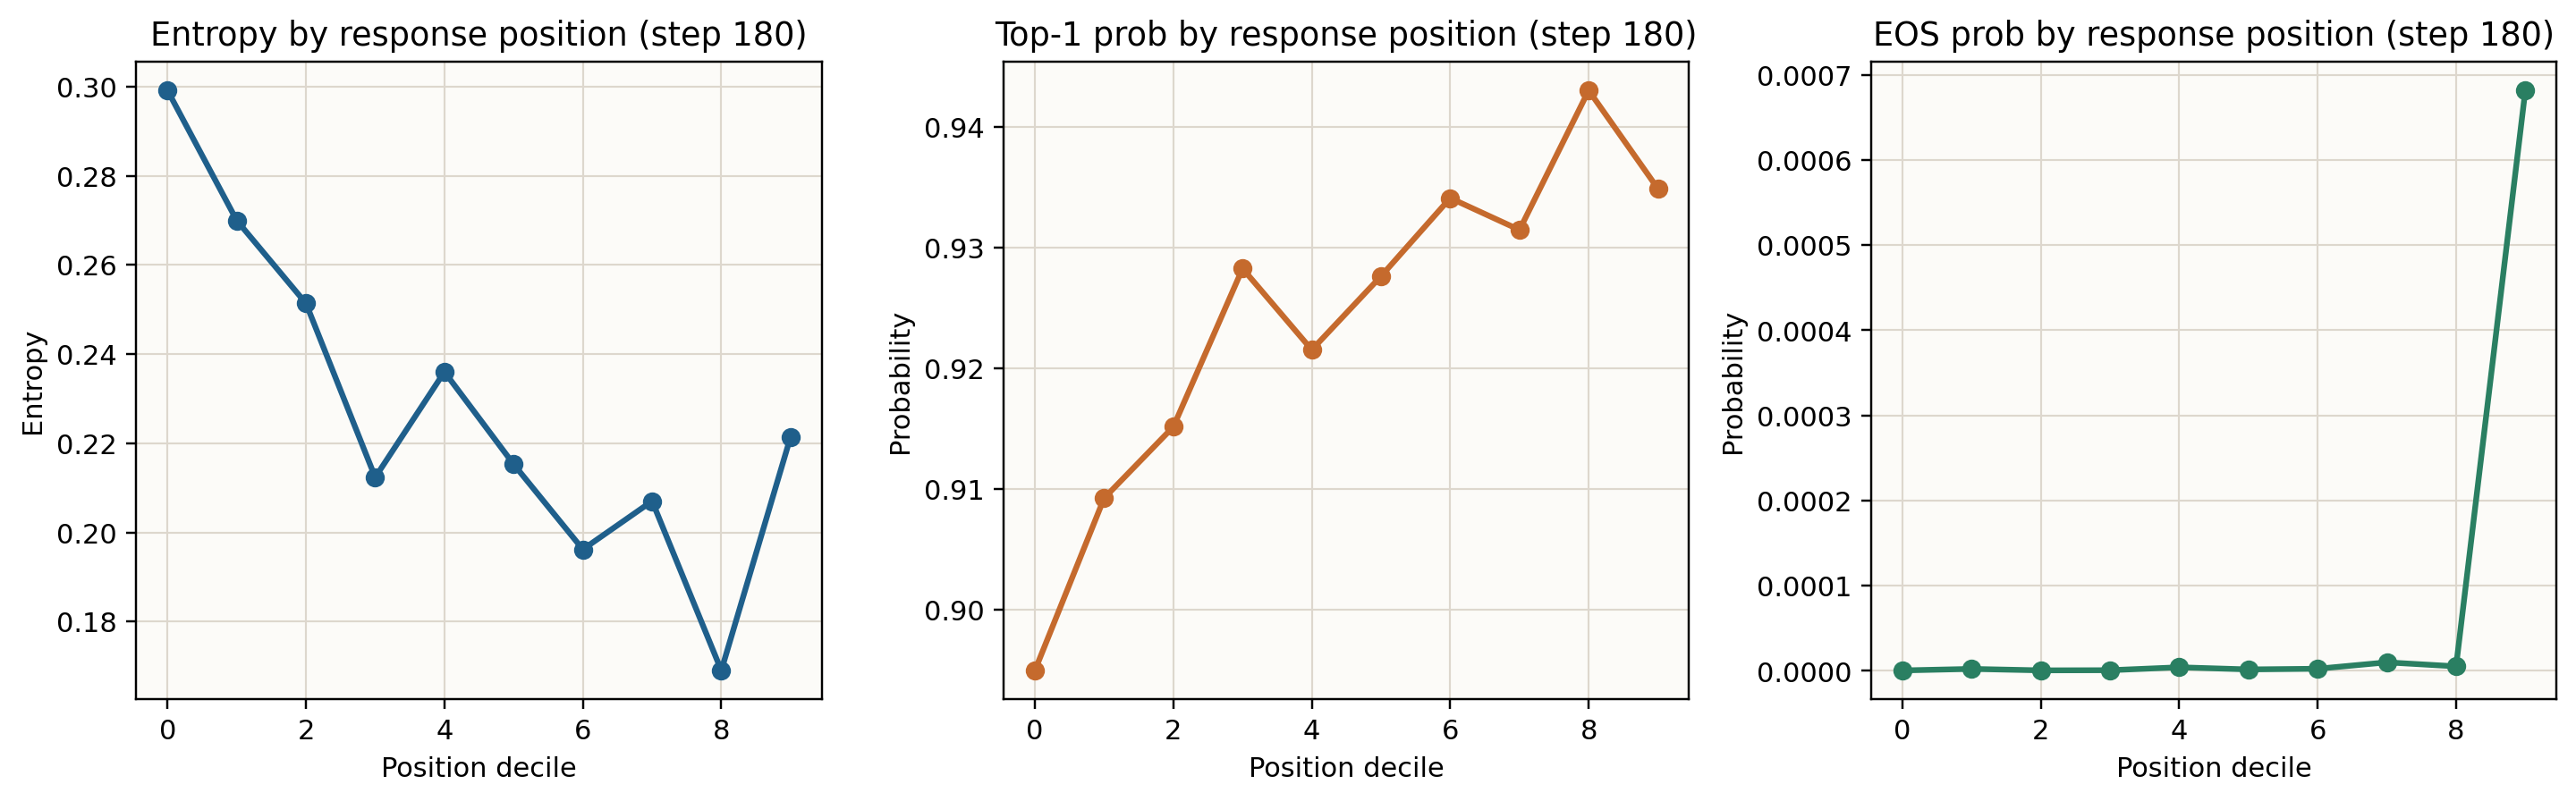
\includegraphics[width=\textwidth]{full-token-position-final.png}
    \caption{Final-checkpoint full-token statistics by relative response position. The x-axis bins generated tokens into response-position deciles.}
    \label{fig:en-full-token-position-final}
\end{figure}

\begin{figure}[H]
    \centering
    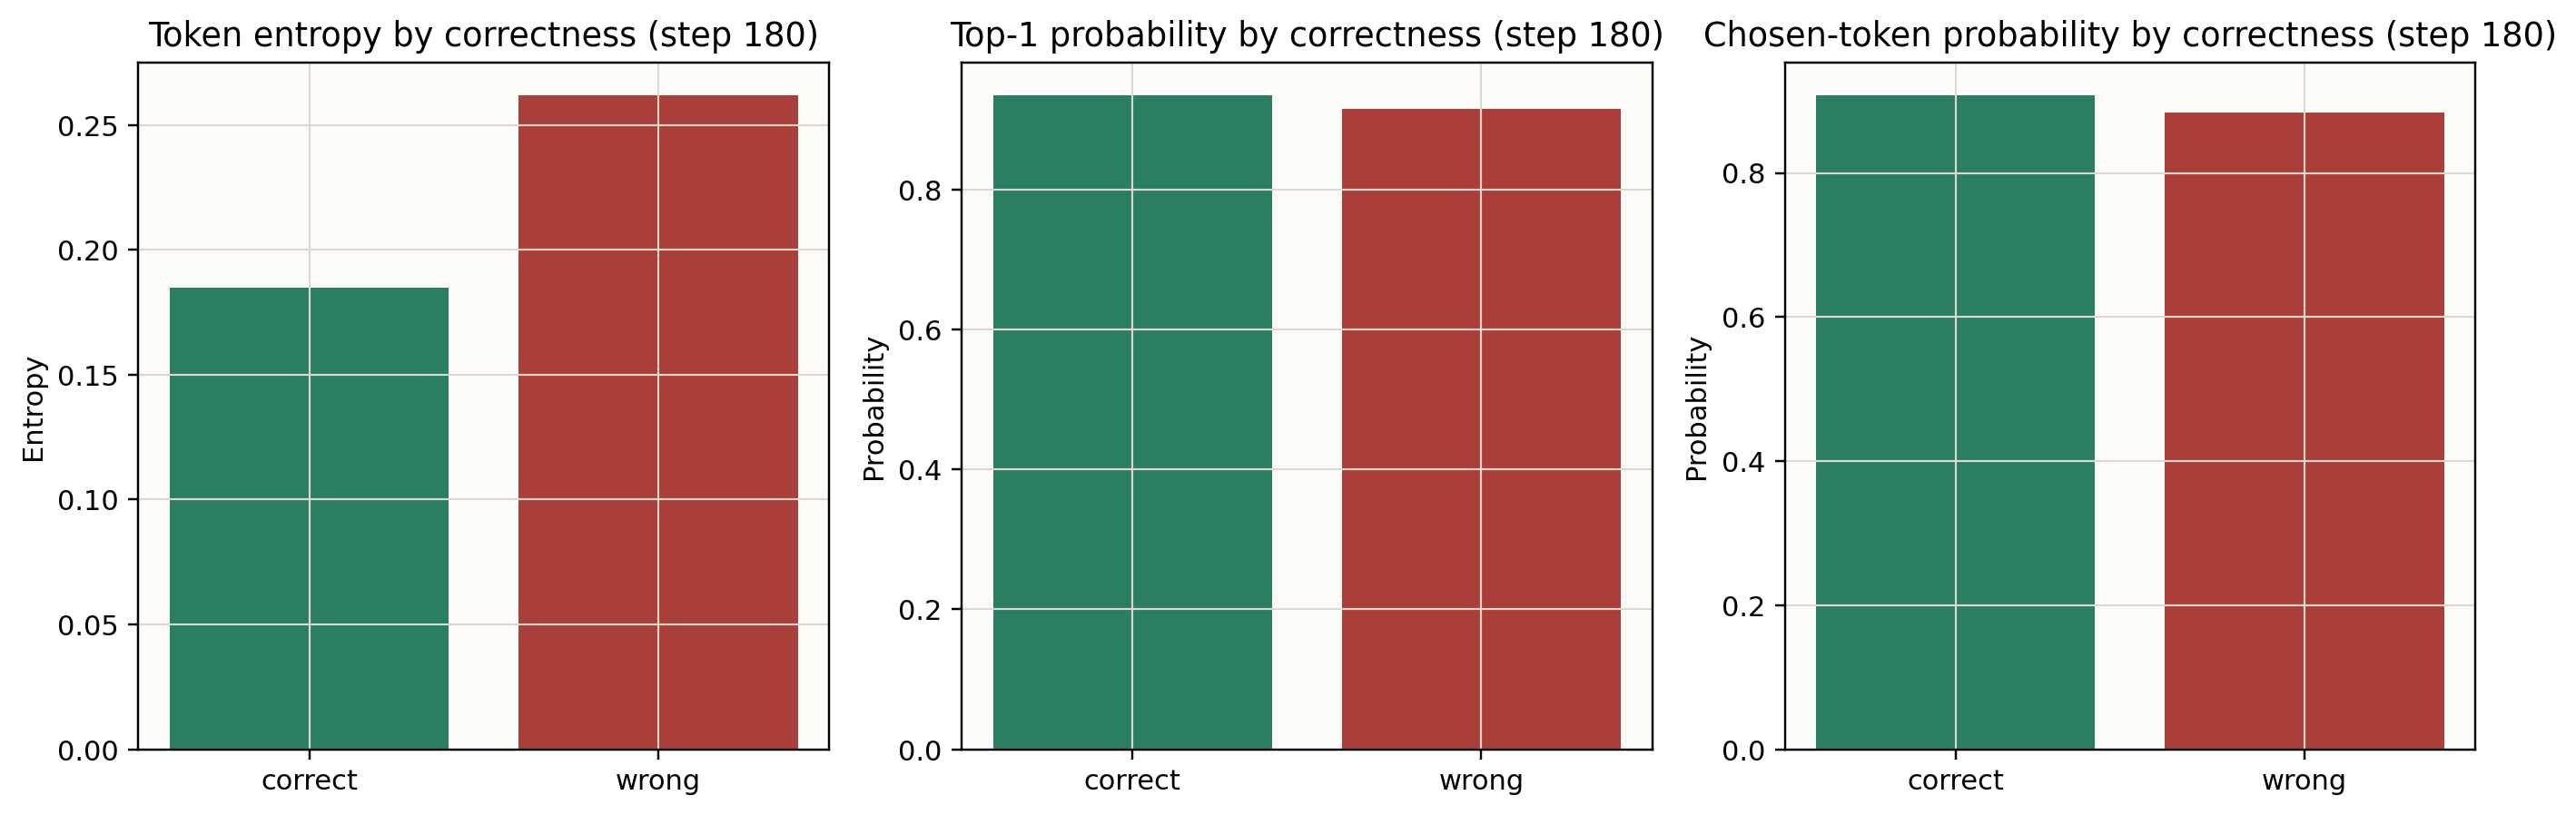
\includegraphics[width=\textwidth]{full-token-correctness-final.png}
    \caption{Final-checkpoint full-token statistics grouped by response correctness.}
    \label{fig:en-full-token-correctness-final}
\end{figure}

The audit strengthens the evidence hierarchy in the paper. The original validation curves show that performance improves; the aggregate token summaries show that the improvement is accompanied by shorter and sharper generations; and this checkpoint audit shows that the same behavior is visible when saved checkpoints are used for fresh full-response inference. Because the audit is based on 32 held-out problems, its numerical values should be read as subset estimates. Its role is mechanism validation: it checks whether the token-level story remains coherent when the analysis is expanded from retained prefixes to complete generated sequences, while also showing why best-checkpoint, final-checkpoint, and token-behavior evidence should be reported together.

}{}

\begin{figure}[H]
    \centering
    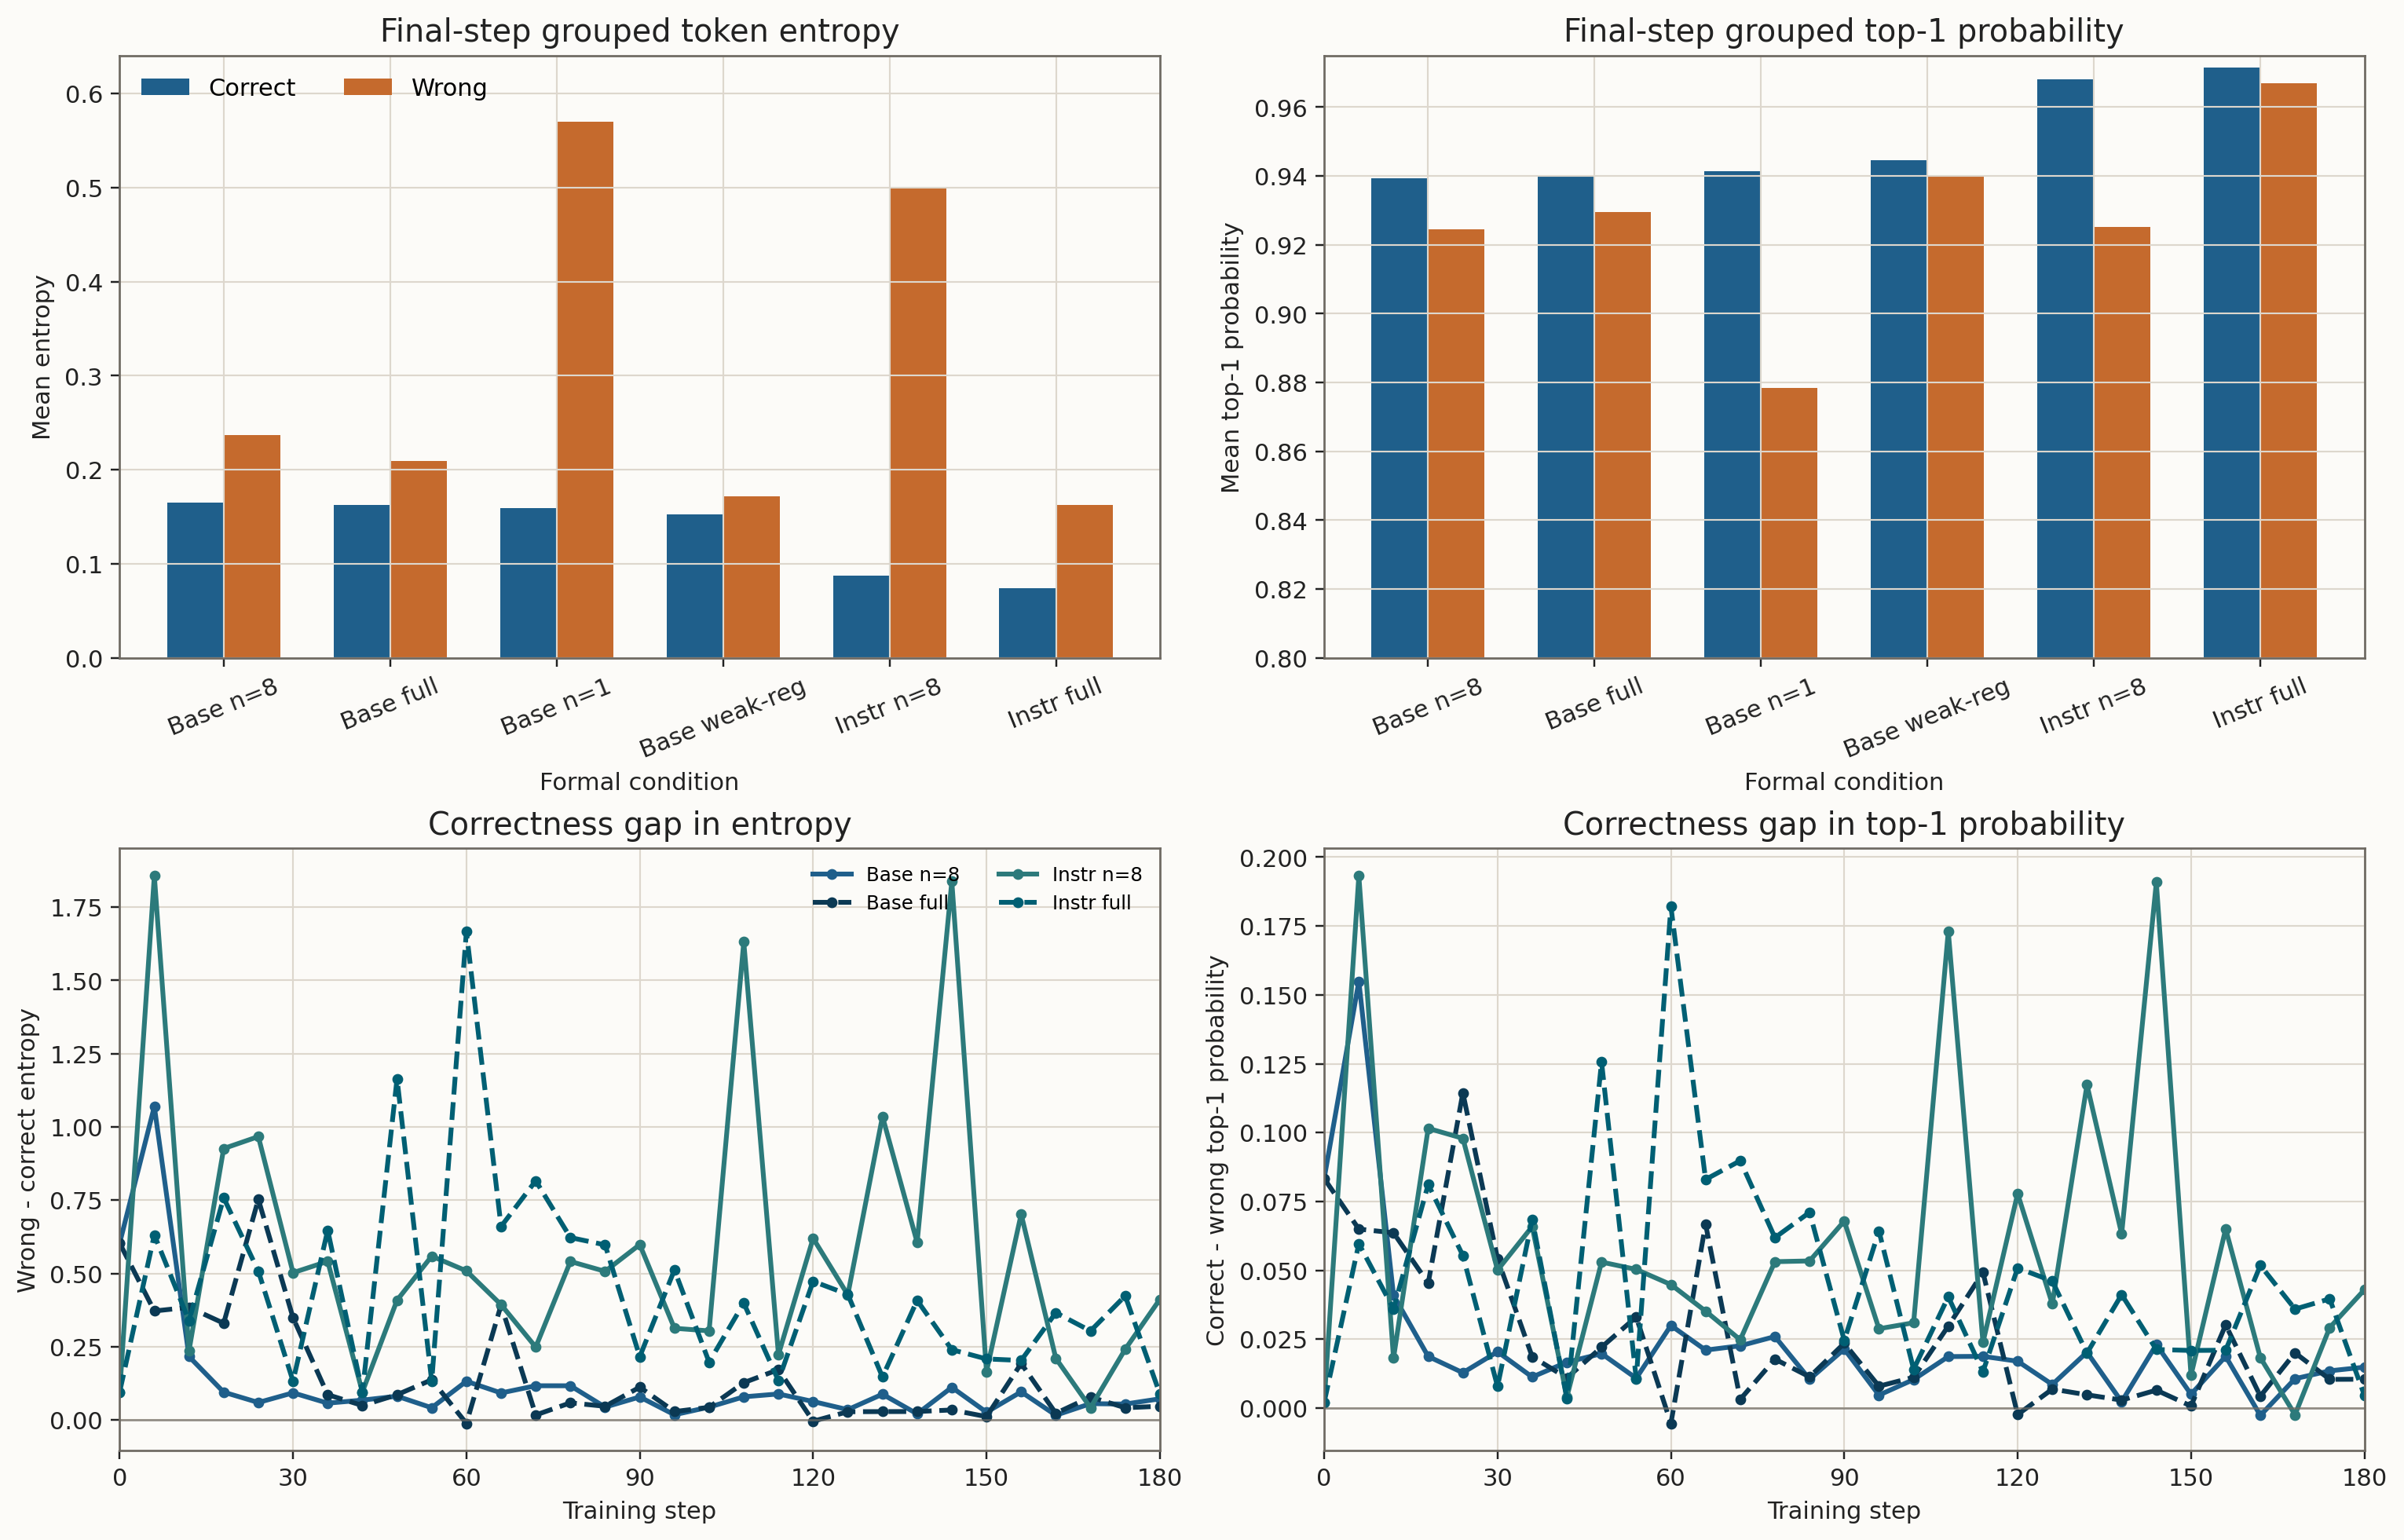
\includegraphics[width=\textwidth]{correct-wrong-support-panel.png}
    \caption{Correctness-conditioned token-distribution statistics. The top row compares final-checkpoint correct and wrong responses across the six non-collapse settings; the bottom row tracks correctness-conditioned gaps over training for the matched one-shot/full-data pairs in the Base and Instruct families.}
    \label{fig:en-correct-wrong-support-panel}
\end{figure}

\begin{table}[H]
    \centering
    \caption{Final-checkpoint correctness-conditioned token summaries}
    \label{tab:en-correct-wrong-final-summary}
    \scriptsize
    \setlength{\tabcolsep}{3pt}
    \begin{tabularx}{\textwidth}{>{\raggedright\arraybackslash}p{0.22\textwidth}ccccc}
        \toprule
        Setting & C/W samples & entropy C/W & top-1 C/W & EOS C/W & tail C/W \\
        \midrule
        Base n=8 & 47/17 & 0.165/0.237 & 0.939/0.925 & 0.002/0.001 & 0.957/0.866 \\
        Base full-data & 51/13 & 0.162/0.209 & 0.940/0.929 & 0.003/0.002 & 0.944/0.885 \\
        Base n=1 & 45/19 & 0.159/0.570 & 0.941/0.878 & 0.003/0.011 & 0.949/0.785 \\
        Base weak-reg. & 51/13 & 0.152/0.172 & 0.945/0.940 & 0.002/0.001 & 0.958/0.889 \\
        Instruct n=8 & 57/7 & 0.087/0.499 & 0.968/0.925 & 0.002/0.002 & 0.973/0.830 \\
        Instruct full-data & 57/7 & 0.074/0.163 & 0.972/0.967 & 0.002/0.002 & 0.978/0.877 \\
        \bottomrule
    \end{tabularx}
\end{table}

Table~\ref{tab:en-correct-wrong-final-summary} gives the numerical counterpart of Figure~\ref{fig:en-correct-wrong-support-panel}. C/W denotes correct and wrong response groups. All six non-collapse settings show the same direction: correct responses have lower token entropy and higher mean top-1 probability than wrong responses. This moves the calibration argument beyond global averages. The model is not only becoming sharper overall; successful responses are more concentrated in the low-entropy and high-confidence region.

\begin{table}[H]
    \centering
    \caption{Correctness-conditioned gaps for matched one-shot/full-data pairs}
    \label{tab:en-correct-wrong-gap-summary}
    \small
    \begin{tabular}{lcccc}
        \toprule
        Setting & step-0 entropy gap & final entropy gap & step-0 top-1 gap & final top-1 gap \\
        \midrule
        Base n=8 & 0.603 & 0.072 & 0.0833 & 0.0149 \\
        Base full-data & 0.603 & 0.047 & 0.0833 & 0.0105 \\
        Instruct n=8 & 0.095 & 0.412 & 0.0021 & 0.0429 \\
        Instruct full-data & 0.095 & 0.089 & 0.0021 & 0.0047 \\
        \bottomrule
    \end{tabular}
\end{table}

Table~\ref{tab:en-correct-wrong-gap-summary} focuses on the matched pairs. The entropy gap is wrong minus correct, and the top-1 gap is correct minus wrong, so positive values indicate that correct responses are lower-entropy and higher-confidence. The Base one-shot and full-data settings share the same initial gap, confirming that their starting points are comparable. By the final checkpoint, both preserve a positive gap, while full-data produces a more compact wrong-response group. The Instruct pair also shares the same initial gap, but \texttt{Instruct full-data} ends with a much smaller entropy gap than \texttt{Instruct n=8}, consistent with a stronger prior and more uniform endpoint behavior.

\section{Group Size, Reward Signal, and Validity Risks}

\subsection{Interpreting the \texttt{n=1} group-size setting}

\texttt{Base n=1} yields a matched-protocol comparison. It improves from 0.3630 to 0.5470, with a best score of 0.5590, which demonstrates that reducing the group size to 1 does not eliminate learning.

At the same time, the matched comparison directly argues against the claim that group size is irrelevant. Under the same \texttt{val\_rollout\_n=8} protocol, \texttt{n=1} is consistently weaker than \texttt{n=8}. The resulting conclusion is that group-relative signal is not necessary for gains to exist, but it appears important for reaching the best and most stable final regime. The remaining caution is that the comparison is still single-seed rather than multi-seed.

\subsection{Random-reward setting}

The random-reward setting addresses a central causal issue: whether the gains are driven by meaningful supervision, or whether a randomized reward signal can produce similar gains. It is particularly informative because it directly tests whether the meaningful-reward improvement depends on the integrity of the reward signal.

\begin{table}[H]
    \centering
    \caption{Endpoint behavior of the random-reward setting}
    \label{tab:en-random-reward-endpoint}
    \begin{tabular}{lc}
        \toprule
        Metric & Value \\
        \midrule
        final score & 0.00025 \\
        final response length & 1192.4 \\
        final tail confidence & 0.0001 \\
        final low-confidence ratio & 1.0000 \\
        final token entropy & 11.5466 \\
        final EOS probability & 0.0009 \\
        final top-1 probability & 0.0021 \\
        \bottomrule
    \end{tabular}
\end{table}

Trained under random wrong rewards, \texttt{Base random-reward} collapses rather than merely failing to improve. It begins at 0.3630 but falls to 0.00025 by the end of training; response length grows from 762.8 to 1192.4, low-confidence mass saturates to 1.0000, token entropy rises to 11.5466, final EOS probability falls to 0.0009, and mean top-1 probability collapses to 0.0021. Table~\ref{tab:en-random-reward-endpoint} summarizes this endpoint regime. This result shows that the meaningful-reward gains are not reproduced when supervision is actively corrupted. It should not be read as a pure no-signal ablation: the setting injects wrong reward information, making it an intentionally severe reward-corruption control.

\section{Training Dynamics and Evidence Synthesis}

\subsection{Phase distribution of gains}

The final score does not reveal when the gains are realized. Figure~\ref{fig:en-phase-gain-breakdown} decomposes the score change of each setting into three coarse phases: \texttt{0$\rightarrow$36}, \texttt{36$\rightarrow$96}, and \texttt{96$\rightarrow$180}. The decomposition is intentionally simple, but it is sufficient to distinguish fast early correction from mid-stage consolidation and late-stage fluctuation.

The pattern is consistent with the paper's main interpretation. In the Base family, most of the improvement arrives in the first two phases, especially in the rapid \texttt{0$\rightarrow$36} stage. This is consistent with a calibration interpretation: the model is first moved out of its unstable initial regime, then consolidated, and only later enters a more variable high-score region. The Instruct family, by contrast, shows little meaningful phase-wise gain, which reinforces the claim that this setting behaves more like local refinement than like structural reorganization.

\begin{figure}[H]
    \centering
    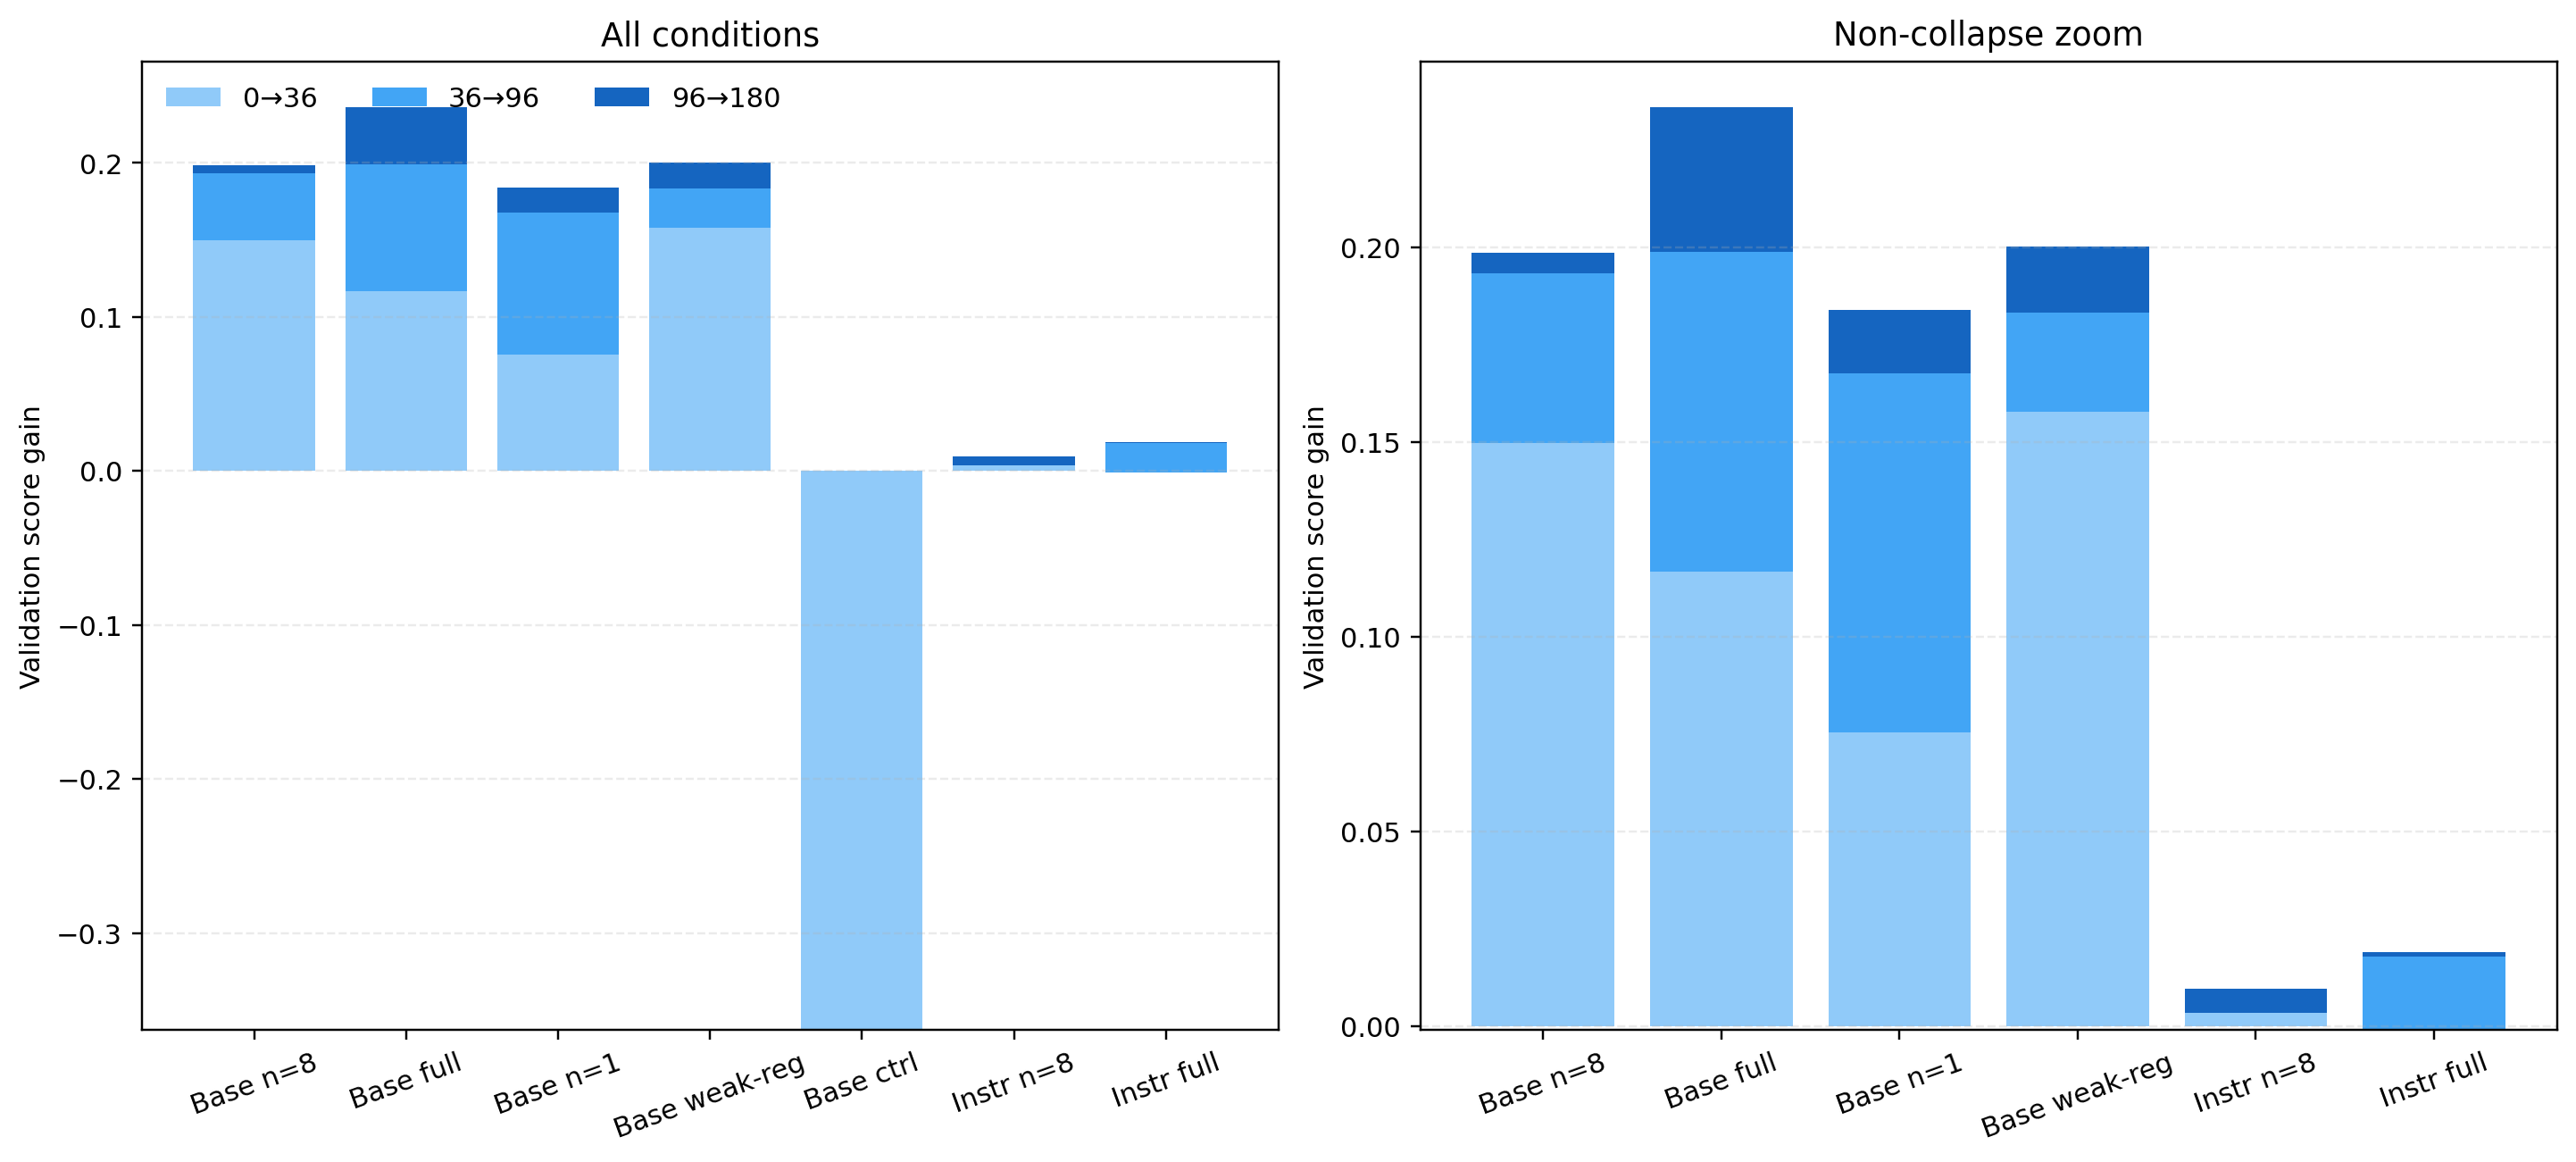
\includegraphics[width=\textwidth]{phase-gain-breakdown.png}
    \caption{Stage-wise decomposition of score gains across the seven main-result settings.}
    \label{fig:en-phase-gain-breakdown}
\end{figure}

\subsection{Separating the best and final checkpoints}

Under a low-data RL regime, the best checkpoint and the last checkpoint are often not the same. Figure~\ref{fig:en-best-final-gap} makes this concrete by showing both the \texttt{best score - final score} gap and the step at which the best checkpoint appears. This consolidates an observation that would otherwise remain scattered across the tables: several settings reach their strongest validation point before the end of training.

This distinction matters for interpretation. The training process looks less like a monotonic climb and more like a transition into a higher but somewhat fluctuating regime. For the Base settings, checkpoint selection and early stopping are not secondary engineering details but part of the optimization behavior. For the Instruct setting, once the model is already strong, the later part of training is more likely to manifest as noise than as a large deterministic gain.

\begin{figure}[H]
    \centering
    
\includegraphics[width=\textwidth]{best-final-gap.png}
    \caption{Comparison between the best and final checkpoints across the seven main-result settings.}
    \label{fig:en-best-final-gap}
\end{figure}

\subsection{Final-behavior ranking as supplementary evidence}

Figure~\ref{fig:en-final-behavior-ranking} ranks the seven main-result settings by several final behavioral metrics: token entropy, low-confidence ratio, top-1 probability, and response length. Compared with reporting these numbers separately, the ranking view makes the global structure easier to see. It shows, for example, that the Base-family meaningful-reward settings can end with similar rewards while still exhibiting noticeably different convergence styles. \texttt{Base full-data} improves length and low-confidence mass further, \texttt{Base weak-reg.} shows stronger contraction, \texttt{Base n=8} is more moderate, \texttt{Base n=1} remains visibly worse than \texttt{n=8} on final entropy and low-confidence mass, and \texttt{Base random-reward} lies far outside the convergence region of the non-collapse settings. In the Instruct family, full-data further reduces entropy and low-confidence mass, although the score gain remains much smaller than in the Base family.

The paper should therefore not rely on reward alone. Several Base-family settings cluster very closely in final score, but the ranking plot shows that their endpoint distributions are not interchangeable. The same is true in a different way for the Instruct family: small reward differences can coexist with visibly different token-entropy structure. Together, these observations strengthen the broader methodological point of the paper: the strongest evidence comes from reading score and behavior together rather than reducing everything to a single summary metric.

\begin{figure}[H]
    \centering
    
\includegraphics[width=\textwidth]{final-behavior-ranking.png}
    \caption{Final-behavior ranking across the seven main-result settings.}
    \label{fig:en-final-behavior-ranking}
\end{figure}

\subsection{Cross-metric coupling}

\subsubsection{Coupling between gains and calibration metrics}

The preceding sections separately discuss score trajectories, behavioral endpoints, and token-level supplementary evidence. A stricter test is whether those observations only point in the same direction, or whether they also co-vary at the condition level. Figure~\ref{fig:en-gain-calibration-coupling} addresses this issue by plotting the score gain of the seven main-result settings against four dynamic change magnitudes: the reduction in training-time actor entropy, the reduction in validation token entropy, the reduction in low-confidence token ratio, and the reduction in validation response length. The actor-entropy panel follows training-log availability, whereas the validation-token panels include the full-data runs.

Figure~\ref{fig:en-gain-calibration-coupling} turns the calibration interpretation into a tighter empirical pattern. The Base-family settings are not only the settings with larger score gains; they are also the settings with larger entropy contraction, larger removal of low-confidence mass, and larger shortening of outputs. The full-data runs extend this pattern by showing that a larger training budget moves the endpoint upward while preserving the same broad relationship between reward gain and distributional stabilization. This coupling is more informative than listing endpoint numbers separately, because it shows that the gain and the stabilization process appear together in the same settings.

\begin{figure}[H]
    \centering
    
\includegraphics[width=\textwidth]{gain-calibration-coupling.png}
    \caption{Coupling between validation score gain and four key dynamic changes across the seven main-result settings. The training-time actor-entropy panel follows log-field availability.}
    \label{fig:en-gain-calibration-coupling}
\end{figure}

\subsubsection{Joint frontier of final performance and stability}

It is also useful to ask whether the settings with better final reward are the same settings that end in more stable output distributions. Figure~\ref{fig:en-endpoint-frontier-panel} places final validation score in a shared coordinate system with two endpoint stability metrics: final token entropy and final low-confidence ratio. With all seven settings included, this frontier-style view also shows where the full-data runs sit relative to their one-shot counterparts.

Within the Base family, the trend is fairly clear: the higher-scoring settings also tend to have lower entropy and lower low-confidence mass. \texttt{Base n=1} remains visibly behind \texttt{Base n=8} on both axes, so its weakness is not confined to a single reward curve; it is reflected in the endpoint distribution itself. The Instruct family occupies a different region: the final scores are higher, but the internal spread is small, which is consistent with a model that already starts in a relatively stable regime.

\begin{figure}[H]
    \centering
    
\includegraphics[width=\textwidth]{endpoint-frontier-panel.png}
    \caption{Joint frontier view of final score and final stability metrics.}
    \label{fig:en-endpoint-frontier-panel}
\end{figure}

\subsubsection{Role of the cross-metric figures}

Together with the preceding sections, these figures strengthen the overall evidential structure. The first layer of evidence is the score improvement itself and the distinction between best and final checkpoints. The second layer is the dynamic change in behavior: length, entropy, top-1 probability, EOS behavior, and low-confidence mass. The third layer is the cross-metric coupling view, which puts those quantities back at the condition level and shows that they move together. This section therefore answers the timing-and-synthesis question: the gain appears early, enters a fluctuating high-score regime, and remains coupled with distributional stabilization across settings.

\section{Discussion}

\subsection{Main supporting evidence}

The strongest part of the evidence is the coherence of the Base-model pattern. Score rises sharply. Response length drops. Tail confidence rises. Low-confidence tokens become rarer. Entropy falls. EOS behavior becomes sharper. The token-level fixed-prompt traces independently show more stable early-token organization, the offline checkpoint audit extends that view to complete generated responses on a held-out subset, and the matched full-data comparisons point in the same direction. Read together, these observations make behavioral calibration the best-supported explanation under the current scope.

\subsection{Remaining limitations}

Four issues remain unresolved. First, the group-size result needs replication across multiple seeds. Second, the random-reward setting has not yet been matched by an Instruct-family counterpart. Third, the current diagnostics support a calibration account, but they do not fully separate calibration from knowledge acquisition across problem domains or difficulty levels. A stronger follow-up would stratify held-out problems by difficulty or topic and test whether gains are uniform, as expected under broad calibration, or concentrated in specific knowledge regions. Fourth, the offline checkpoint audit reduces the earlier 96-token-prefix limitation, but it is still a subset audit and still covers only the checkpoints that were saved for this run; training-time \texttt{actor entropy}, fixed-prompt traces, and full-token offline inference therefore remain complementary rather than perfectly symmetric evidence sources.

\subsection{Practical implications}

The practical implication is clear: under severe data constraints, 1-shot GRPO can still be worthwhile for improving a weaker math reasoning model. The gains are substantive, and they appear to come from making the model more decisive, shorter, and better calibrated. For a model with a strong instruction-tuned prior, expectations should be more modest. In that regime, RL is closer to local refinement than to a large performance transition.

\section{Conclusion}

This paper characterizes the effect of 1-shot GRPO on mathematical reasoning using seven main-result settings, seven-setting aggregate behavioral diagnostics, narrower token-trace evidence, a saved-checkpoint full-token audit, and matched one-shot/full-data contrasts. Across these sources, the overall picture is consistent. The Base model benefits substantially, the Instruct model changes only slightly, and the successful Base settings exhibit a coordinated transition toward shorter, lower-entropy, higher-confidence, and more decisive outputs. The matched full-data comparisons further clarify that 1-shot training captures a meaningful part of the attainable gain but does not close the gap to a larger data budget under the same schedule.

Within that evidence framework, three conclusions are the most defensible. First, 1-shot GRPO is effective for the Base math model under the present low-data regime. Second, the gain is better explained as rapid calibration than as broad mathematical knowledge acquisition, while a difficulty- or topic-stratified evaluation would be needed to fully separate those mechanisms. Third, both group-relative signal and reward integrity matter for the final regime: reducing the training group size from 8 to 1 weakens but does not remove the gain, whereas corrupting the reward signal causes the model to collapse in both score and behavioral stability. The remaining caveats are equally clear. The \texttt{n=1} versus \texttt{n=8} comparison is still single-seed rather than multi-seed, and the random-reward setting has not yet been matched by an Instruct-family counterpart. Within those limits, the current evidence supports interpreting 1-shot GRPO primarily as a low-data stabilization and calibration mechanism for Base mathematical reasoning.

\clearpage
\appendix

\section{Legacy Full-Data and Format-Constrained References}

The main body includes the matched full-data runs as part of the primary comparison. The appendix section below preserves a legacy set of full-data and format-constrained reference results for historical comparison and supplementary context. They are therefore useful as appendix-level background rather than as primary evidence for the main claims.

\begin{table}[H]
    \centering
    \caption{Summary of representative full-data and format-constrained reference results}
    \label{tab:en-full-data-reference-runs}
    \small
    \begin{tabular}{lcccc}
        \toprule
        Model family & Setting & initial & final & best \\
        \midrule
        Base & 1-shot & 0.3630 & 0.5753 & 0.5803 \\
        Base & full & 0.3630 & 0.6053 & 0.6135 \\
        Base & format-constrained reference & 0.3630 & 0.4490 & 0.4785 \\
        Base & 1-shot entropy reference & 0.3630 & 0.5698 & 0.5835 \\
        Instruct & 1-shot & 0.6860 & 0.6928 & 0.6985 \\
        Instruct & full & 0.6860 & 0.7070 & 0.7070 \\
        Instruct & 1-shot reference & 0.6860 & 0.6893 & 0.7005 \\
        Instruct & full reference & 0.6795 & 0.7118 & 0.7118 \\
        \bottomrule
    \end{tabular}
\end{table}

The table serves a narrow but useful purpose. It shows that the main paper narrative is not confined to the main result table alone: the Base family benefits more strongly in absolute score, \texttt{full} training tends to outperform \texttt{1-shot}, and a more heavily format-constrained reference remains substantially weaker. The corresponding visualization is already shown in Figure~\ref{fig:en-full-data-reference-main}; the appendix therefore avoids repeating the same figures and uses this section only as a compact numerical reference. These results should be used as supplementary reference evidence rather than as part of the matched-protocol primary comparison.

\section{Metric Reading Guide}

The main text deliberately reads score and behavior together rather than treating any single auxiliary diagnostic as decisive. That choice is especially important under a low-data RL regime, where the same scalar outcome can be reached through very different generation patterns. Table~\ref{tab:en-metric-reading-guide} therefore records how each diagnostic is interpreted in this paper and where its limits remain. The appendix-level guide is useful because several later figures compare settings in multiple metric spaces at once.

\begin{table}[H]
    \centering
    \caption{How to read the behavioral metrics used in the paper}
    \label{tab:en-metric-reading-guide}
    \scriptsize
    \setlength{\tabcolsep}{4pt}
    \renewcommand{\arraystretch}{1.18}
    \begin{tabular}{>{\raggedright\arraybackslash}p{2.5cm}>{\raggedright\arraybackslash}p{2.2cm}>{\raggedright\arraybackslash}p{4.2cm}>{\raggedright\arraybackslash}p{4.4cm}}
        \toprule
        Metric & Typical favorable movement & What it reflects & Main caveat \\
        \midrule
        Validation score & higher & Task-level correctness on held-out mathematical problems & Score alone does not reveal whether the model improved by better calibration, shorter search, or some other behavioral route. \\
        Response length & lower & Less wandering and earlier commitment once the answer path is stabilized & Shorter outputs are only favorable when score is preserved or improved; otherwise they can reflect premature stopping. \\
        Answer-tail confidence & higher & More confidence around the answer-bearing tail of the response & Tail confidence is informative only when paired with correctness, because confident wrong answers remain possible. \\
        Low-confidence token ratio & lower & Less probability mass spent on highly uncertain token decisions & The absolute level depends on prompt difficulty, so cross-setting comparisons are more informative than any universal threshold. \\
        Mean token entropy & lower & Sharper next-token distributions and less diffuse local uncertainty & Lower entropy can also appear under pathological collapse, which is why the random-reward case must be read jointly with score and EOS behavior. \\
        Final EOS probability & higher & Clearer stopping behavior near the end of generation & A sharp EOS signal is only useful when it accompanies correct or improved answers rather than truncated failure. \\
        Mean top-1 probability & higher & Stronger concentration on the most likely next token & High top-1 mass by itself does not distinguish correct confidence from confidently wrong behavior. \\
        \bottomrule
    \end{tabular}
\end{table}

Three reading rules follow from Table~\ref{tab:en-metric-reading-guide}. First, no single diagnostic is treated as a stand-alone success criterion apart from held-out score. Second, the most persuasive evidence comes from coordinated movement across metrics, such as shorter responses together with lower entropy and fewer low-confidence tokens. Third, the reward-corruption setting is informative precisely because it separates benign entropy contraction from pathological collapse: in that setting, entropy is not merely low or high in isolation, but coupled to vanishing score, saturated low-confidence mass, and near-zero EOS/top-1 probability.

\section{End-State Behavioral Summary for the Five Key Settings}

The main body emphasizes trajectories because the path into the final regime is central to the paper's interpretation. For quick appendix-level reference, however, it is also useful to collect the endpoint behavior of the five diagnostic settings in one place. Table~\ref{tab:en-appendix-endpoints} plays that role and can be read as the numerical companion to the main trajectory figures.

\begin{table}[H]
    \centering
    \caption{Final behavioral endpoints across the five diagnostic settings}
    \label{tab:en-appendix-endpoints}
    \scriptsize
    \setlength{\tabcolsep}{3.2pt}
    \renewcommand{\arraystretch}{1.15}
    \begin{threeparttable}
    \begin{tabular}{lccccccc}
        \toprule
        Setting & score & length & tail conf. & low-conf. & entropy & EOS & top-1 \\
        \midrule
        Base n=8 & 0.5733 & 603.1 & 0.9331 & 0.0325 & 0.1839 & 0.9880 & 0.9354 \\
        Base n=1 & 0.5470 & 580.4 & 0.9003 & 0.0488 & 0.2811 & 0.9215 & 0.9227 \\
        Base weak-reg. & 0.5747 & 578.6 & 0.9437 & 0.0294 & 0.1563 & 0.9738 & 0.9437 \\
        Base random-reward & 0.0003 & 1192.4 & 0.0001 & 1.0000 & 11.5466 & 0.0009 & 0.0021 \\
        Instruct n=8 & 0.6873 & 470.3 & 0.9571 & 0.0187 & 0.1322 & 0.9926 & 0.9634 \\
        \bottomrule
    \end{tabular}
    \begin{tablenotes}[flushleft]
        \footnotesize
        \item Note: Length is measured in tokens. The behavioral metrics are validation-time endpoints and should be interpreted jointly with score rather than as stand-alone optimization targets.
    \end{tablenotes}
    \end{threeparttable}
\end{table}

The table compresses the paper's central comparison into a reader-friendly endpoint view. The successful Base settings cluster in a relatively narrow region of low entropy, low low-confidence mass, and high EOS/top-1 probability, while \texttt{Base random-reward} lies far outside that region. \texttt{Instruct n=8} finishes with the strongest endpoint profile overall, but its gain from initialization remains small. That contrast is exactly why the paper treats starting prior and gain scale as separate interpretive dimensions.

\clearpage
\section{Matched \texttt{n=1} versus \texttt{n=8}: A Compact Side-by-Side View}

The main text already argues that the \texttt{n=1} group-size setting remains useful but does not fully match \texttt{n=8}. Figure~\ref{fig:en-appendix-aligned-n1n8} makes that comparison easier to inspect by placing the matched score curve beside five core behavioral trajectories. It is included in the appendix because the point is comparative rather than foundational: the paper's main claim does not depend on this compact view, but the view helps the reader inspect the shape of the difference directly.

\begin{figure}[H]
    \centering
    
\includegraphics[width=\textwidth,height=0.82\textheight,keepaspectratio]{aligned-n1-vs-n8-panel.png}
    \caption{Matched comparison between \texttt{Base n=8} and \texttt{Base n=1} across score, response length, token entropy, low-confidence ratio, top-1 probability, and actor entropy.}
    \label{fig:en-appendix-aligned-n1n8}
\end{figure}

The compact panel supports two observations that are easy to miss when each metric is read separately. First, \texttt{n=1} is not merely lower at the end; it also contracts more slowly in entropy and low-confidence mass during the early and middle phases of training. Second, the gap is not uniform across diagnostics. Final response length is not dramatically worse for \texttt{n=1}, but token entropy, low-confidence ratio, and top-1 probability remain consistently weaker, which fits the interpretation that the group-relative signal mainly strengthens distributional stabilization rather than simply shortening answers.

\clearpage
\section{Supplementary Comparison Among the Non-Collapse Settings}

The non-collapse settings are easy to summarize too coarsely if one only says that they all converge to a ``stable'' region. Figure~\ref{fig:en-appendix-main-settings-panel} expands that point by comparing the four non-collapse settings on four endpoint-sensitive metrics: token entropy, low-confidence ratio, final EOS probability, and top-1 probability. Unlike the main body's broader trajectory coverage, this panel is meant as a compact appendix-level synthesis for readers who want to inspect how similar or dissimilar the successful regimes really are.

\begin{figure}[H]
    \centering
    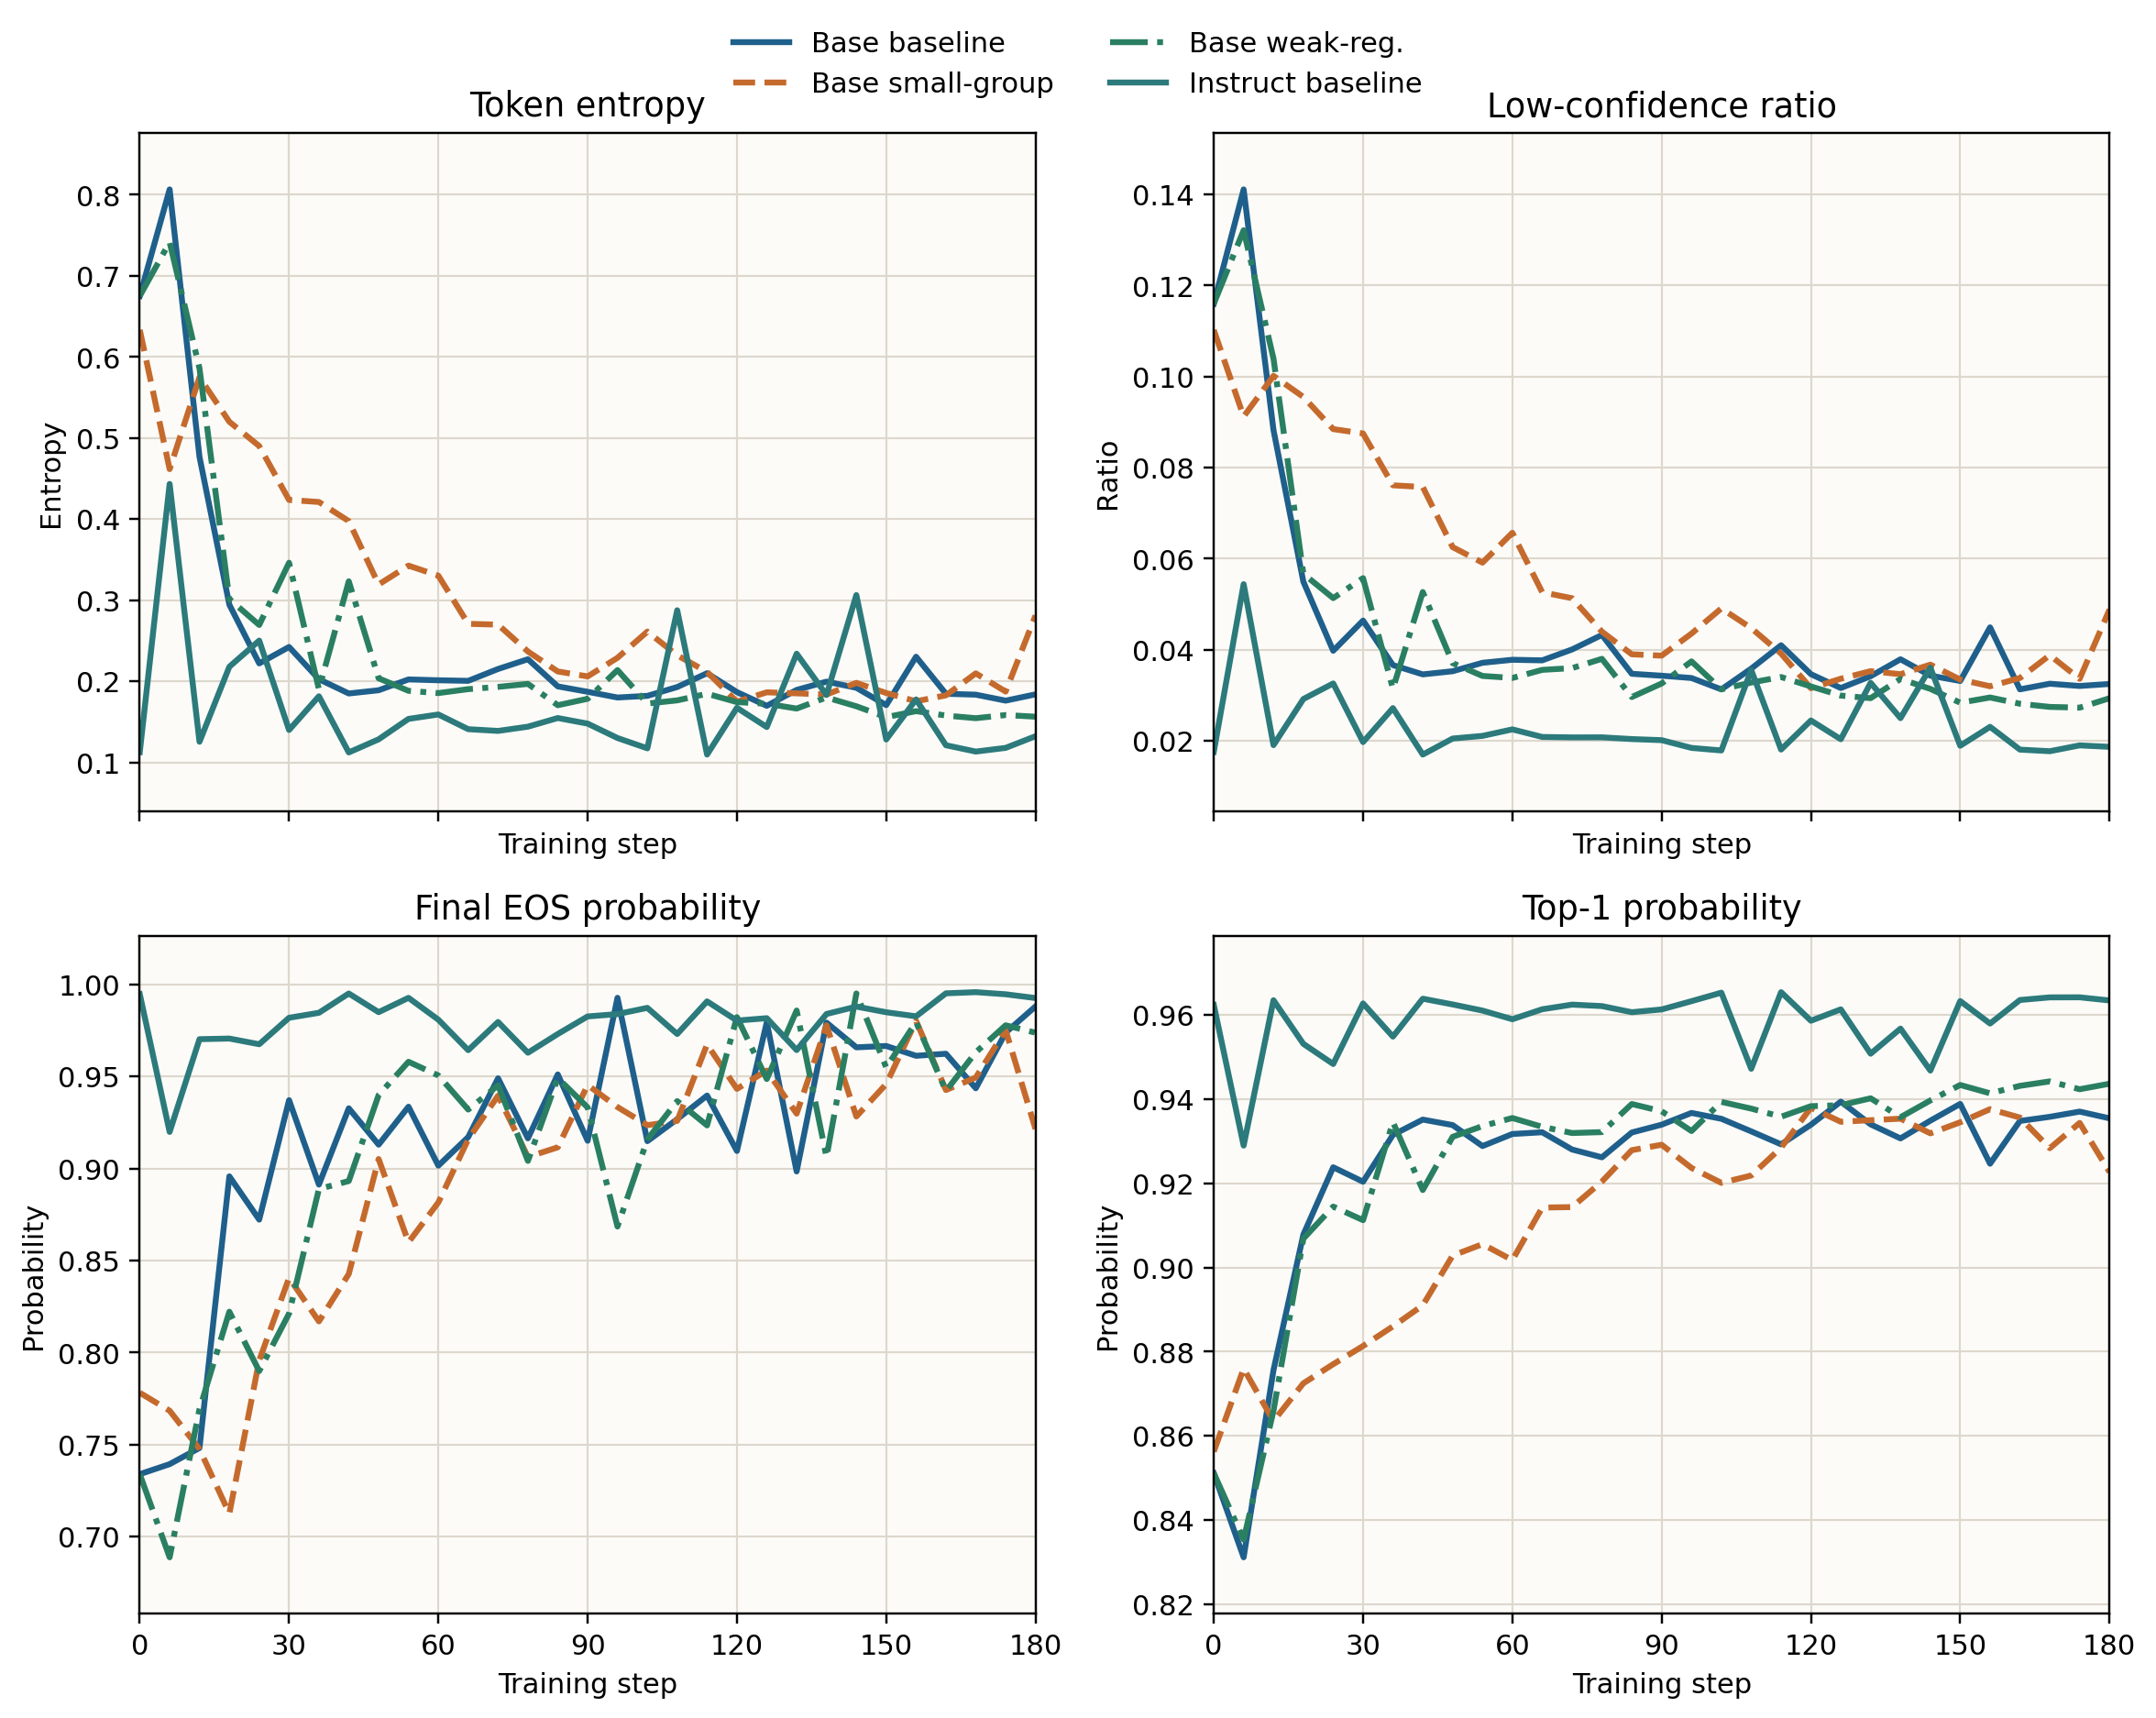
\includegraphics[width=\textwidth,height=0.78\textheight,keepaspectratio]{behavior-detail-main-settings-panel.png}
    \caption{Supplementary comparison among the four non-collapse settings on token entropy, low-confidence ratio, final EOS probability, and top-1 probability.}
    \label{fig:en-appendix-main-settings-panel}
\end{figure}

This comparison reinforces a narrow but important point. The three successful Base settings do not converge to an identical endpoint distribution even when their final scores are close. The weak-regularization setting is the sharpest among them, \texttt{Base n=8} is slightly more moderate, and \texttt{Base n=1} remains visibly looser on entropy and low-confidence mass. The Instruct setting occupies the sharpest region overall, which is consistent with the paper's main interpretation that it begins from a stronger prior and therefore has less behavioral slack to correct.

\clearpage
\section{Correctness-Conditioned Entropy on the Traced Subset}

One natural question is whether the token-level evidence only says that different settings behave differently, or whether correct and wrong responses also separate within a single setting. Figure~\ref{fig:en-appendix-correct-wrong-entropy} gives a small but concrete answer for the traced subset available in \texttt{Base n=1}. It plots final-step token entropy by correctness over eight traced MATH500 questions. The figure is intentionally placed in the appendix because the sample is too small to carry a main claim on its own, yet it is still useful as a directionally consistent piece of evidence.

\begin{figure}[H]
    \centering
    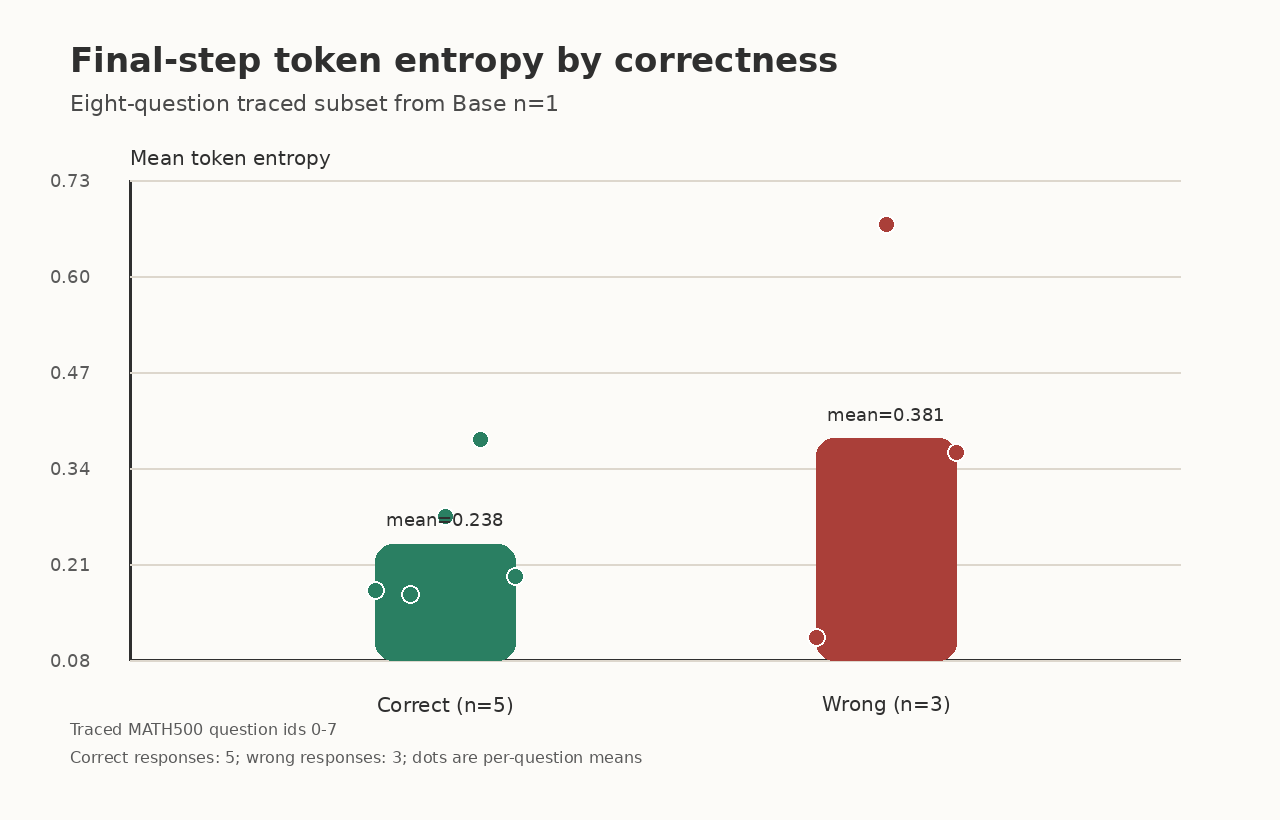
\includegraphics[width=\textwidth,height=0.68\textheight,keepaspectratio]{correct-vs-wrong-entropy.png}
    \caption{Final-step token entropy by correctness on the traced eight-question subset from \texttt{Base n=1}.}
    \label{fig:en-appendix-correct-wrong-entropy}
\end{figure}

Within this traced subset, correct responses end with lower mean token entropy than wrong responses. That is exactly the ordering predicted by the calibration account, but the appendix keeps the evidential weight proportional to the sample size: the figure is best read as supportive micro-evidence rather than as a substitute for the aggregate metrics in the main body.

\section{Interpretation Boundaries for the Appendix Evidence}

The appendix also clarifies two scope boundaries that matter when reading the supplementary material. First, the reward-corruption condition should be interpreted as an extreme wrong-signal control rather than a clean no-signal baseline. Its value is therefore causal rather than symmetric: it shows that meaningful reward integrity matters, but it does not by itself estimate what would happen under a perfectly neutral reward ablation. Second, the legacy full-data references are retained for historical context, not to replace the matched one-shot/full-data comparisons that now anchor the main score-level conclusions.

Those boundaries help explain why the appendix contains both richer comparison material and repeated caveats. The appendix figures and tables are meant to improve readability, not to expand the strength of the core claims beyond what the matched main settings support. In that sense, the appendix is best understood as interpretive scaffolding: it makes the score, calibration, group-size, and reward-integrity story easier to inspect in detail while preserving the same evidential hierarchy as the main text.

\begin{thebibliography}{99}
\bibitem{wang2025oneshotrlvr}
Wang, Y., Yang, Q., Zeng, Z., Ren, L., Liu, L., Peng, B., Cheng, H., He, X., Wang, K., Gao, J., Chen, W., Wang, S., Du, S. S., \& Shen, Y. Reinforcement Learning for Reasoning in Large Language Models with One Training Example. arXiv preprint arXiv:2504.20571, 2025.

\bibitem{deepscaler2025}
Luo, M., Tan, S., Wong, J., Shi, X., Tang, W. Y., Roongta, M., Cai, C., Luo, J., Li, L. E., Popa, R. A., \& Stoica, I. DeepScaleR: Surpassing O1-Preview with a 1.5B Model by Scaling RL. Notion Blog, 2025.

\bibitem{deepseekr1}
DeepSeek-AI et al. DeepSeek-R1: Incentivizing Reasoning Capability in LLMs via Reinforcement Learning. arXiv preprint arXiv:2501.12948, 2025.

\bibitem{kimi15}
Kimi Team et al. Kimi k1.5: Scaling Reinforcement Learning with LLMs. arXiv preprint arXiv:2501.12599, 2025.

\bibitem{ppo}
Schulman, J., Wolski, F., Dhariwal, P., Radford, A., \& Klimov, O. Proximal Policy Optimization Algorithms. arXiv preprint arXiv:1707.06347, 2017.

\bibitem{deepseekmath}
Shao, Z. et al. DeepSeekMath: Pushing the Limits of Mathematical Reasoning in Open Language Models. arXiv preprint arXiv:2402.03300, 2024.

\bibitem{math}
Hendrycks, D. et al. Measuring Mathematical Problem Solving With the MATH Dataset. In Advances in Neural Information Processing Systems (NeurIPS), 2021; arXiv preprint arXiv:2103.03874.

\bibitem{qwen}
Yang, A. et al. Qwen2.5-Math Technical Report: Toward Mathematical Expert Model via Self-Improvement. arXiv preprint arXiv:2409.12122, 2024.

\bibitem{openmathinstruct1}
Toshniwal, S., Moshkov, I., Narenthiran, S., Gitman, D., Jia, F., \& Gitman, I. OpenMathInstruct-1: A 1.8 Million Math Instruction Tuning Dataset. In Advances in Neural Information Processing Systems (NeurIPS), 2024; arXiv preprint arXiv:2402.10176.

\bibitem{openmathinstruct2}
Toshniwal, S., Du, W., Moshkov, I., Kisacanin, B., Ayrapetyan, A., \& Gitman, I. OpenMathInstruct-2: Accelerating AI for Math with Massive Open-Source Instruction Data. arXiv preprint arXiv:2410.01560, 2024.

\bibitem{mammoth2}
Yue, X., Zheng, T., Zhang, G., \& Chen, W. MAmmoTH2: Scaling Instructions from the Web. arXiv preprint arXiv:2405.03548, 2024.

\bibitem{omnimath}
Gao, B. et al. Omni-MATH: A Universal Olympiad Level Mathematic Benchmark For Large Language Models. arXiv preprint arXiv:2410.07985, 2024.

\bibitem{processbench2024}
Zheng, C., Zhang, Z., Zhang, B., Lin, R., Lu, K., Yu, B., Liu, D., Zhou, J., \& Lin, J. ProcessBench: Identifying Process Errors in Mathematical Reasoning. arXiv preprint arXiv:2412.06559, 2024.

\bibitem{automatedprocess2024}
Luo, L., Liu, Y., Liu, R., Phatale, S., Guo, M., Lara, H., Li, Y., Shu, L., Zhu, Y., Meng, L., Sun, J., \& Rastogi, A. Improve Mathematical Reasoning in Language Models by Automated Process Supervision. arXiv preprint arXiv:2406.06592, 2024.

\bibitem{stepdpo2024}
Lai, X., Tian, Z., Chen, Y., Yang, S., Peng, X., \& Jia, J. Step-DPO: Step-wise Preference Optimization for Long-chain Reasoning of LLMs. arXiv preprint arXiv:2406.18629, 2024.

\bibitem{deepseekprover15}
Xin, H. et al. DeepSeek-Prover-V1.5: Harnessing Proof Assistant Feedback for Reinforcement Learning and Monte-Carlo Tree Search. arXiv preprint arXiv:2408.08152, 2024.

\bibitem{rstar2024}
Qi, Z., Ma, M., Xu, J., Zhang, L. L., Yang, F., \& Yang, M. Mutual Reasoning Makes Smaller LLMs Stronger Problem-Solvers. arXiv preprint arXiv:2408.06195, 2024.

\bibitem{testtimecompute2024}
Snell, C., Lee, J., Xu, K., \& Kumar, A. Scaling LLM Test-Time Compute Optimally can be More Effective than Scaling Model Parameters. arXiv preprint arXiv:2408.03314, 2024.

\bibitem{oreo2024}
Wang, H., Hao, S., Dong, H., Zhang, S., Bao, Y., Yang, Z., \& Wu, Y. Offline Reinforcement Learning for LLM Multi-Step Reasoning. arXiv preprint arXiv:2412.16145, 2024.

\bibitem{s1scaling2025}
Muennighoff, N., Yang, Z., Shi, W., Li, X. L., Fei-Fei, L., Hajishirzi, H., Zettlemoyer, L., Liang, P., Cand{\`e}s, E., \& Hashimoto, T. s1: Simple test-time scaling. arXiv preprint arXiv:2501.19393, 2025.

\bibitem{limo2025}
Ye, Y., Huang, Z., Xiao, Y., Chern, E., Xia, S., \& Liu, P. LIMO: Less is More for Reasoning. arXiv preprint arXiv:2502.03387, 2025.

\bibitem{limr2025}
Li, X., Zou, H., \& Liu, P. LIMR: Less is More for RL Scaling. arXiv preprint arXiv:2502.11886, 2025.
\end{thebibliography}

\end{document}
